\begin{filecontents*}{data.csv}
    in gdp
    1991  2768900924
    1992  1761774062
    1993  1717739533
    1994  1737565752
    1995  1760478791
    1996  1789413624
    1997  1842918632
    1998  1894645346
    2000  1732502852
\end{filecontents*}

\lohead{Hörmann Stefan}
\chapter{Mechanik}
\section{Einleitung}

\section{Anforderung}
\label{sec:Anforderung}
Die Arbeit des mechanischen Teiles besteht darin, eine Maschine,
die Spielkarten mischen und ausgeben kann, zu entwerfen, zu konstruieren
und einen Teilaufbau durchzuführen. Die Maschine sollte in der Lage
sein, 20 Spielkarten zu mischen und diese nach einem Spielmodus, der
zuvor am LCD gewählt wurde, auszugeben. Das Ziel ist es, die Spielkarten
optimal zu mischen, aber die Maschine dennoch kompakt und optisch
ansprechend zu entwerfen. Weiters sollte der Mischvorgang und die
Ausgabe der Karten nicht zu lange dauern. Die Teile der Maschine
sollten so konstruiert werden, dass sie kostengünstig produziert
werden können. Zum Schluss sollte noch ein Teilaufbau der Maschine
geschehen, um die Funktionalität der einzelnen Bereiche zu testen
und gegebenenfalls zu verbessern.

\section{Problemstellungen}
Ein Problem ist das begrenzte Budget unseres Teams, somit sind
wir auf gewisse Produktionsarten unserer Bauteile beschränkt.
Die Oberfläche der Karten ist ein
weiteres Problem, da diese sich nicht immer separieren lassen. Dies
hat zur Folge, dass oft zwei oder mehrere Karten auf einmal genommen
werden und das Konzept des optimalen Mischens zerstört.

\newpage
\subsection{Zeitplan}

\begin{figure}[H]
    \centering
    \scalebox{0.6}{
    \begin{ganttchart}[
    hgrid style/.style={black, dotted},
    calendar week text={\currentweek},
    vgrid={*6{white},*1{black,dotted}},
    x unit=1mm,
    group label font= \Large,
    y unit chart=9mm,
    y unit title=12mm,
    time slot format=isodate,
    time slot unit=year
    link/.style={->, thick}
    ]{2019-09-2}{2020-03-15}
        \gantttitlecalendar{year, month=name, week}\\

        \ganttgroup[group/.append style={draw=none}]
        {Variantenvergleich}{2019-09-02}{2019-11-13}\\ [grid]
        \ganttbar[]{Variantenvergleich des Gesamtsystems}{2019-09-02}{2019-10-15}\\ [grid]
        \ganttbar[]{Variantenvergleich der Einzelbauteile}{2019-10-03}{2019-11-8}\\ [grid]
        \ganttbar[]{Variantenfreeze des Gesamtsystems}{2019-11-2}{2019-11-13}\\ [grid]
        \ganttnewline[thick, black]

        \ganttgroup[group/.append style={draw=none}]{Konstruktion}{2019-10-28}{2020-01-20}\\ [grid]
        \ganttbar[]{Konstruktion des Lagerradmoduls}{2019-10-28}{2019-11-30}\\ [grid]
        \ganttbar[]{Konstruktion des Kartenhalterungsmoduls}{2019-11-28}{2019-12-27}\\ [grid]
        \ganttbar[]{Konstruktion der Kartenentnahme}{2019-12-27}{2020-01-03}\\ [grid]
        \ganttbar[]{Fertigstellung des Gesamtsystems}{2020-01-03}{2020-01-20}\\ [grid]
        \ganttnewline[thick, black]

        \ganttgroup[group/.append style={draw=none}]{Fertigung}{2019-12-15}{2020-02-21}\\ [grid]
        \ganttbar[]{Fertigung der 3D-Druck Teile}{2019-12-15}{2020-01-31}\\ [grid]
        \ganttbar[]{Fertigung der Frästeile}{2019-12-28}{2020-01-08}\\ [grid]
        \ganttbar[]{Fertigung des Gehäuses}{2020-01-20}{2020-02-21}\\ [grid]


        \ganttnewline[thick, black]

        \ganttgroup[]{Dokumentation}{2019-12-07}{2020-02-28}\\ [grid]

    \end{ganttchart}
    }
    \caption{Zeitplan Bereich Mechanik}
\end{figure}

\section{Konzepte}

\subsection{Anforderungen}

\begin{enumerate}
    \item \textbf{Kosten}  \\
    Der Automat sollte möglichst kostengünstig produziert werden,
    da das vorhandene Budget gering ist. Dies hat zur Folge, dass keine teuren Motoren
    oder kostenspieligen Bauteile zum Einsatz kommen können.
    \item \textbf{Schnelligkeit} \\
    Um ein gutes Spielerlebnis zu garantieren, sollte der Automat keine
    lange Mischzeit aufweisen. Das Zeitfenster, in welchem man die Karten einführt und den
    Mischen-Button betätigt, bis hin zur Ausgabe der ersten Karte, sollte möglichst gering sein.
    \item \textbf{Mischgenauigkeit} \\
    Die Mischgenauigkeit ist die am schwersten gewichtete Anforderung,
    da es das Ziel ist, ein optimales Mischen der Spielkarten zu erreichen.
    Diese Anforderung mit größter Priorität erfüllt werden.
    \item \textbf{Optik und Größe} \\
    Die Optik des Automaten soll schlicht gehalten werden. Der Automat sollte ein ansprechendes Design aufweisen und
    auf Messen und andere Ausstellungen präsentierbar sein. Die Maschine
    sollte jedoch auch stabil konstruiert werden, muss aber dennoch mobil bleiben und
    darf eine gewisse Größe nicht überschreiten.
\end{enumerate}

\subsection{Variantenvergleich}
Um alle oben angegebenen Anforderungen zu erfüllen, wurden mehrere Konzepte entworfen und diese verglichen.

\subsubsection{Variante 1 - Linearachsen}


\begin{figure}[hb]
    \centering
    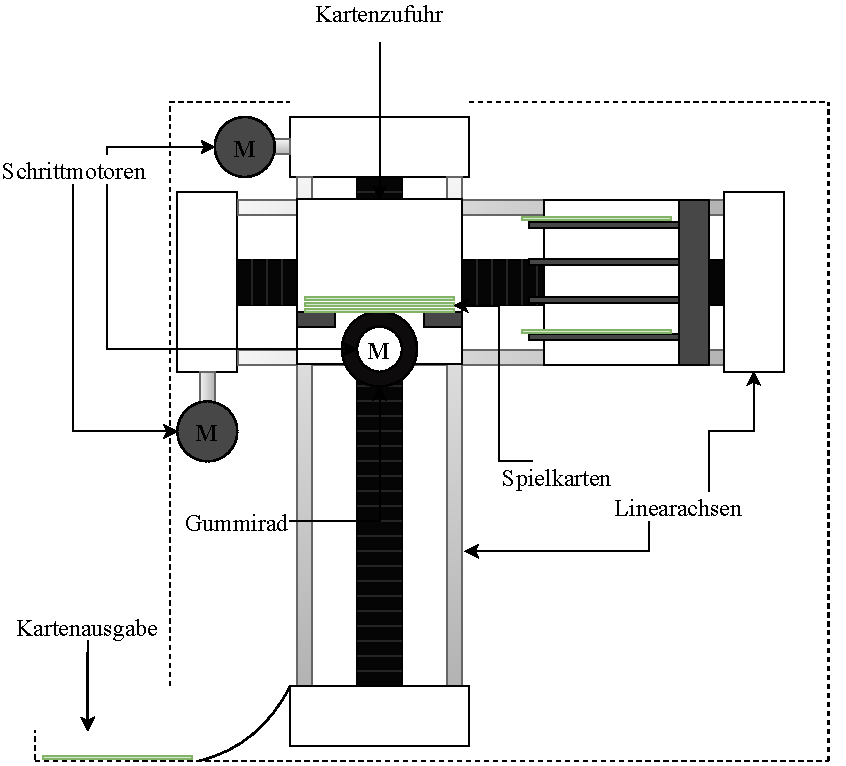
\includegraphics[scale=0.9,page=1]{fig/mech/Version1}
    \caption{Variante 1}

\end{figure}


Das erste Konzept würde mit zwei Linearachsen realisiert werden, diese wären im rechten Winkel zueinander
angeordnet. Die senkrechte Linearachse ist mit einer Halterung versehen, welche in der Lage ist,
ein Kartendeck aufzunehmen und die unterste Karte mithilfe eines Ausgaberades weiterzubefördern. Die zweite
Linearachse besitzt 4 Fächer, in welcher die Karten von der ersten Linearachsenausgabe befördert werden.
Dies wird realisiert, indem die erste Linearachse zyklisch zufällige Fächer anfährt. Befinden sich alle Karten im Lager, so fährt die erste Linearachse nach unten, danach
fährt die zweite Linearachse impulsiv nach links und bremst schlagartig ab, um die Karten aus dem Lager zu werfen. Diese fallen
senkrecht in das Lager der ersten Linearachse, wo sie nun zum Ausgeben durch das Ausgaberad bereitliegen. \\



Durch die schnelle Bewegung der Linearachsen ist es möglich, einen schnellen Mischprozess zu erreichen,
auch die Tatsache, dass es nur ein rotierendes Rad sowie zwei bewegliche Linearachsen gibt, führt dazu, dass
Fehler bei Bewegungen nur selten auftreten. Jedoch besteht durch den hohen Aufbau der Maschine und durch die hohe
Position der zweiten Linearachse, die sich horizontal bewegt, die Gefahr des Umkippens der Maschine. Somit wäre
keine Stabilität mehr gegeben. Der Preis der Linearachsen ist ein weiterer Nachteil dieses Konzepts. Eine Linearachse,
die unseren Anforderungen entspricht, wäre mit Motor und Schlitten zu teuer für unser Budget. \\

\textbf{Vorteile:}
\begin{itemize}
    \item Schnelles Mischen
    \item Wenige Fehlerquellen
\end{itemize}
\textbf{Nachteile:}
\begin{itemize}
    \item Teuer
    \item Großer Aufbau %Genaueres Beschreiben der Vor und Nachteile?
    \item Instabil
\end{itemize}

\subsubsection{Variante 2 - Lagerrad mit Ausgaberäder}

\begin{figure}[H]
    \centering
    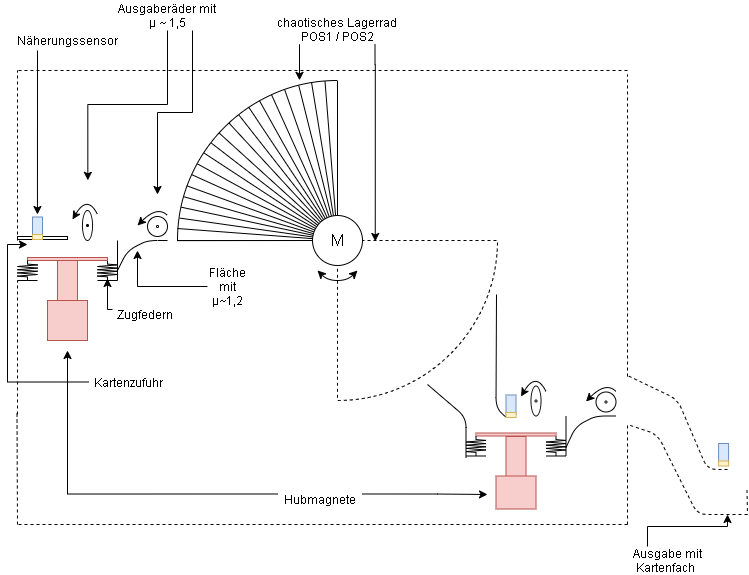
\includegraphics[scale=0.6,page=1]{fig/mech/V1904-Page-2.png}
    \caption{Variante 2}
\end{figure}

Beim zweiten Konzept wird als Lager ein Viertel eines Zylinders benutzt. In diesem befinden
sich verschiedene Fächer, in der die Karten eingelagert werden. Dieser wird mit einem Motor betrieben
und dreht sich somit in die vorgegebenen Positionen, um das Einlagern und das Ausgeben der Karten zu ermöglichen.
Die Karteneingabe erfolgt über eine Öffnung in der Topplatte der Maschine. Dort befindet sich ein Hubmagnet, der die Karten
zum Weiterbefördern nach oben drückt. Ein kapazitiver Sensor sorgt dafür, dass sichergestellt werden kann, dass sich Karten auf dem Hubmagnet befinden.
Um eine Karte in das Lager zu befördern, wird der Hubmagnet eingeschaltet und drückt das Kartendeck auf das erste Ausgaberad. Um die Kraft des Hubmagnetes zu minimieren, sind Zugfedern angebracht.
Das Ausgaberad befördert eine Karte weiter zum zweiten Ausgaberad, welches widerum sicherstellt, dass nur eine Karte in das Lagerrad transportiert wird.
Danach dreht das Lagerrad auf eine andere, zufällig ausgewählte Position.
Dieser Prozess wird so lange wiederholt, bis alle Karten im Lagerrad befinden.
Infolgedessen dreht sich dieses, mit einer hohen Geschwindigkeit und wirft somit die Karten in eine Auffangführung.
Diese Auffangführung befördert die Karten in einen gleichen Mechanismus wie bei der Vorderseite der Maschine, in dem sie von einem Hubmagneten nach oben gedrückt werden und von zwei Ausgaberädern zur
Kartenentnahme geschoben werden.
Da die Karten zum Schluss nach einem Spielmodus und somit in einer bestimmten Anzahl ausgegeben werden, befindet sich ein kapazitiver Sensor auch bei der Ausgabe der Karten,
welcher überprüfen soll, ob die Karten von dem Spieler bereits genommen wurden oder nicht.\\

Durch den niedrigen Aufbau, der durch ein "fließbandartiges" Befördern der Karten erreicht wird, besitzt die Maschine ein hohes Maß an Stabilität. Jedoch entsteht dadurch auch der Nachteil, dass die Maschine sehr lang wird. Da dieses
Konzept fünf bewegliche Räder besitzt sowie zwei Hubmagneten, ist es anfällig für Fehler beim Bewegungsablauf.
Außerdem kann nicht garantiert werden, dass nur eine Karte in das Lagerrad befördert wird. Dies würde das Konzept des optimalen
Mischens negieren. Die vielen Bauteile führen auch zu teureren Anschaffungskosten, welche möglichst niedrig gehalten werden sollen.\\

\textbf{Vorteile:}
\begin{itemize}
    \item Stabil
    \item Niedriger Aufbau
\end{itemize}
\textbf{Nachteile:}
\begin{itemize}
    \item Langes Gehäuse
    \item Viele bewegliche Bauteile / Fehlerquellen
\end{itemize}

\subsubsection{Variante 3 - Lagerrad mit Saugnäpfe}

\begin{figure}[H]
    \centering
    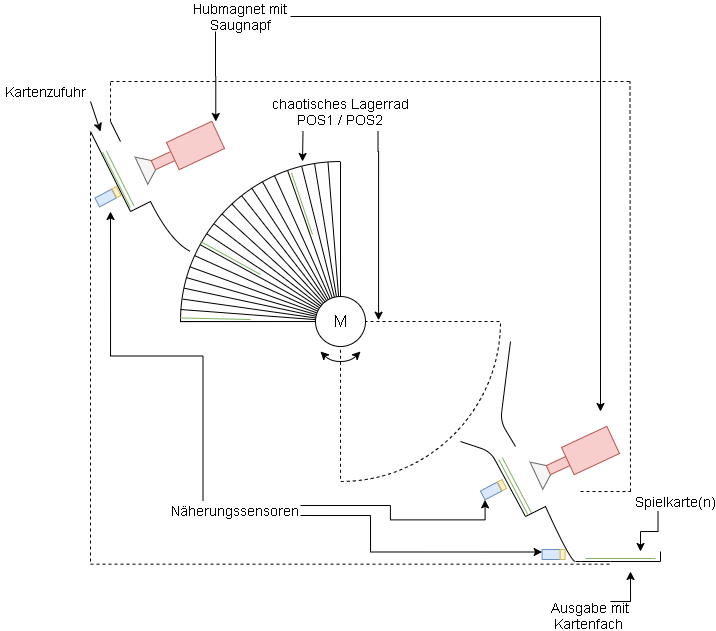
\includegraphics[scale=0.6,page=1]{fig/mech/AufbauReshuffledV3}
    \caption{Variante 3}
\end{figure}

Das dritte Konzept besitzt ein identes Lagersystem wie das Zweite: ein Lagerrad, welches in Fächer unterteilt ist und über einen Motor diverse Positionen einnehmen kann.
Das Kartendeck wird auf der Oberseite der Maschine eingeführt. Dort liegt es schräg in einem Winkel von ca. 60°. Um sicherzustellen, dass sich Karten in dieser Halterung befinden,
ist ein kapazitiver Sensor an der Unterseite angebracht.
Ein Hubmagnet, der orthogonal zu den Karten über der Halterung angebracht ist, saugt jede Karte einzeln an indem ein Saugnapf, der an einem Hubmagneten
befestigt ist, heruntergedrückt wird. Ist die Karte angesaugt, so wird der Hubmagnet von einer Feder in seine Ausgangsstellung zurückgebracht.
Dabei wird die Spielkarte durch eine Platte abgestreift und fliegt somit in ein Fach des
Lagerrades hinein. Dieser Prozess wird so lange wiederholt, bis sich alle Spielkarten des Kartendecks im Lagerrad befinden.
Sind alle Karten im Lagerrad, so dreht sich dieses und wirft die Karten auf der Rückseite der Maschine in eine Führung, welche die Karten in eine zweite Halterung befördert.
Diese zweite Halterung ist ident aufgebaut wie die erste.
Die Karten werden nun wieder einzeln vom Saugnapf angesaugt und in ein Ausgabefach am Ende der Maschine befördert. Im Ausgabefach befindet sich
ein kapazitiver Sensor. Dieser überprüft, ob die Karten vom Spieler bereits genommen wurden.\\

Durch die wenigen Bauteile, die dieses Konzept besitzt, ist das Konzept wenig fehleranfällig bei Bewegungsabläufen.
Außerdem ist es durch die wenigen Bauteile im Vergleich billiger als die anderen Konzepte.
Ein Problem dieses Konzepts ist seine Höhe und, dass das Lagerrad sich in der Mitte der Maschine befindet.
Jedoch ist durch das geringe Gewicht des Lagerrades noch immer genügend Stabilität vorhanden, auch wenn sich dieses mit voller Geschwindigkeit dreht. \\

\textbf{Vorteile:}
\begin{itemize}
    \item Billig
    \item Wenig bewegliche Bauteile
\end{itemize}
\textbf{Nachteile:}
\begin{itemize}
    \item Hoher Aufbau
\end{itemize}

\subsection{Ausgaberäder}
Um die Karten weiterzubefördern, werden bei zwei Konzepten Ausgaberäder benutzt, für diese gibt es verschiedene Konzepte, die sich in Preis, Herstellung und Funktionalität unterscheiden.\\
Das Ausgaberad ist mit einem Motor verbunden, welcher dafür sorgt, dass eine Karte von dem Kartendeck weiterbefördert wird.
\begin{itemize}
    \item \textbf{Rundes Ausgaberad}
\end{itemize}

\begin{figure}[H]
    \centering
    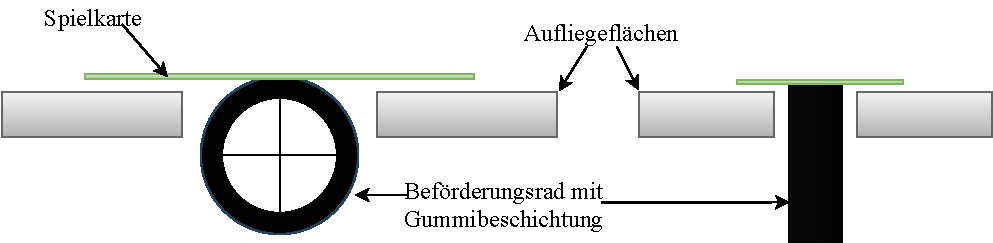
\includegraphics[scale=0.9,page=1]{fig/mech/RundesAusgaberad-Page-1}
    \caption{Rundes Ausgaberad}
\end{figure}

Die einfachste Möglichkeit dieses Rad zu entwerfen, wäre ein einfaches rundes Ausgaberad.
Dieses Rad wäre mit einer Schicht umhüllt, welche die Reibung zwischen dem Rad und der Karte erhöht.
Das runde Rad wäre einfach zu fertigen und würde somit wenig Kosten verursachen und nur einen geringen Zeitaufwand haben.
Jedoch ist das Rad in der Lage, mehr als nur eine Karte mit sich zu ziehen, da es durchgehen Kontakt mit der Spielkartenoberfläche hat.
Dies hätte zur Folge, das mehrere Spielkarten zugleich weiterbefördert werden.
\begin{itemize}
    \item \textbf{Elliptisches Ausgaberad}
\end{itemize}

\begin{figure}[H]
    \centering
    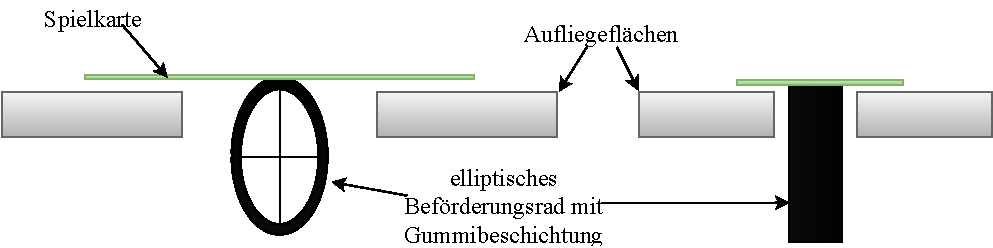
\includegraphics[scale=0.9,page=1]{fig/mech/ElliptischesAusgaberad}
    \caption{Elliptisches Ausgaberad}
\end{figure}


Ein elliptisches Ausgaberad wäre das nächste Konzept.
Dieses Rad wird auch wie beim ersten Konzept mit einem Motor verbunden, um somit Karten zu befördern.
Durch die elliptische Form des Rades herrscht kein durchgehender Kontakt mit der Oberfläche der Spielkarte, aus diesem Grund ist die Chance, das mehrere
Karten zugleich befördert werden, minimiert.
Jedoch setzt dies auch einen Motor voraus der in kurzer Zeit ein hohes Drehmoment entwickelt, da die
Karten schlagartig befördert werden.
Das elliptische Rad würde in der Produktion auch mehr Kosten verursachen und wäre zeitintensiver in der Herstellung. \\

\begin{itemize}
    \item \textbf{Vergleich der Ausgaberäder}
\end{itemize}

Da das primäre Ziel unserer Arbeit das perfekte Mischen der Spielkarten ist, wäre es besser, das elliptische Ausgaberad in Betracht zu ziehen.
Die Kosten, die durch die aufwendigere Herstellung entstehen wären überschaulich und somit wäre es von Vorteil, dieses Konzept zu wählen.
Durch die Tatsache, dass das elliptische Rad das Kartendeck nur jede halbe Umdrehung berührt und nicht dauerhaft, muss ein Motor für die Räder eingesetzt werden, der sich schnell genug dreht, um eine Karte mit einer Berührung
des Rades "herauszuschießen".
Dies würde aber keine zusätzlichen Kosten verursachen.
Aus diesen Gründen fällt die Wahl auf das elliptisches Ausgaberad. \\

\subsection{Klemmmechanismen}
Um beim Ausgeben und beim Weiterbefördern der Karten die Chance zu minimieren, dass mehrere Karten auf einmal weiterbefördert werden, wird ein
Klemmmechanismus benutzt.
Dieser sorgt dafür, dass die Karten von außen geklemmt werden und somit nur die unterste Karte durch das Drehen des
Ausgaberades weiterbefördert wird.

\begin{itemize}
    \item \textbf{Primitiver Klemmmechanismus}
\end{itemize}

\begin{figure}[H]
    \centering
    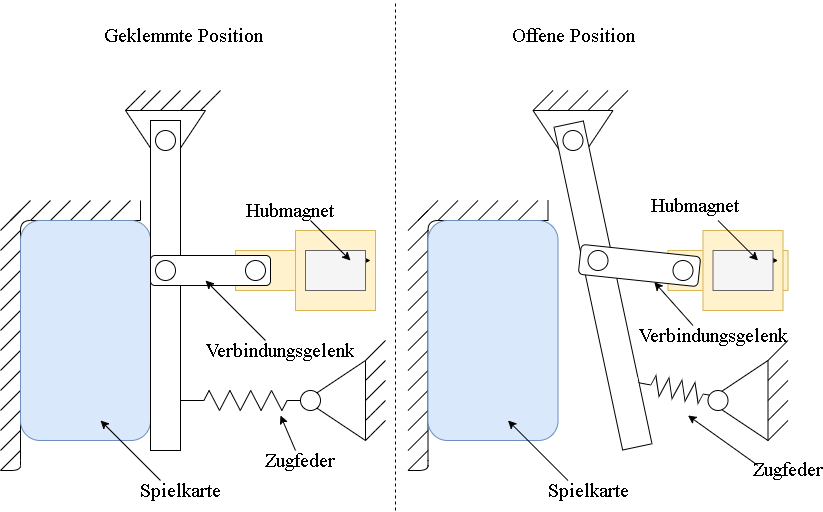
\includegraphics[scale=0.5,page=1]{fig/mech/Klemmmechanissmus-Page-1.png}
    \caption{Primitiver Klemmmechanismus}
\end{figure}

Dieser Klemmmechanismus ist der primitivste und einfachste, dadurch aber auch der billigste.
Die Karten werden auf der einen Seite an eine feste Wand gedrückt, auf der anderen Seite werden sie durch ein bewegliches Gelenk fixiert.
Dieses Gelenk wird durch das Einschalten des Hubmagneten in die geschlossene Position bewegt.
Soll das Gelenk wieder öffnen, so wird der Hubmagnet ausgeschaltet und eine Zugfeder zieht das Gelenk wieder in seine Ausgangsposition zurück.

\begin{itemize}
    \item \textbf{Komplexer Klemmmechanismus}
\end{itemize}

\begin{figure}[H]
    \centering
    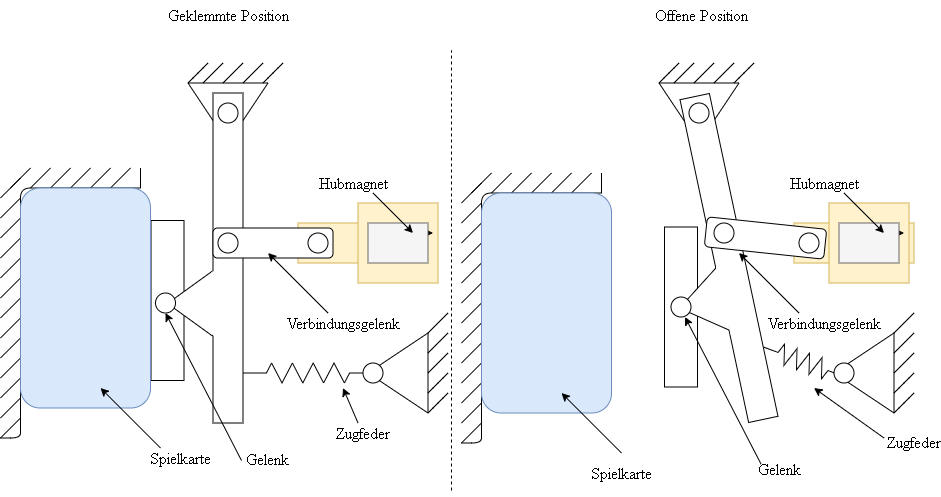
\includegraphics[scale=0.5,page=1]{fig/mech/Klemmmechanissmus-Page-2.png}
    \caption{Komplexer Klemmmechanismus}
\end{figure}

Bei diesem Mechanismus werden die Karten auf der einen Seite durch eine feste Wand geklemmt, auf der anderen werden sie durch ein Gelenk geklemmt.
Dieses Gelenk ist beweglich und gleicht somit verschiedene Kartengrößen aus.
Um das Gelenk dieses Konzeptes zu schließen, wird ein Hubmagnet benötigt.
Wird dieser eingeschaltet, so schließt das Gelenk und passt sich der Kartengröße an.
Soll es wieder geöffnet werden, so wird der Hubmagnet ausgeschaltet und eine Zugfeder bringt den Mechanismus wieder in den Grundzustand.
Dieses Konzept ist aufwendiger zu realisieren wie das erste, jedoch ist es möglich verschiedene Kartengrößen zu klemmen.

\begin{itemize}
    \item \textbf{Gummi Klemmmechanismus}
\end{itemize}

\begin{figure}[H]
    \centering
    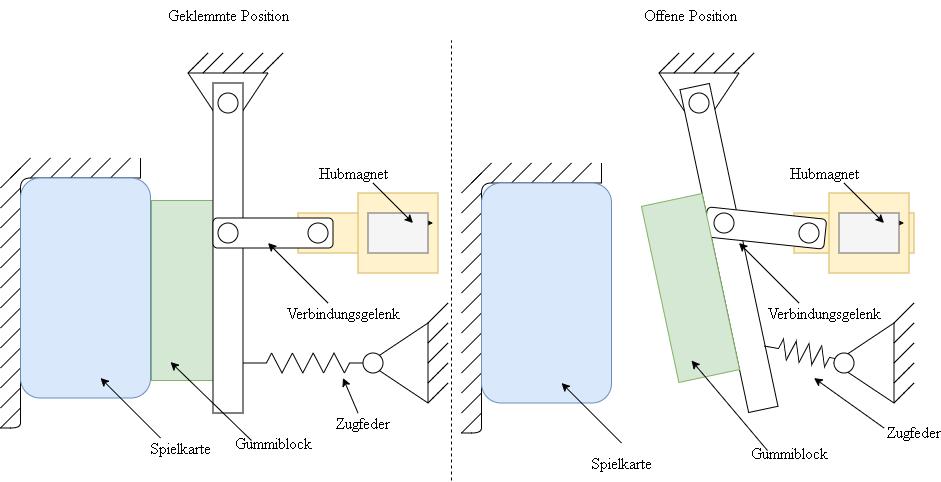
\includegraphics[scale=0.5,page=1]{fig/mech/Klemmmechanissmus-Page-3.png}
    \caption{Gummi Klemmmechanismus}
\end{figure}

Der letzte Mechanismus ist funktionsmäßig gleich wie der primitive Klemmmechanismus, der einzige Unterschied besteht aus dem
gummiartigen Block, der sich auf der Klemmfläche befindet.
Dieser soll sich den Karten anpassen und sorgt dafür, dass alle Karten gleichmäßig geklemmt werden.
Außerdem erhöht es die Reibung zwischen den Karten und der Klemmoberfläche.
Dieses Konzept wäre in der Herstellung vergleichsweise einfach zu realisieren und dadurch auch billig.


\begin{itemize}
    \item \textbf{Vergleich der Klemmmechanismen}
\end{itemize}

Da alle Mechanismen die gleiche Anzahl an Bauteile erfordern, spielt der Preis bei dieser Auswahl keine große Rolle.
Aus diesem Grund sind die Kriterien Funktionalität und Aufwand in der Produktion.
Der erst Mechanismus wäre der einfachste in der Produktion, jedoch hat er durch sein nicht anpassungsfähiges Klemmgelenk Probleme mit verschiedenen Kartengrößen.
Aus diesem Grund wird dieses Konzept ausgeschlossen.
Der zweite Mechanismus wäre der komplexe Klemmmechanismus, welcher sich zwar verschiedenen Kartengrößen anpassen würde, aber etwas aufwendiger in der
Produktion wäre und somit auch nicht die bevorzugte Wahl zu sein vermag.
Da er einfach in der Produktion ist und sich verschiedenen Kartengrößen anpassen kann, fällt die Wahl jedoch auf den Gummiklemmmechanismus.

\subsection{Seperation der Karten}
Da bei Variante 3 Saugnäpfe mit Unterdruckprinzip in Verwendung kommen würden, liegt das Problem vor,
dass die Karten aneinander haften. Dieses Problem entsteht durch den Unterdruck, der beim Aufpressen des Saugnapfes entsteht.
Um zu garantieren, dass nur eine Karte in das Lager befördert oder ausgegeben wird, müssen diese aneinander haftenden Karten getrennt werden.

\begin{enumerate}
    \item \textbf{Selbständiges Loslösen der Karten}\\
    Die billigste und primitivste Möglichkeit die Karten zu separieren wäre abzuwarten, bis Luft zwischen den Karten von außen eindringt und alle Karten sich durch die Schwerkraft
    von der eigentlich angesaugten Karte getrennt haben.
    Jedoch zeigten Versuche, welche durchgeführt wurden, dass dies zu lange dauern und das Spielerlebnis somit beeinflussen würde.

    % Please add the following required packages to your document preamble:
    % \usepackage{multirow}
    \begin{table}[H]
        \centering
        \scalebox{0.9}{
        \begin{tabular}{|c|c|c|c|c|c|c|c|}
            \hline
            \textbf{}                         & \multicolumn{7}{c|}{\textbf{Sekunden}}                                                                  \\ \hline
            \multirow{21}{*}{\textbf{Karten}} &    & 1. Durchgang & 2. Durchgang & 3. Durchgang & 4. Durchgang & 5. Durchgang        & Mittelwert       \\ \cline{2-8}
            & 20 & 9.69         & 9.32         & 8.92         & 8.54         & 4.53                & 8.2              \\ \cline{2-8}
            & 19 & 9.1          & 9.97         & 13.82        & 6.71         & 7.75                & 9.47             \\ \cline{2-8}
            & 18 & 15.39        & 8.93         & 6.51         & 13.05        & 15.25               & 11.826           \\ \cline{2-8}
            & 17 & 6.45         & 6.67         & 6.16         & 8.06         & 6.97                & 6.862            \\ \cline{2-8}
            & 16 & 10.76        & 6.52         & 10.62        & 11.37        & 6.97                & 9.248            \\ \cline{2-8}
            & 15 & 12.81        & 6.45         & 16.22        & 8.74         & 4.7                 & 9.784            \\ \cline{2-8}
            & 14 & 3.46         & 9.78         & 11.72        & 5.85         & 6.39                & 7.44             \\ \cline{2-8}
            & 13 & 4.85         & 8.18         & 10.77        & 10.5         & 3.43                & 7.546            \\ \cline{2-8}
            & 12 & 15.1         & 5.37         & 12.36        & 8.54         & 12.31               & 10.736           \\ \cline{2-8}
            & 11 & 15.83        & 6.32         & 5.58         & 5.08         & 1.12                & 6.786            \\ \cline{2-8}
            & 10 & 7.14         & 8.4          & 11.21        & 12.76        & 4.43                & 8.788            \\ \cline{2-8}
            & 9  & 7.48         & 6.24         & 11.87        & 4.32         & 6.36                & 7.254            \\ \cline{2-8}
            & 8  & 4.68         & 5.65         & 8.61         & 5.2          & 4.41                & 5.71             \\ \cline{2-8}
            & 7  & 9.73         & 8.29         & 9.13         & 5.35         & 11.2                & 8.74             \\ \cline{2-8}
            & 6  & 5.41         & 5.16         & 8.05         & 4.98         & 9.73                & 6.666            \\ \cline{2-8}
            & 5  & 6.06         & 4.81         & 7.8          & 4.73         & 7.19                & 6.118            \\ \cline{2-8}
            & 4  & 4.86         & 9.87         & 7.74         & 9.51         & 7.4                 & 7.876            \\ \cline{2-8}
            & 3  & 4.54         & 11.31        & 4.31         & 6.74         & 10.82               & 7.544            \\ \cline{2-8}
            & 2  & 4.83         & 2.19         & 4.13         & 3.78         & 5.71                & 4.128            \\ \cline{2-8}
            &    &              &              &              &              & \multicolumn{2}{c|}{Mittelwert: 7.932} \\ \hline
        \end{tabular}}
        \caption{Haftzeit der Karten}
        \label{tab:my-table}
    \end{table}

    \begin{figure}[H]
        \centering
    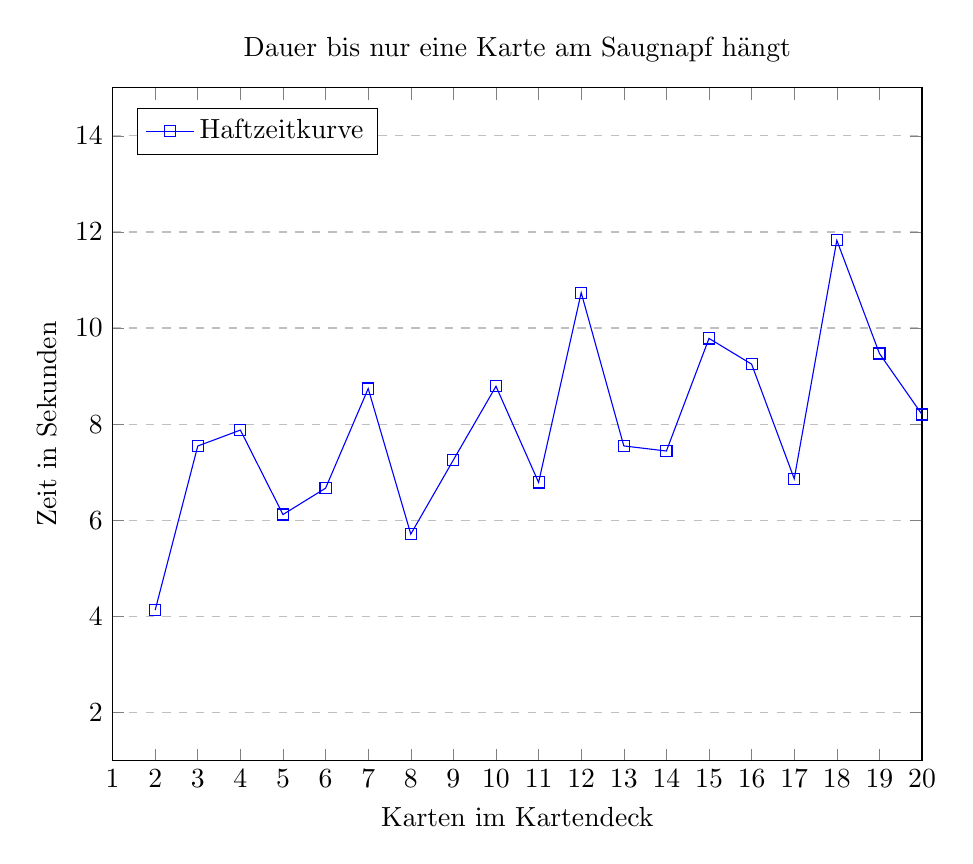
\begin{tikzpicture}
        \begin{axis}[
            scale=1.5,
            title={Dauer bis nur eine Karte am Saugnapf hängt},
            xlabel={Karten im Kartendeck},
            ylabel={Zeit in Sekunden},
            xmin=1, xmax=20,
            ymin=1, ymax=15,
            xtick={1,2,3,4,5,6,7,8,9,10,11,12,13,14,15,16,17,18,19,20},
            ytick={0,2,4,6,8,10,12,14,16,18,20},
            legend pos=north west,
            ymajorgrids=true,
            grid style=dashed,
        ]

            \addplot[
                color=blue,
                mark=square,
            ]
            coordinates {
                (2,4.128)(3,7.544)(4,7.876)(5,6.118)(6,6.666)(7,8.74)(8,5.71)(9,7.254)(10,8.788)(11,6.786)(12,10.736)(13,7.546)(14,7.44)(15,9.784)(16,9.248)(17,6.862)(18,11.826)(19,9.47)(20,8.2)
            };
            \legend{Haftzeitkurve}
        \end{axis}
    \end{tikzpicture}
        \caption{Diagramm Haftzeit der Karten}
        \label{fig:Haftzeit}
    \end{figure}



    Wie man in \autoref{tab:my-table} und in \autoref{fig:Haftzeit} erkennen kann, dauert es im Durchschnitt 7,932 Sekunden bis sich nur mehr die
    eigentlich angesaugte Karte am Saugnapf befindet.
    Der Versuch wurde mit 1kg Ansaugdruck durchgeführt.
    Es gab insgesamt fünf Durchgänge, bei denen alle Möglichkeiten der Kartenanzahlen im Kartendeck berücksichtigt wurden.
    So saugte der Saugnapf bei der ersten Durchgangsreihe die erste Karte an, die auf 19 anderen Karten liegt, bis hin zu einem Saugnapf, der
    eine Karte ansaugt, die nur auf einer einzelnen anderen Karte liegt.

    \textbf{Vorteile:}
    \begin{itemize}
        \item Billig
        \item Keine zusätzlichen Bauteile benötigt
    \end{itemize}
    \textbf{Nachteile:}
    \begin{itemize}
        \item Lange Wartezeit
        \item Unzuverlässig
    \end{itemize}

    \item \textbf{Rütteln}\\\\
    Ein weiteres Konzept, um die angesaugten Karten von den anderen zu trennen, wäre die Karten minimal zu rütteln.
    Da die angesaugte Karte viel stärker an dem Saugnapf haftet als jene Karten, welche an der angesaugten Karte haften,
    könnte der Hubmagnet oder der Ansaugmechanismus leicht gerüttelt werden.
    So würden die anderen Karten schneller den Unterdruck untereinander verlieren und würden sich somit schon in kurzer Zeit separieren lassen.
    Jedoch müsste für dieses Konzept ein Mechanismus entwickelt und produziert werden, der nur einen ausgewählten Bereich rüttelt. Dies wäre mit weiteren Bauteilkosten und
    Aufwand verbunden.

    \textbf{Vorteile:}
    \begin{itemize}
        \item Zuverlässig
    \end{itemize}
    \textbf{Nachteile:}
    \begin{itemize}
        \item Teurer
        \item Zusätzliche Bauteile
        \item Zusätzliche Größe
    \end{itemize}



    \item \textbf{Abstreifbürsten}\\
    Bei diesem Konzept sind bürstenartige Abstreifvorrichtungen in der Kartenhalterung angebracht.
    Diese Bürsten sollen beim Aufheben der
    angesaugten Karte die anderen Karten, die mitgehoben wurden, abstreifen.
    Dabei ist es wichtig, dass die Bürste den richtigen Widerstand aufbringt.
    Ist der Widerstand zu hoch, wird auch die eigentlich angesaugt Karte mit abgestreift.
    Ist er jedoch zu niedrig, ist es möglich, dass die anderen Karten,
    die mitgehoben werden, nicht abgestreift werden.

    \textbf{Vorteile:}
    \begin{itemize}
        \item Zuverlässig
        \item Billig
    \end{itemize}
    \textbf{Nachteile:}
    \begin{itemize}
        \item Karten werden seitlich abgenützt
        \item Komplizierter Einbau
    \end{itemize}

    \begin{figure}[H]
        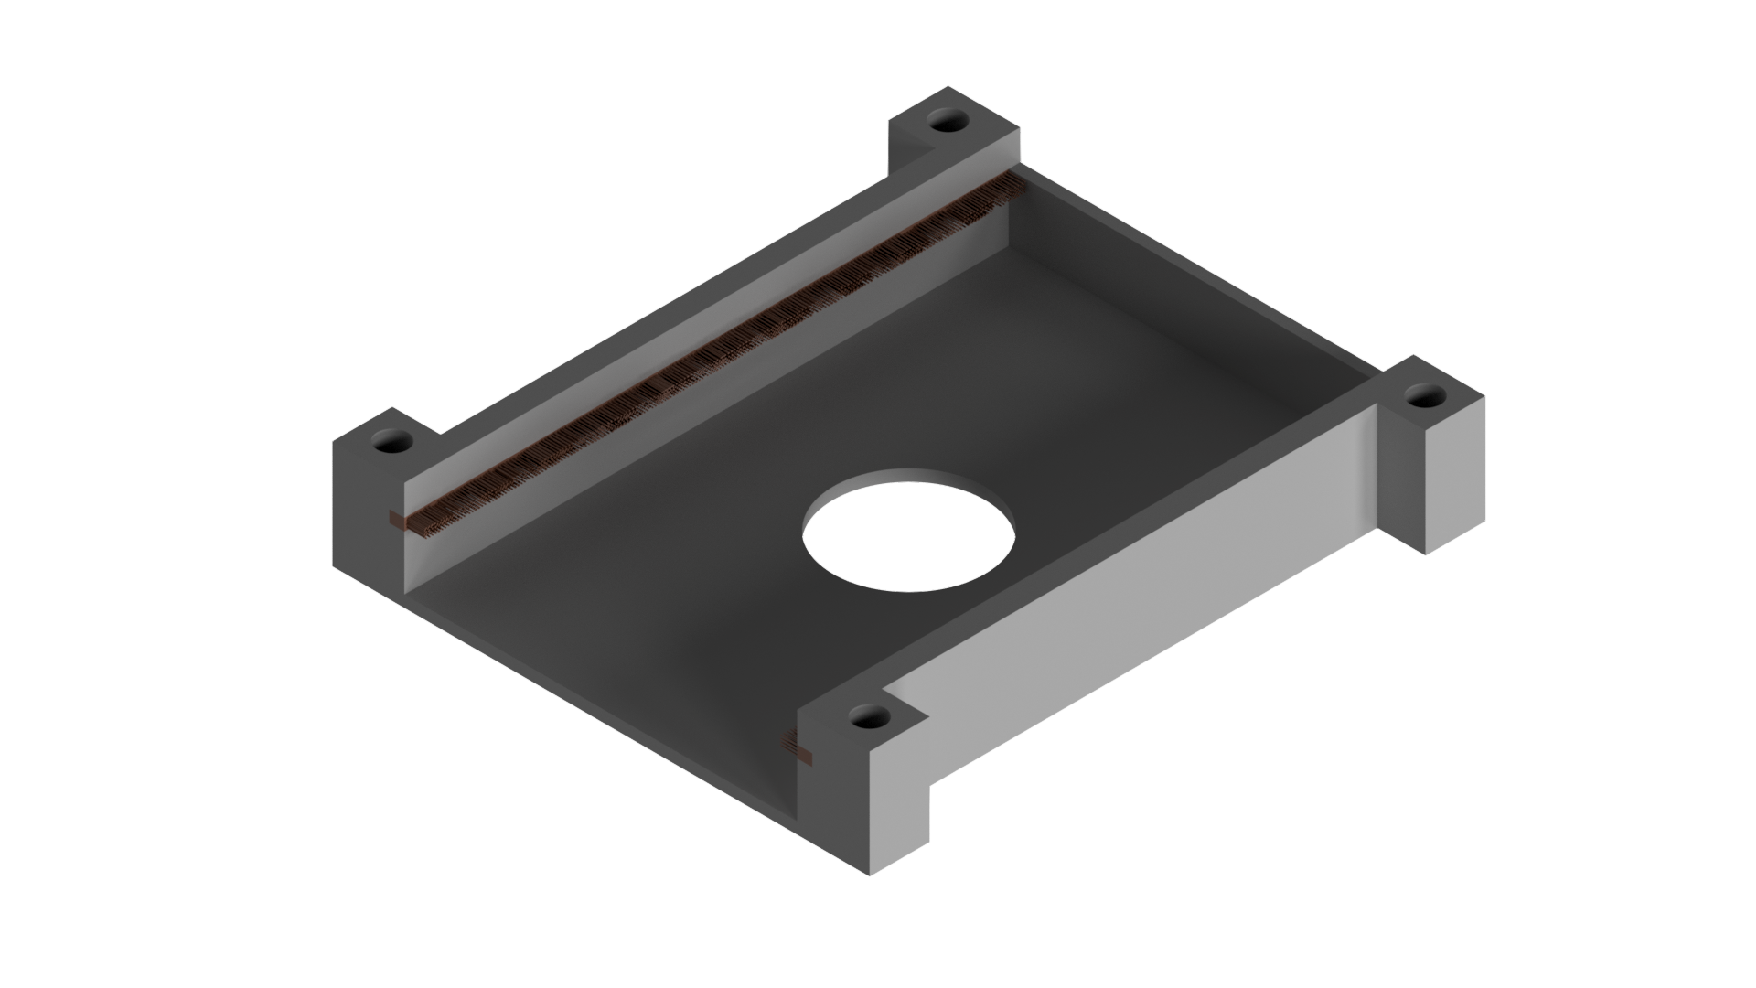
\includegraphics[scale=0.5,page=1]{fig/mech/AusgabeMitBuersten}
        \caption{Ausgabe mit Bürsten}
    \end{figure}

    \item \textbf{Gummiabsstreifer}\\
    Dieses Konzept funktioniert ähnlich wie das Abstreifbürsten-Konzept.
    Es besitzt seitlich Abstreifplatten, die aus Gummi sind.
    Diese sollen der angesaugten Karte helfen, die mitgezogenen Karten abzustreifen.
    Wie beim vorherigen Konzept muss hierbei das Gummi auch so
    dimensioniert werden, dass es einerseits nicht zu steif ist und die eigentlich angesaugte Karte abstreift, andererseits sollte es steif genug sein, um die Karten, die mitgehoben werden abzustreifen.
    Man kann die Steifigkeit des Gummiastreifens verändern, indem man die Breite der Einschnitte
    erhöht oder vermindert.

    \begin{figure}[H]
        \centering
        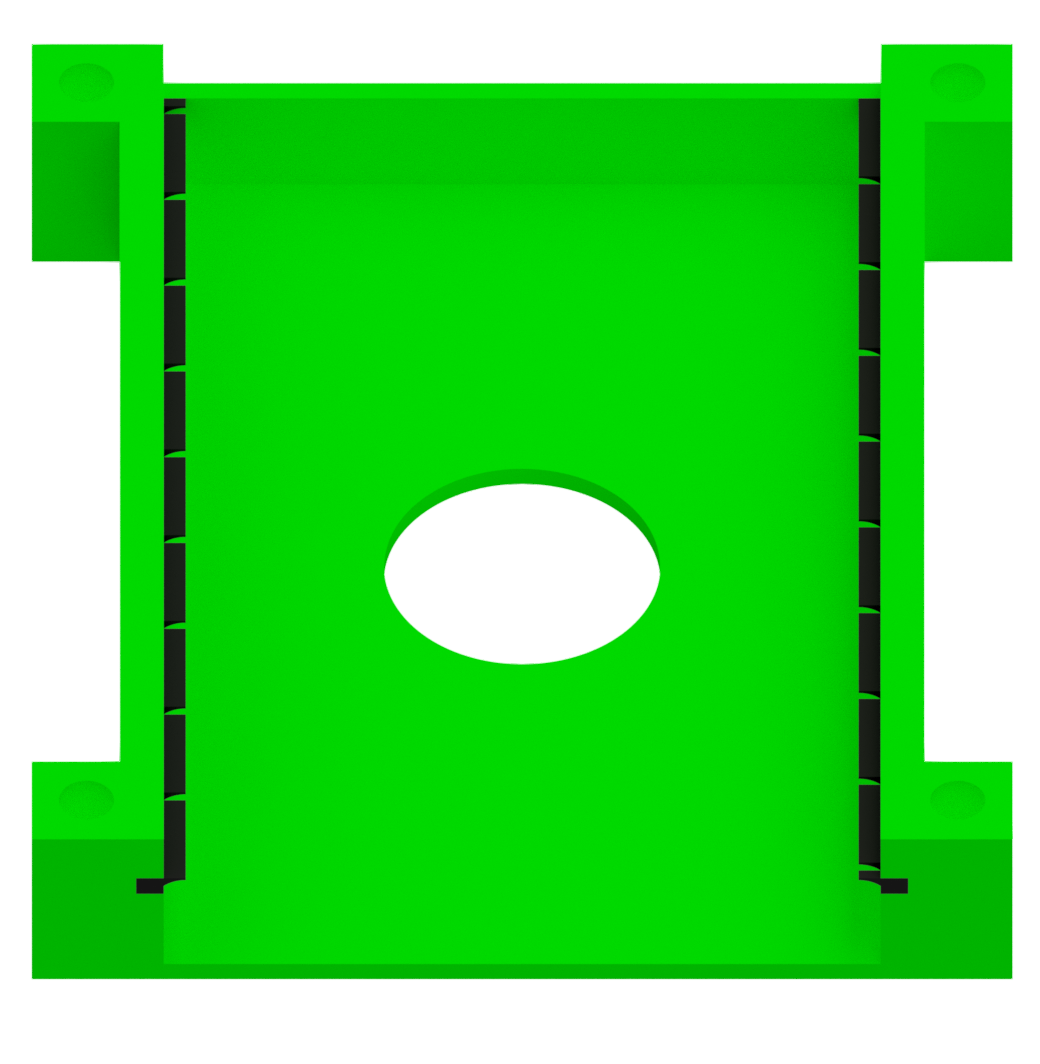
\includegraphics[scale=0.4,page=1]{fig/mech/AsugabeMitGummiabstreifer.png}
        \caption{Ausgabe mit Gummiabsstreifer}
    \end{figure}

    \textbf{Vorteile:}
    \begin{itemize}
        \item Zuverlässig
        \item Billig
    \end{itemize}
    \textbf{Nachteile:}
    \begin{itemize}
        \item Gummi wird spröde
    \end{itemize}
\end{enumerate}

\subsection{Saugmechanismus}

Da bei der 3. Variante Saugnäpfe zum Einsatz kommen, muss entschieden werden, welche Saugnäpfe angewandt werden.

\begin{itemize}
    \item \textbf{Einfacher Unterdruck-Saugnapf} \\
    Die erste Möglichkeit wäre, einen einfachen Saugnapf zu nehmen, der durch Anpressen an eine Oberfläche einen Unterdruck erzeugt und somit haftet.
    Ein Vorteil dieses Saugnapfes ist es, dass dieser kostengünstig ist, keine weiteren Bauteile benötigt sowie eine unkomplizierte Befestigung über ein Gewinde mit sich bringt.
    Jedoch muss dieser Saugnapf mit einer gewissen Kraft auf das Kartendeck gepresst werden, um einen Unterdruck erzeugen zu können.
    Dies kann dazu führen, dass zwischen den Karten auch ein Unterdruck erzeugt wird und somit mehr als eine Karte vom Saugnapf hochgehoben wird.
    Ein weiterer Nachteil wäre, dass die Karte nicht kontrolliert abgeworfen werden kann, da sie erst abfällt, wenn der Unterdruck verschwindet.
    Wenn der Ansaugdruck durch den Hubmagneten nicht erreicht wird, kann es auch dazu führen, dass keine Karte angesaugt wird.
    Dies kann die Wartezeiten wiederum verlängern und somit den Spielablauf stören.

    \textbf{Vorteile:}
    \begin{itemize}
        \item Billig
        \item Unkomplizierter Einbau
    \end{itemize}
    \textbf{Nachteile:}
    \begin{itemize}
        \item Unzuverlässig
    \end{itemize}

    \item \textbf{Vakuumsaugnapf}

    Eine andere Möglichkeit wäre ein Vakuumsaugnapf.
    Dieser erzeugt seinen Unterdruck über eine Vakuumpumpe und kann somit gesteuert werden.
    Der Vorteil dieses Saugnapfes ist es, dass die Karten zu einer gewünschten Zeit abgeworfen werden können, da man den Unterdruck des Saugnapfes durch die Pumpe steuern kann.
    Ein anderer Vorteil ist, dass der Hubmagnet keine hohe Kraft aufweisen muss, da der Saugnapf nicht mehr auf die Karten aufgepresst wird.
    Dies würde auch das Problem, dass mehrere Karten auf einmal aufgehoben werden, lösen.
    Der Nachteil dieser Möglichkeit wäre jedoch der erhöhte Preis des Saugnapfes sowie die zusätzlichen Bauteile, wie zum Beispiel die Pumpe und das Ventil.
    Außerdem ist der Einbau des Saugnapfes etwas komplizierter, da ein Luftdruckschlauch
    zum Saugnapf geführt werden muss.

    \textbf{Vorteile:}
    \begin{itemize}
        \item Zuverlässig
        \item Unterdruck ist kontrollierbar
    \end{itemize}
    \textbf{Nachteile:}
    \begin{itemize}
        \item Mehr Bauteile
        \item Teuer
        \item Komplizierter Einbau
    \end{itemize}
    \pagebreak
    \item \textbf{Vergleich der Saugnäpfe}


    Beide Saugnäpfe würden ihre individuellen Vorteile besitzen.
    Da wir zum einen ein begrenztes Budget haben, wäre der einfache Unterdrucksaugnapf für uns attraktiv, zum anderen wäre der Vakuumsaugnapf durch seine Zuverlässigkeit von Vorteil.
    Da der ausgewählte Hubmagnet jedoch nicht in der Lage ist, den erforderlichen Ansaugdruck zu erreichen,
    und das kontrollierte Abwerfen der Karten maßgeblich für die Funktion der Maschine ist, fällt unsere Auswahl auf den Vakuumsaugnapf.
\end{itemize}

\subsection{Endauswahl der Varianten}

\textbf{\large{Gegenüberstellung der Varianten}}

\begin{table}[H]
    \centering
    \scalebox{0.8}{
    \begin{tabular}{|c|c|c|ll}
        \cline{1-3}
        \textbf{Variante}             & \textbf{Vorteile}                                                                & \textbf{Nachteile}                                                                                    &  &  \\ \cline{1-3}
        1 - Linearachsen              & \begin{tabular}[c]{@{}c@{}}Schnelles Mischen\\ Wenige Fehlerquellen\end{tabular} & \begin{tabular}[c]{@{}c@{}}Teuer\\ Großer Aufbau\\ Instabil\end{tabular}                              &  &  \\ \cline{1-3}
        2 - Lagerrad mit Ausgaberäder & \begin{tabular}[c]{@{}c@{}}Stabil\\ Niedriger Aufbau\end{tabular}                & \begin{tabular}[c]{@{}c@{}}Langes Gehäuse\\ Viele Bewegliche Bauteile / Fehlerquellen\end{tabular} &  &  \\ \cline{1-3}
        3 - Lagerrad mit Saugnäpfe    & \begin{tabular}[c]{@{}c@{}}Billig\\ Wenig bewegliche Bauteile\end{tabular}       & hoher Aufbau                                                                                          &  &  \\ \cline{1-3}
    \end{tabular}}
    \caption{Vergleich der Varianten}
\end{table}

\textbf{\large{Begründung der Wahl}}\\
Alle drei Varianten wurden durchdacht und bieten ihre individuellen Vorteile.
Durch den enormen Preis von Variante 1 ist diese aber nicht für unser Projekt geeignet.
Das optimale Konzept des Mischens wird am besten durch Variante 3 realisiert, da diese die niedrigste Wahrscheinlichkeit aufweist, mehrere Karten auf einmal in das Lager zu befördern.
Da Variante 3 im Vergleich zur Variante 2 weniger Bauteile besitzt, ist diese Variante für uns preislich ansprechend.
Außerdem werden Fehlerquellen durch wenige bewegliche Bauteile minimiert.\\
Somit fällt die finale Wahl auf Variante 3.



\pagebreak
\section{Konstruktion}
\subsection{Konstruktion des Lagerrades}
Das Lagerrad soll durch das zufällige Rotieren das Mischen der Karten ermöglichen.
Im Verlauf der Diplomarbeit wurde das Lagerrad mehrfach überarbeitet.
Die grundsätzliche Form dieses Rades besteht aus einem Viertel eines Hohlzylinders, der in mehrere Fächer unterteilt ist.
Die erste Version dieses Rades besaß 20 Unterteilungen.

\begin{figure}[H]
    \centering
    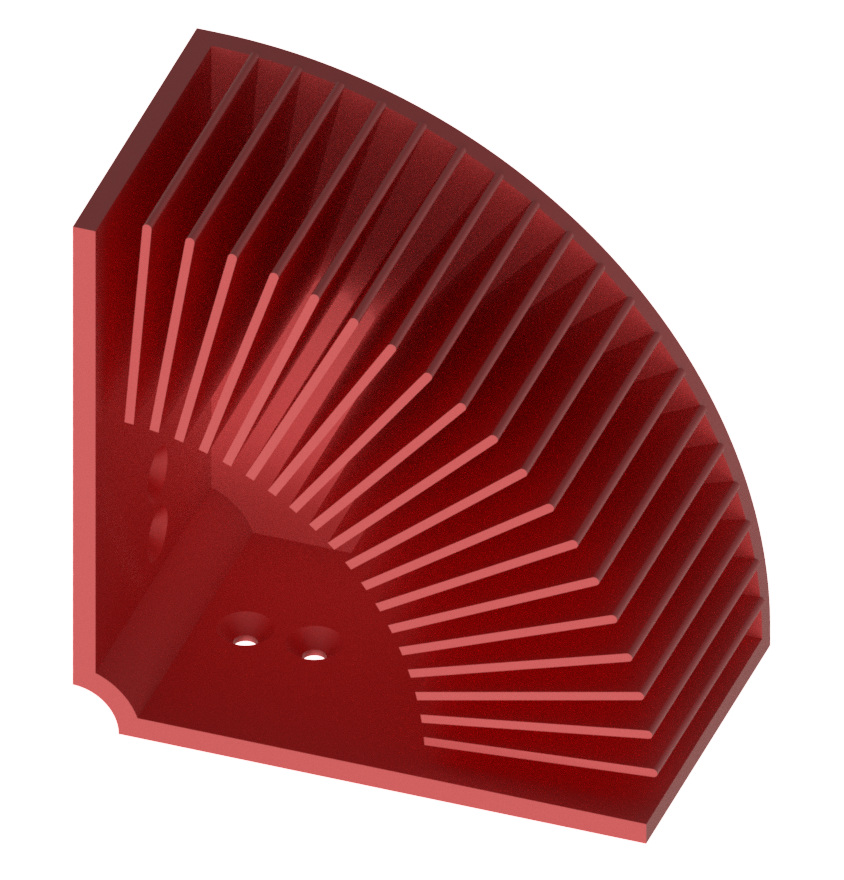
\includegraphics[scale=0.5,page=1]{fig/mech/LagerRad}
    \caption{Version 1: Lagerrad 20 Fächer (geöffnete Außenwand zur vereinfachten Ansicht)}
    \label{fig:Lagerrad 20 Fächer}
\end{figure}
In der \autoref{fig:Lagerrad 20 Fächer} wurde die Außenwand entfernt, um eine bessere Einsicht in das Bauteil zu bekommen.
Durch die 20 Unterteilungen muss der Schrittmotor genauere Positionen anfahren, außerdem wäre der Aufwand beim Produzieren groß.
Aus diesem Grund entschieden wir uns, die Unterteilungen zu minimieren und kamen zu dem Entschluss, dass vier Unterteilungen für ein optimales Mischen ausreichen.
Diese Konstruktion wurde nach einem Stecksystem entworfen, sodass man die einzelnen Teile herstellen kann und diese danach zusammenstecken und verkleben kann.

\begin{figure}[H]
    \centering
    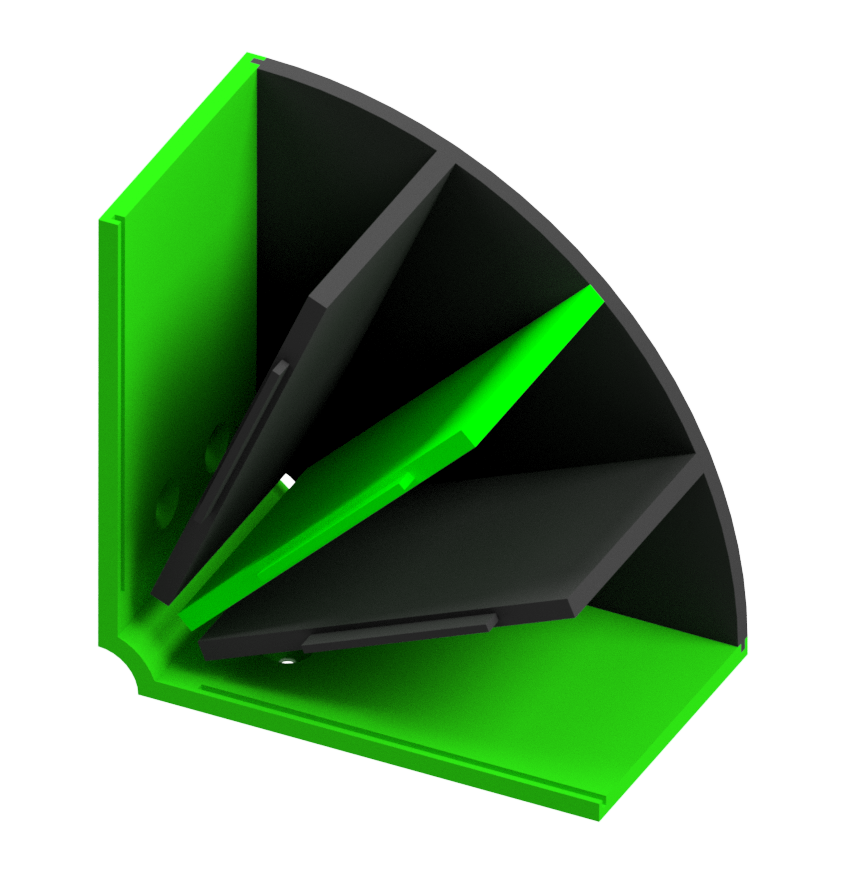
\includegraphics[scale=0.5,page=1]{fig/mech/LagerradSingle}
    \caption{Version 2: Lagerrad 4 Fächer (geöffnete Außenwand zur vereinfachten Ansicht)}
    \label{fig:Lagerrad 4 Fächer}
\end{figure}


In der \autoref{fig:Lagerrad 4 Fächer} wurde die Außenwand entfernt, um das Bauteil besser zu veranschaulichen.
Das Lagerrad besteht aus mehreren Einzelteilen:

\subsubsection{Außenwände}
Die Außenwände wurden in der Form eines Teiles eines Kreises konstruiert und geben somit die Form des Lagerrades vor.
Sie besitzen jeweils zwei Laschen an der äußeren Seite.
Diese verbinden die Außenwände später mit den Seitenwänden des Lagerrades.
Außerdem besitzen sie jeweils drei Ausfräsungen auf ihrer Grundfläche, über die sie später mit den Trennplatten versteckt werden.
Bei der Konstruktion der Ausfräsungen ist dabei zu achten, dass sie etwas größer als benötigt gezeichnet werden, da bei der
Fertigungsart des 3D-Druckens Innenbohrungen und Innenfräsungen durch die Ungenauigkeit des Druckers kleiner gedruckt werden.
Wie auch bei Innenfräsungen müssen die Laschen auf der Außenseite etwas kleiner konstruiert werden, da diese widerum beim
Drucken größer gedruckt werden, als sie ursprünglich gezeichnet wurden.

\subsubsection{Seitenwände}
Diese Bauteile verbinden das Lagerrad mit dem Lagerradhalterungsmodul.
Sie besitzen auf der äußeren Seite der Grundfläche jeweils zwei Auskerbungen.
Über diese werden sie mit den Laschen der Außenwände verbunden.
Um einen Durchgang für die Welle zu schaffen, schließen die Bauteile auf der unteren Seite nicht im rechten Winkel ab, sondern sind nach innen radial abgerundet.
Je Bauteil sind zwei Bohrungen vorhanden, über welche es mit dem Lagerradhalterungsmodul verbunden wird.
Die Bohrungen sind als Senklochbohrungen ausgeführt, da somit die Schraube komplett in das Bauteil versenkt werden kann
und das Hineinrutschen der Karten in das Lagerrad nicht behindert wird.

\subsubsection{Trennplatte}
Um die einzelnen Lagerfächer zu unterteilen, ist die Trennplatte konstruiert worden.
Dieses Bauteil ist ein einfacher Quader mit je zwei Laschen an den Außenseiten.
Diese Laschen werden mit den Ausfräsungen der Außenplatte versteckt.
Hierbei ist wieder zu achten, dass die Laschen kleiner konstruiert werden, da sie durch den 3D-Druck an Größe zunehmen .

\subsection{Konstruktion des Lagerradhalterungsmoduls}
\begin{wrapfigure}{r}{8 cm}
    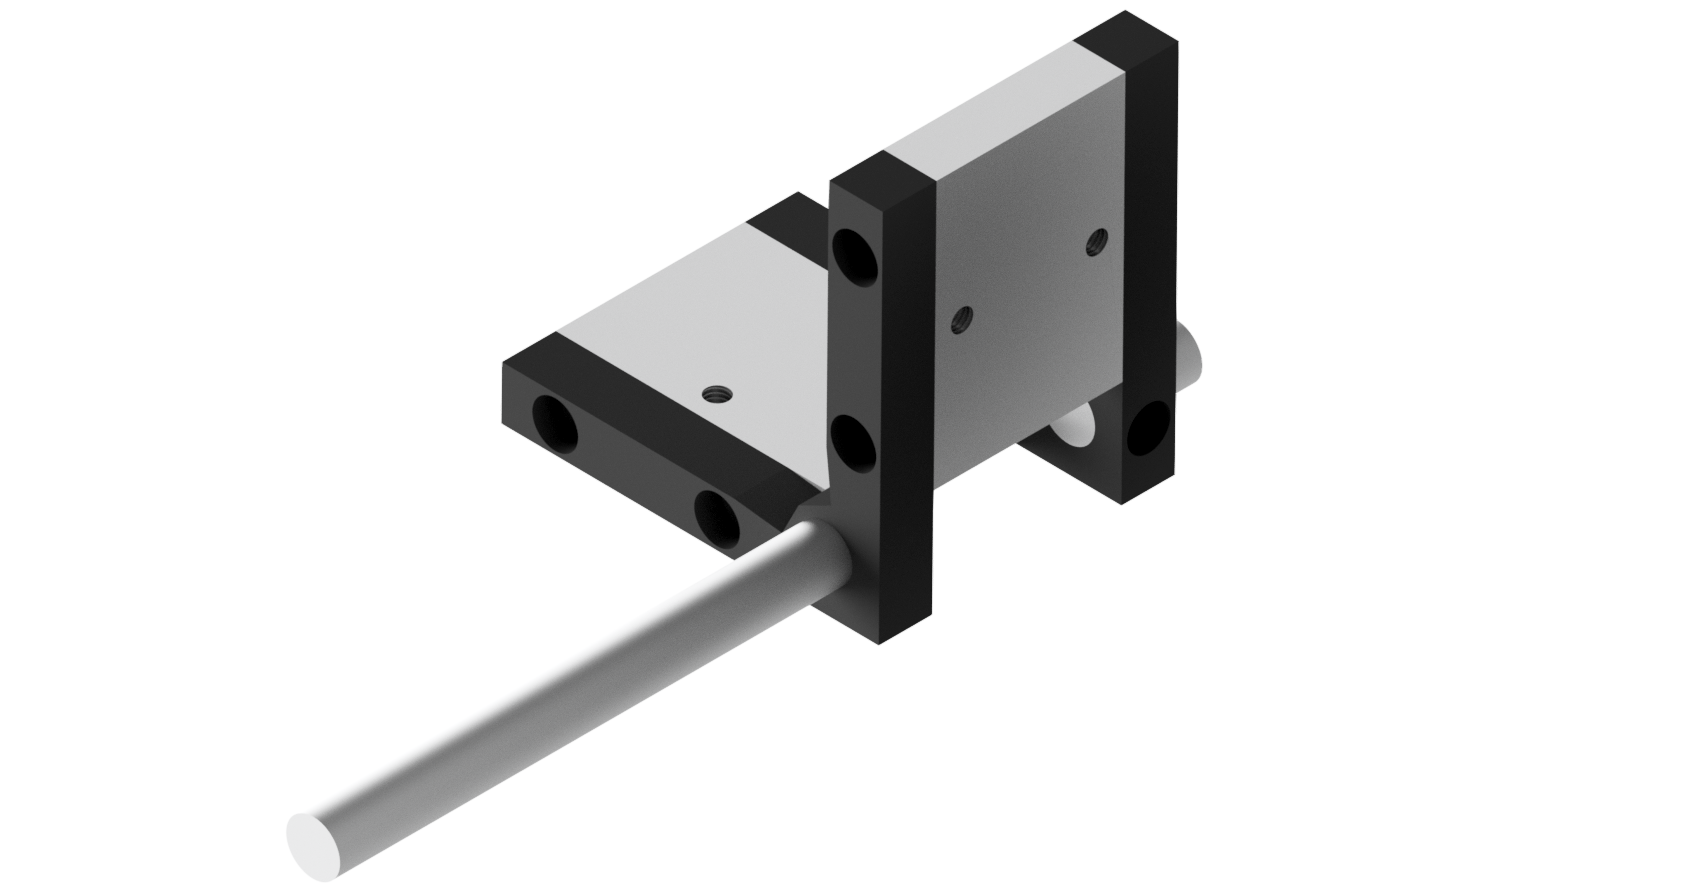
\includegraphics[width=8 cm]{fig/mech/LagerRadGruppekomplett}
    \caption{Lagerradhalterungsmodul}
    \label{fig:Lagerradhalterungsmoduls}
\end{wrapfigure}
Um das Moment der Welle effektiv von der Welle zum Rad zu übertragen, wurde ein Lagerradhalterungsmodul (\autoref{fig:Lagerradhalterungsmoduls}) entworfen.
Dieses Modul wird benötigt, da das Wellenmoment nicht effektiv an einem 3D-gedruckten Bauteil angreifen kann, weil das gedruckt PLA
die kontinuierlichen Richtungswechsel sowie das abrupte Bremsens des Motors in Kombination mit der
Trägheit des Lagerrades nicht standhalten würde.
Dieses Modul besteht aus folgenden Einzelteilen:

\subsubsection{L-Grundplatte}
\begin{wrapfigure}{r}{8 cm}
    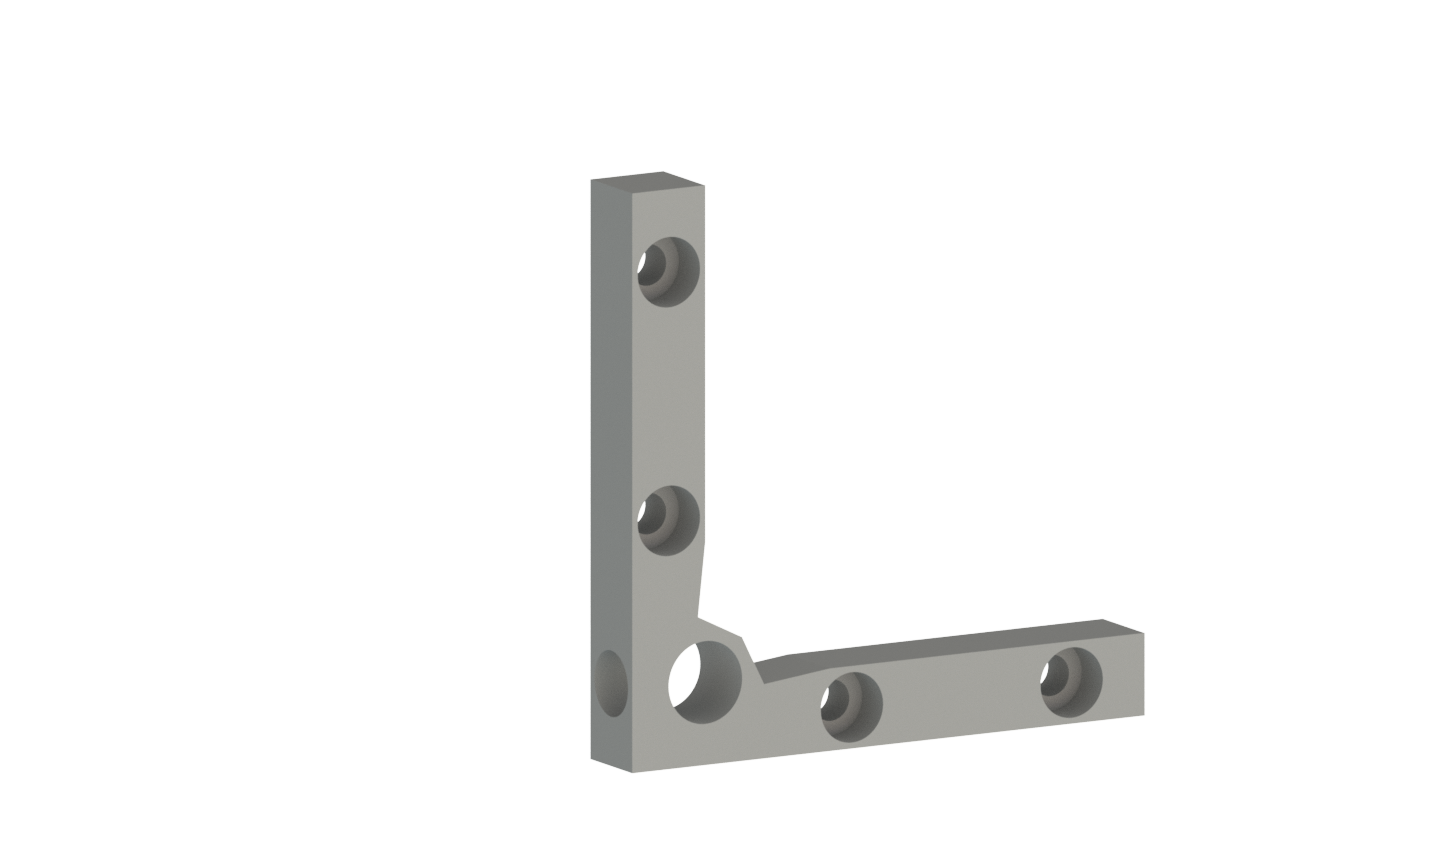
\includegraphics[width=8 cm]{fig/mech/L_Grundplatte}
    \caption{L-Grundplatte}
    \label{fig:L-Grundplatte}
\end{wrapfigure}
Dieses Bauteil, siehe \autoref{fig:L-Grundplatte}, verbindet die Motorwelle sowie die Lagerwelle mit der Verbindungsplatte und somit auch das Lagerrad.
Es überträgt zusätzlich auch das Moment des Motors.
Das Bauteil besitzt je vier Bohrungen mit Zylinderschraubensenkungen, über die sie mit
der Verbindungsplatte verbunden wird.
Außerdem besitzt sie eine Bohrung mit einer Querbohrung.
Über diese werden die Wellen geführt und mit einer Schraube am Bauteil fixiert.
Dieses Bauteil wurde ursprünglich aus Aluminium gefertigt, durch Versuche mit einer 3D-gedruckten L-Grundplatte zeigte
sich jedoch, dass diese sich genauso gut eignet und optisch ansprechender ist.
Um nicht in Konflikt mit dem Lagerrad zu stehen, hat das Bauteil jeweils zwei Ausbuchtungen nahe der Welle.

\subsubsection{Verbindungsplatte}
\begin{wrapfigure}{r}{8 cm}
    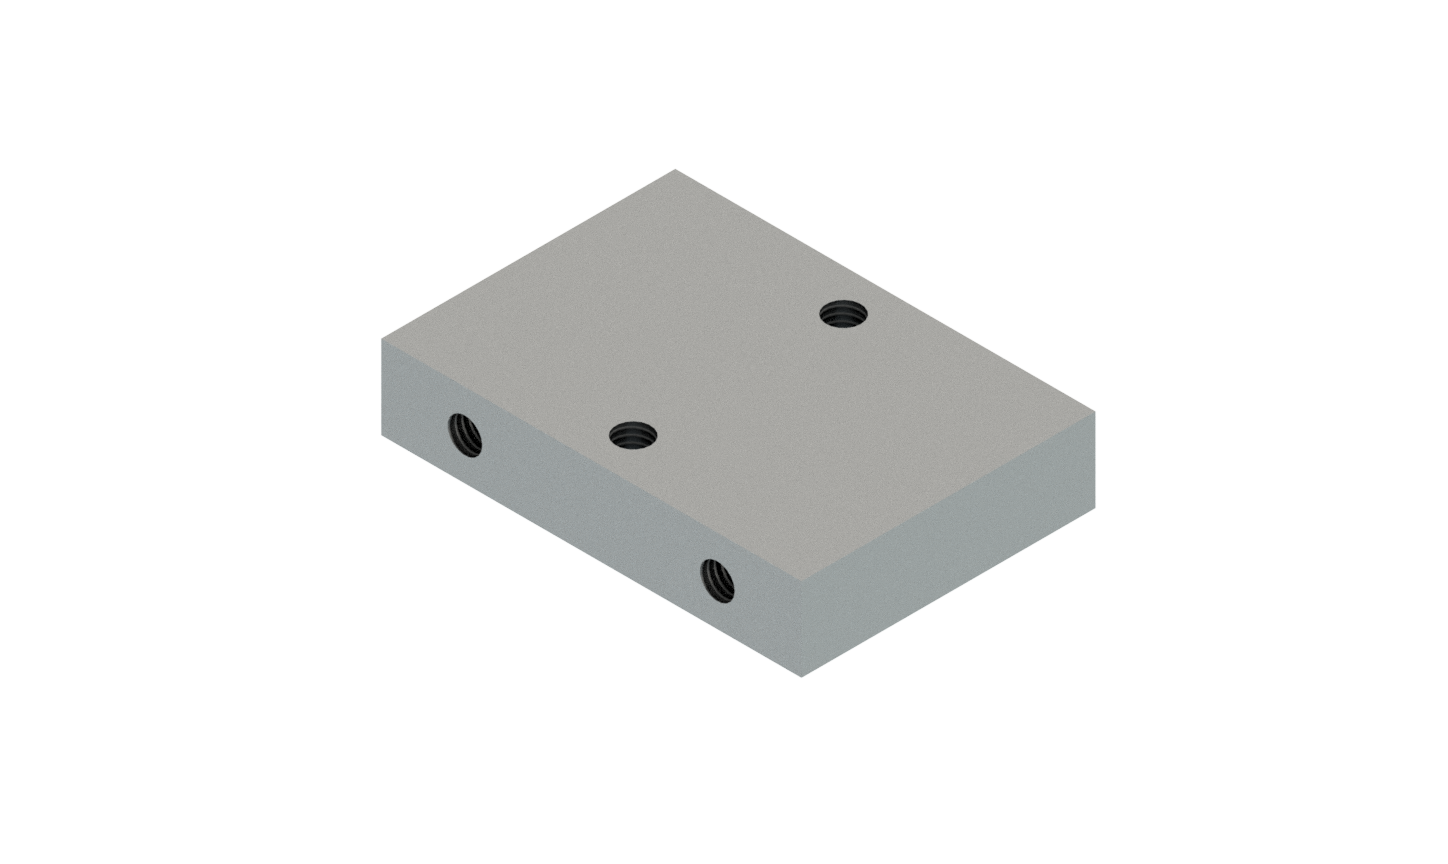
\includegraphics[width=8 cm]{fig/mech/Verbindungsplatte}
    \caption{Verbindungsplatte}
    \label{fig:Verbindungsplatte}
\end{wrapfigure}
Die Verbindungsplatte, zu sehen in \autoref{fig:Verbindungsplatte}, nimmt das von der L-Grundplatte aufgenommene Moment des Motors und überträgt es an das Lagerrad weiter.
Sie wurde als einfacher Aluminiumquader konstruiert und besitzt insgesamt sechs Bohrungen.
Zwei Bohrungen sind auf der Grundfläche des Bauteils und besitzen ein Gewinde.
Diese verbinden das Lagerradhalterungsmodul mit dem Lagerrad.
Je zwei Bohrungen sitzen auf der Unterseite sowie auf der Oberseite der Verbindungsplatte und sind ebenfalls mit Gewinde
ausgeführt, durch diese Gewindebohrungen wird das L-Bauteil mit der Verbindungsplatte verbunden.
Dieses Bauteil wurde aus Aluminium gefertigt, da es problematisch ist ein Gewinde in PLA zu schneiden, außerdem spielt
das zusätzliche Gewicht des Aluminiums bei diesem Modul nur eine geringe Rolle.

\subsubsection{Motorwelle}
\begin{wrapfigure}{r}{8 cm}
    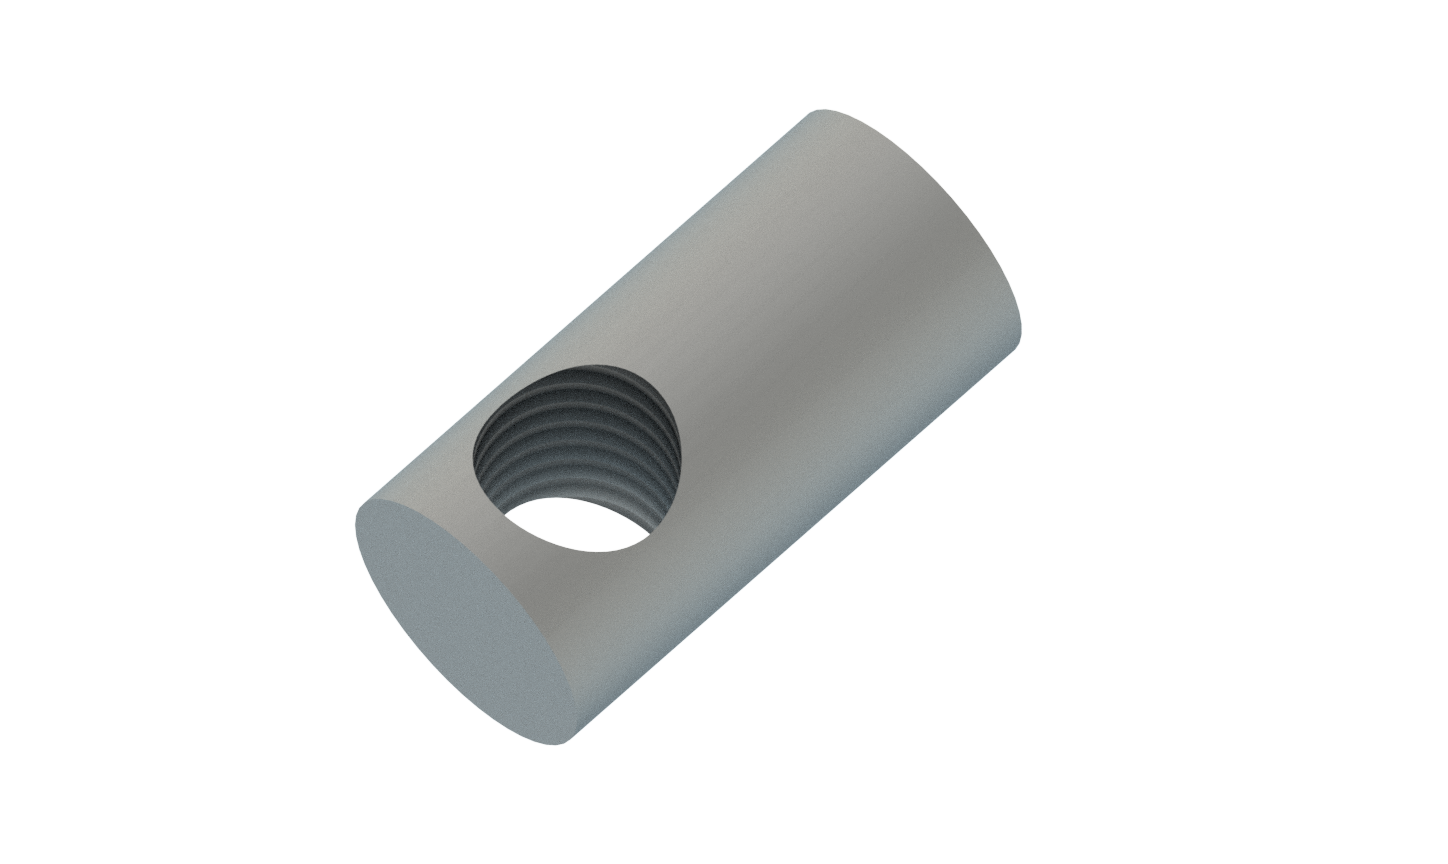
\includegraphics[width=8 cm]{fig/mech/Motorwelle.png}
    \caption{Motorwelle}
    \label{fig:Motorwelle}
\end{wrapfigure}
Um das Moment vom Motor auf die L-Grundplatte zu übertragen, wird die Motorwelle, die in \autoref{fig:Motorwelle} zu sehen ist, benötigt.
Das Bauteil ist eine einfache Welle mit einer Gewindebohrung am äußeren Ende der Welle.
Diese dient dazu, die Welle mit der L-Grundplatte zu verbinden.
Am anderen Ende ist die Welle über die Kupplung mit dem Motor verbunden.
Die Welle wurde an der Drehbank gefertigt und anschließend an der Fräsmaschine die Gewindebohrung gebohrt.

\pagebreak
\subsubsection{Lagerwelle}
\begin{wrapfigure}{r}{8 cm}
    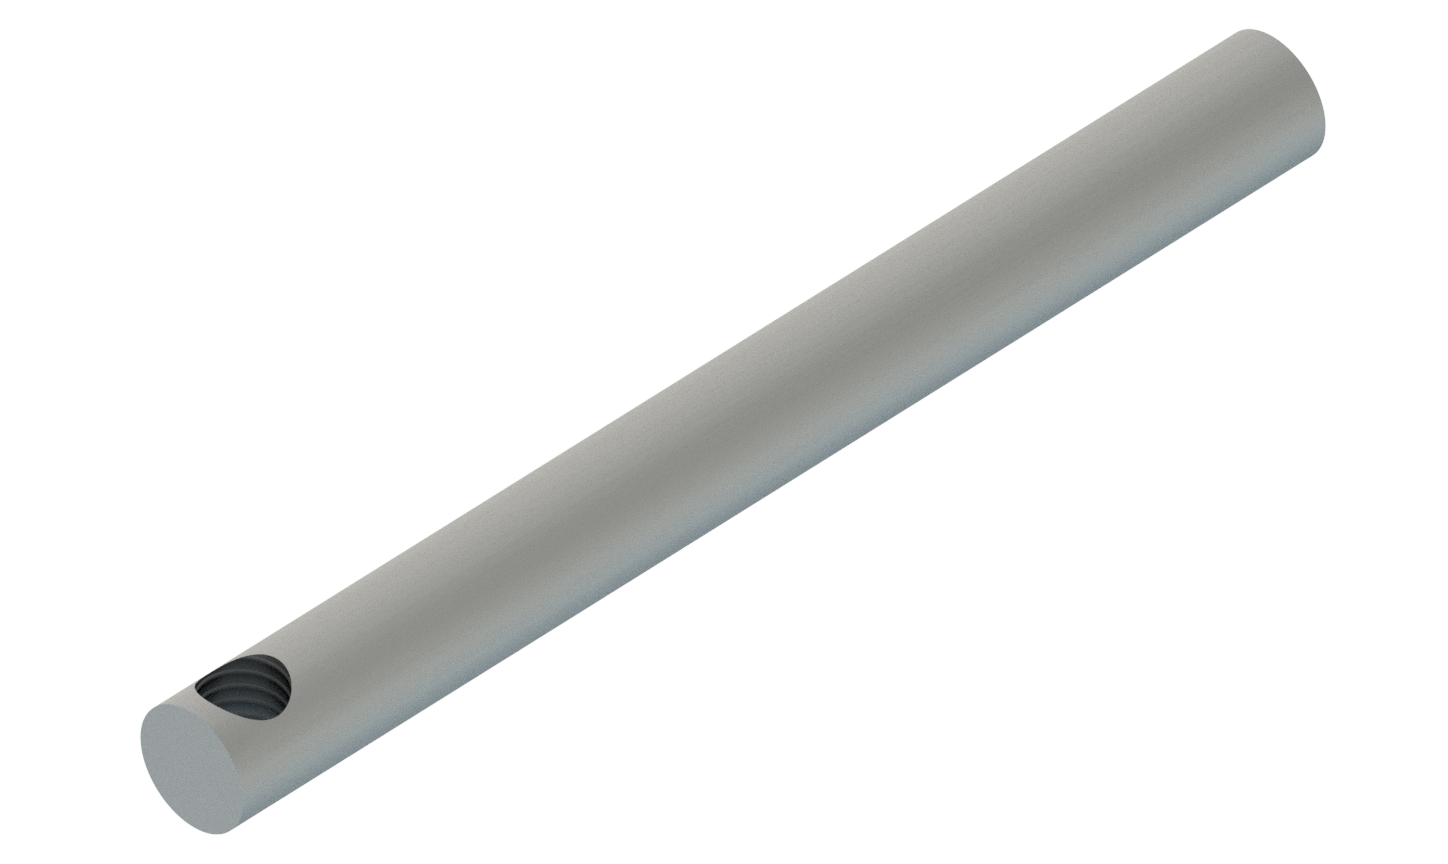
\includegraphics[width=8 cm]{fig/mech/Lagerwelle.png}
    \caption{Lagerwelle}
    \label{fig:Lagerwelle}
\end{wrapfigure}

Die Lagerwelle unterscheidet sich von der Motorwelle lediglich durch ihre Länge.
Sie wird auf der einen Seite mit der L-Grundplatte verschraubt, auf der anderen Seite wird sie mit dem Zweiloch-Flanschlager auf der Vorderseite des Gehäuses über
zwei Wurmschrauben geklemmt.
Abgebildet ist diese in \autoref{fig:Lagerwelle}.\\




\subsection{Konstruktion der Motorhalterungsgruppe}


Die Motorhalterung, siehe \autoref{fig:SchrittmotorCombinedWinkel}, hat den Zweck, den Motor an das Gehäuse zu befestigen und ihn somit für die Welle auszurichten.
Der ausgewählte Schrittmotor besitzt eine mitgelieferte Montagehalterung, die mit vier Schrauben an den Motor geschraubt wird.
Die Motorhalterung entspricht dem Nema 17 Standard und ist somit universal für Motoren dieser Norm anwendbar.
Die Motorhalterung wird mittels 2 Schrauben an einen verzinkten Edelstahlwinkel angeschraubt, ist aber in der Position noch einrichtbar.
Der Winkel wird über vier Schrauben mit dem Gehäuse aus Polycarbonat verschraubt. \\

\begin{figure}[H]
    \centering
    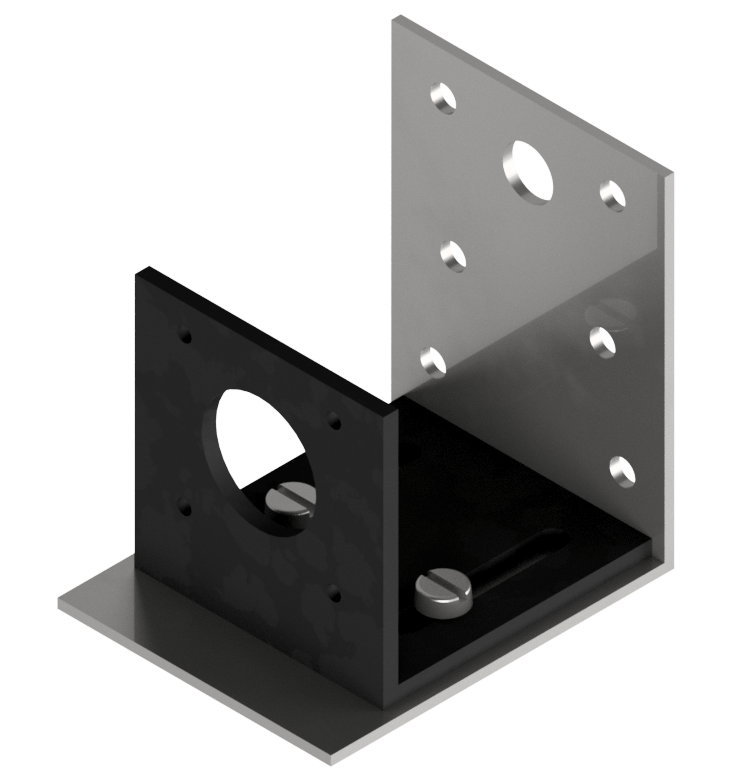
\includegraphics[width=6 cm]{fig/mech/SchrittmotorCombinedWinkel}
    \caption{Motorhalterunsgruppe}
    \label{fig:SchrittmotorCombinedWinkel}
\end{figure}

\subsection{Konstruktion des Kartenhalterungsmodul}
\begin{figure}[H]
    \centering
    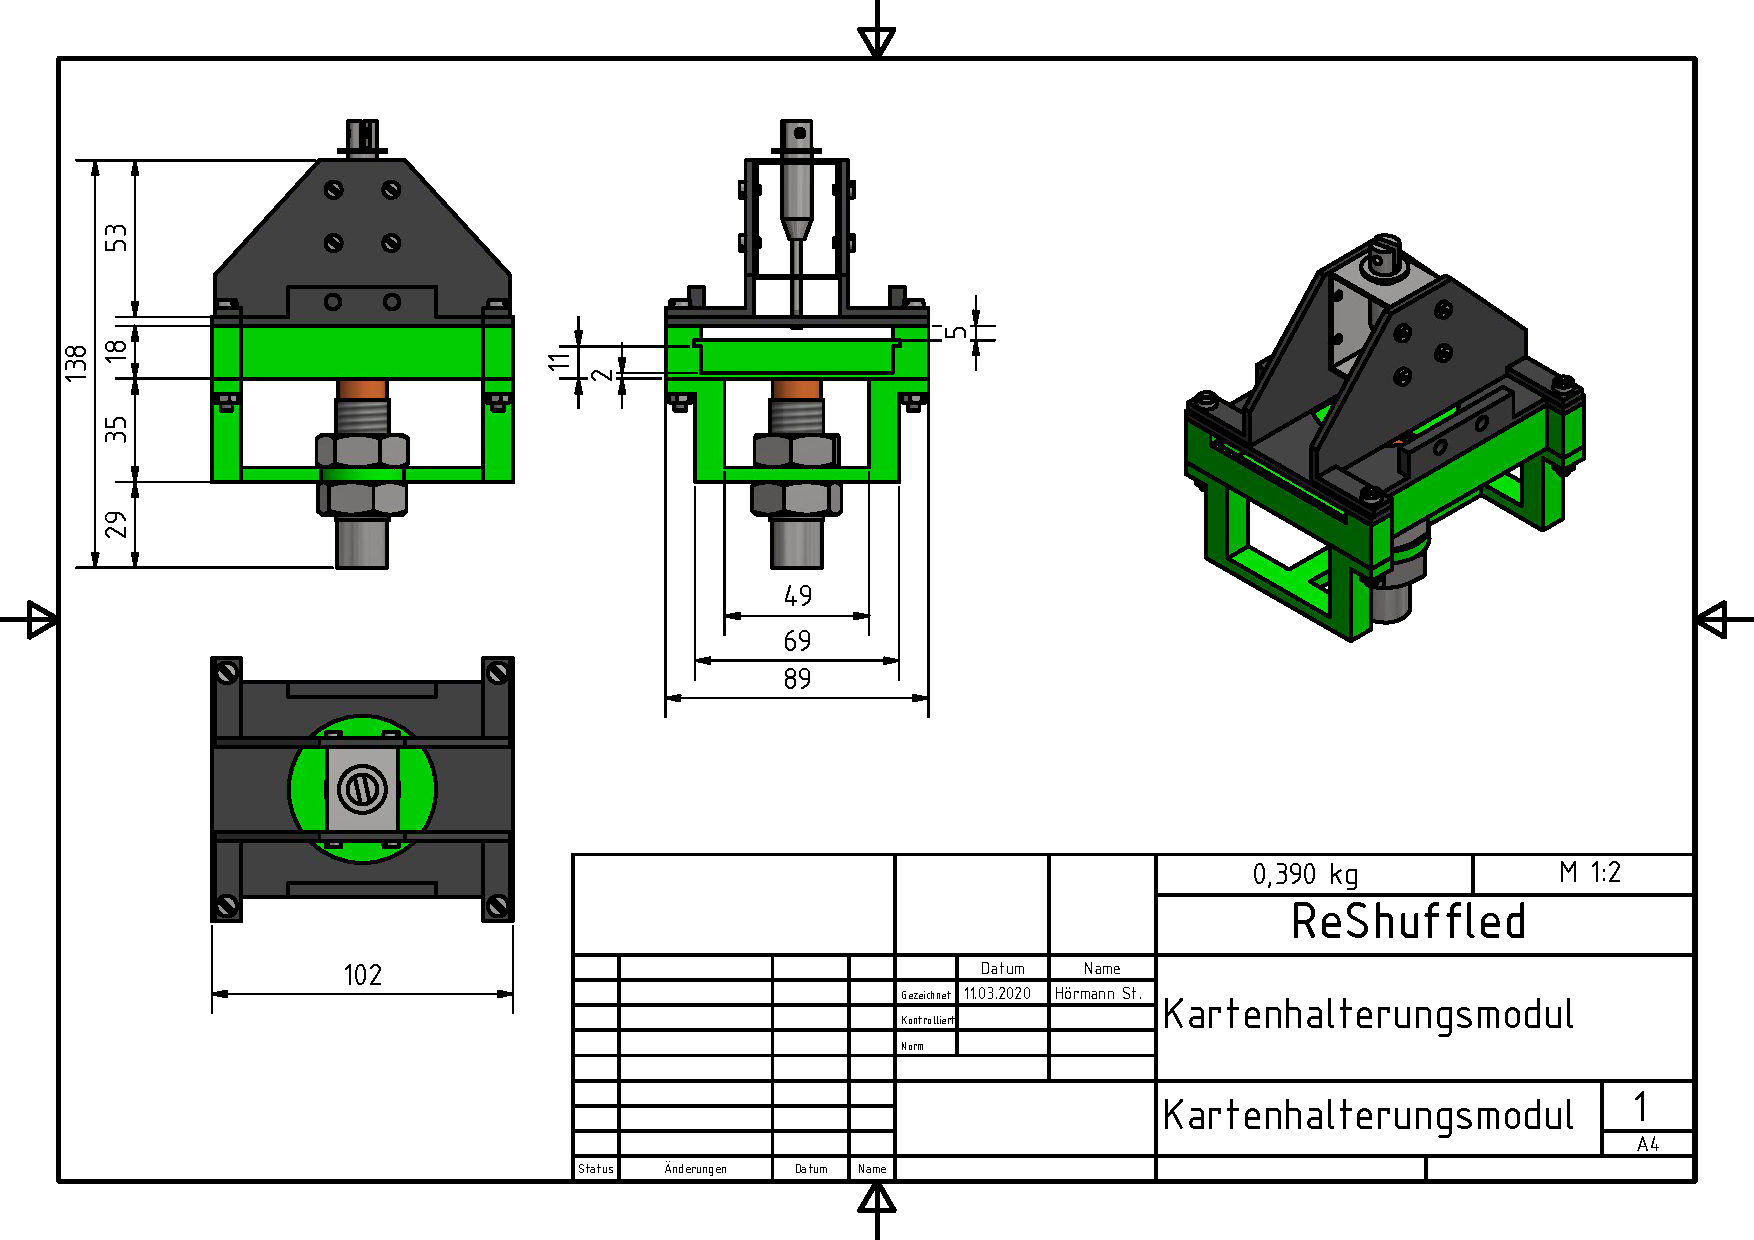
\includegraphics[width=7 cm]{fig/mech/Kartenhalterungsmodul}
    \caption{Kartenhalterungsmodul}
    \label{fig:Kartenhalterungsmodul}
\end{figure}
Die Karten müssen nach dem Einführen in die Maschine und nach dem Auswerfen aus dem Lagerrad zwischengelagert werden, da sie von dem Hubmagneten und dem Saugnapf einzeln aufgehoben und ausgegeben werden.
Für diese Aufgabe kommt das Modul der Kartenhalterung, siehe \autoref{fig:Kartenhalterungsmodul}, zum Einsatz.
Dieses Modul muss sicherstellen, dass genug Platz für mindestens 20 gewöhnliche Spielkarten  mit den Maßen 100 x 66 vorhanden ist.
Das Modul besteht aus mehreren einzelnen Bauteilen:



\subsubsection{Sensorhalterung}

Die Sensorhalterung, siehe \autoref{fig:Sensorhalterung}, dient dazu, den kapazitiven Sensor zu befestigen.
Dieser wird mithilfe von zwei Muttern und zwei Sicherungsringen über das Gewinde des Sensors befestigt.
Durch diese spezielle Befestigungsart kann man den Sensor in der Höhe einrichten und ihn so auf andere Bauteile abstimmen.
Die Sensorhalterung wird über vier Bohrungen mit dem Kartenlager verschraubt.
\begin{figure}[H]
    \centering
    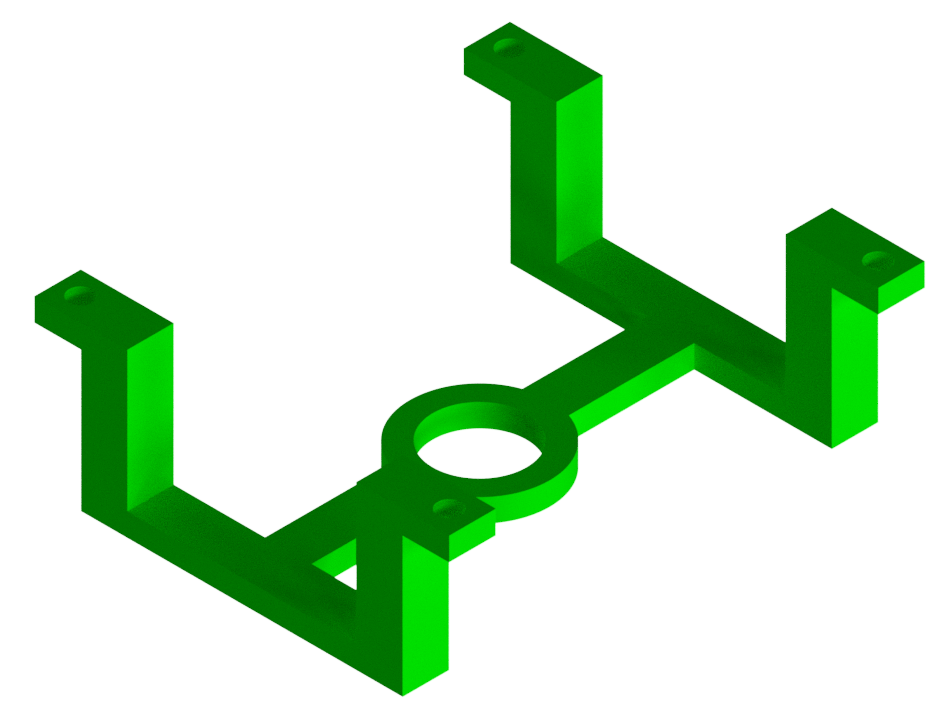
\includegraphics[width=8 cm]{fig/mech/SensorhalterungNeu.png}
    \caption{Sensorhalterung}
    \label{fig:Sensorhalterung}
\end{figure}


\subsubsection{Kartenlager}

Um 20 Karten zwischenzulagern wird ein Kartenlager, das in \autoref{fig:Kartenlager} zu sehen ist, benötigt.
Dieses Lager hat eine Öffnung auf der oberen Seite in der die Karten eingeführt werden.
Auf der unteren Seite liegt es eine Öffnung, die Platz für eine Karte zum Herausfallen bietet.
Diese Öffnung ist auf einer Höhe von 11 mm, sodass die eingelagerten Karten nicht selbständig herausfallen, sondern erst durch das Heben des Hubmagnetes.\\
\begin{wrapfigure}{r}{8 cm}
    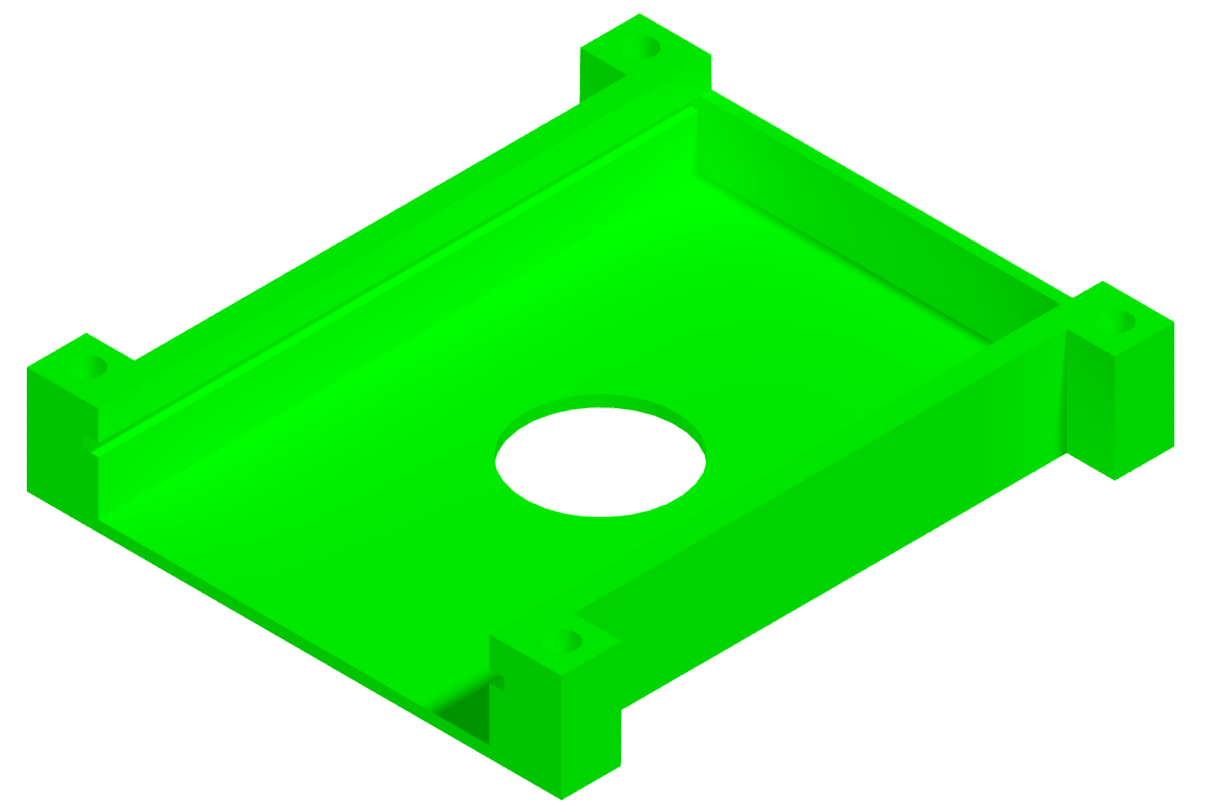
\includegraphics[width=8 cm]{fig/mech/Kartenhalterung}
    \caption{Kartenhalterung}
    \label{fig:Kartenlager}
\end{wrapfigure}
Das Kartenlager besitzt außerdem zwei Einkerbungen in einer Höhe von 11 mm auf den Seiten.
Diese bieten Platz für einen Gummiabstreifer, dessen Funktion ist es, mehrerer auf einmal aufgehobene Karten zu trennen und somit sicherzustellen, dass nur eine Karte ausgegeben wird.
Der Gummiabstreifer stellt auch sicher, dass die Karte aus der Kartenhalterung herausgeworfen wird und nicht wieder zurück auf den Kartenstapel
fällt. \\
Das Lager besitzt außerdem eine runde Ausnehmung auf der Unterseite, durch diese Ausnehmung wird der Sensor geführt und so eingestellt,
dass er plan mit der Grundfläche des Lagers ist.
Die Ausnehmung ist auch so konstruiert, dass sie groß genug ist um vom Sensor nicht erkennt zu werden, wenn dieser auf seiner maximalen Sensibilität konfiguriert ist.\\
Verbunden ist das Kartenlager über vier Schrauben mit dem Abstreifer und der Sensorhalterung.



\subsubsection{Abstreifer}
\begin{wrapfigure}{r}{8 cm}
    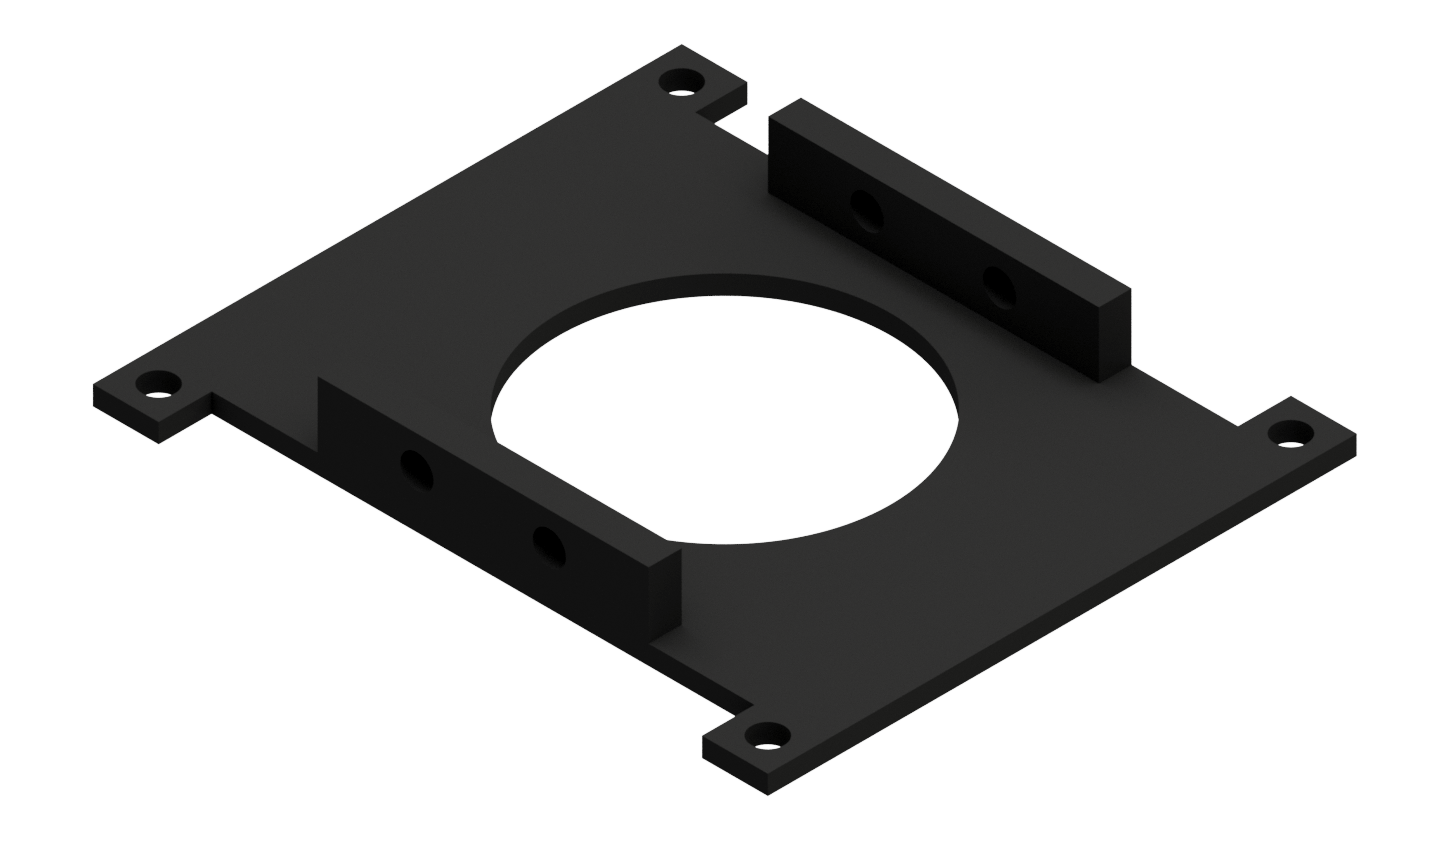
\includegraphics[width=8 cm]{fig/mech/Abstreifer}
    \caption{Abstreifer}
    \label{fig:Abstreifer}
\end{wrapfigure}
Der Abstreifer, siehe \autoref{fig:Abstreifer}, dient dazu, Karten die nicht durch das Lösen des Unterdrucks vom Saugnapf fallen und noch an ihn haften,
abzuwerfen.
Er ist so konstruiert, dass er beim Einfahren des Hubmagnetes die Karten leicht berührt und diese somit vom
Saugnapf löst.
Er besitzt eine Öffnung auf der Grundfläche, die groß genug für unseren ausgewählten Saugnapf ist.\\
Seitlich besitzt das Bauteil zwei Erhebungen mit jeweils zwei Durchbohrungen, über diese wird das gesamte Modul über jeweils 2 Aufhänger
mit dem Gehäuse verschraubt. \\
Der Abstreifer wird durch vier Schrauben mit dem Kartenlager und mit der Hubmagnetaufhängung verbunden.



\subsubsection{Hubmagnetaufhängung}
\begin{wrapfigure}{r}{8 cm}
    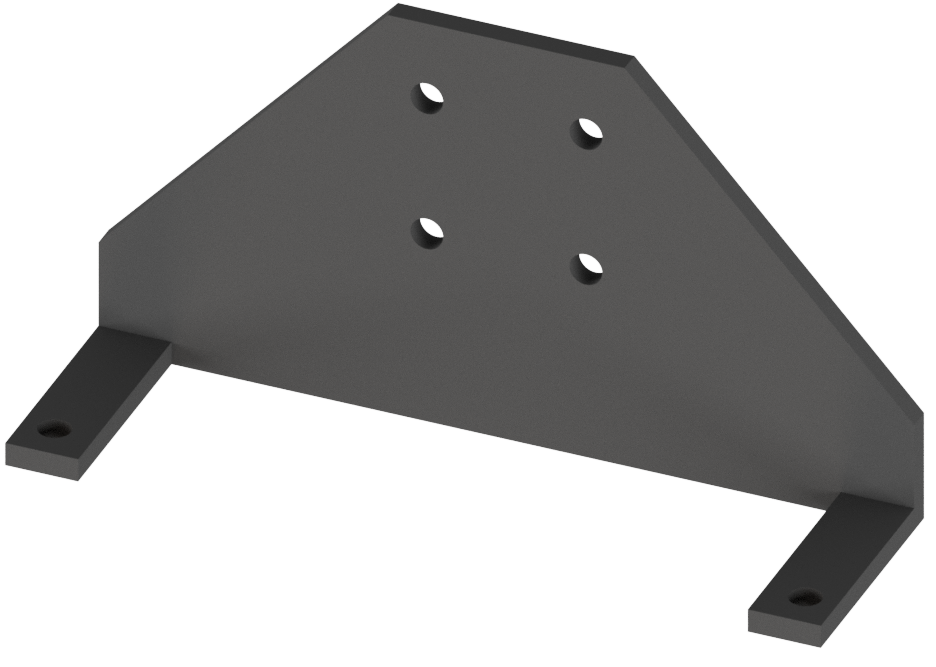
\includegraphics[width=8 cm]{fig/mech/AufhaengungHubmahgnet}
    \caption{Hubmagnetaufhängung}
    \label{fig:Hubmagnetaufhängung}
\end{wrapfigure}
Die Hubmagnetaufhängung, siehe \autoref{fig:Hubmagnetaufhängung}, besteht aus zwei symmetrischen Bauteilen.
Diese Bauteile, welche die Form eines Trapezes besitzen, fixieren den Hubmagneten mit jeweils vier Schrauben pro Seite auf seiner Position.
Das Bauteil ist so konstruiert, dass der ausgefahrene Hubmagnet mit dem montierten Saugnapf die Grundfläche des Kartenlagers erreicht, und somit in der Lage ist,
alle Karten anzusaugen.\\
Die Aufhängung ist mit jeweils zwei Bohrungen mit dem Abstreifer verschraubt und somit an dem gesamten Modul befestigt.



\subsubsection{Aufhänger}
Um das Modul in die gewünschte Position zu bringen werden Aufhänger benötigt, diese sind mit dem Polycarbonatsgehäuse verschraubt.
Da die Aufhänger keinen Krafteinwirkungen ausgesetzt sind, können diese dünn und materialsparend konstruiert werden.
Da das Kartenhalterungsmodul zweimal an verschiedenen Position zum Einsatz kommt, wurden zwei unterschiedliche
Aufhänger konstruiert.\\\\
\textbf{Aufhänger Oben:} \\
\begin{figure}[H]
    \centering
    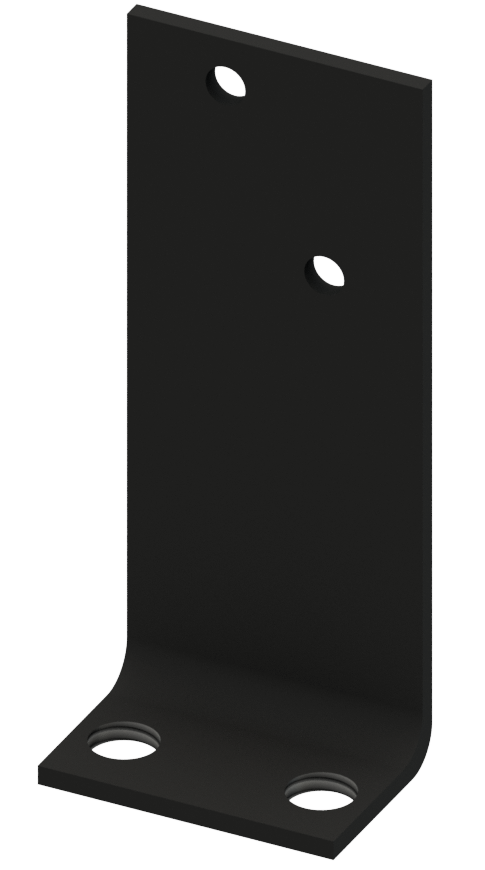
\includegraphics[scale = 0.2]{fig/mech/StopperObenKurz.png}
    \caption{Aufhänger Oben}
    \label{fig:Aufhänger Oben}
\end{figure}
Dieser Aufhänger, siehe \autoref{fig:Aufhänger Oben}, wird über jeweils zwei Schrauben an der Topplatte des Gehäuses befestigt und hält das obere Kartenhalterungsmodul in Position.
Das Modul wird über zwei versetzte Bohrungen mit dem Aufhänger verschraubt.
Diese sind so konstruiert, dass das Modul in einem Winkel von 60° befestigt wird.
Durch die niedrige Höhe des Aufhängers ist auch trotz der dünnen Bauweise genug Stabilität gegeben.\\\\


\textbf{Aufhänger Unten:}

\begin{wrapfigure}{r}{8cm}
    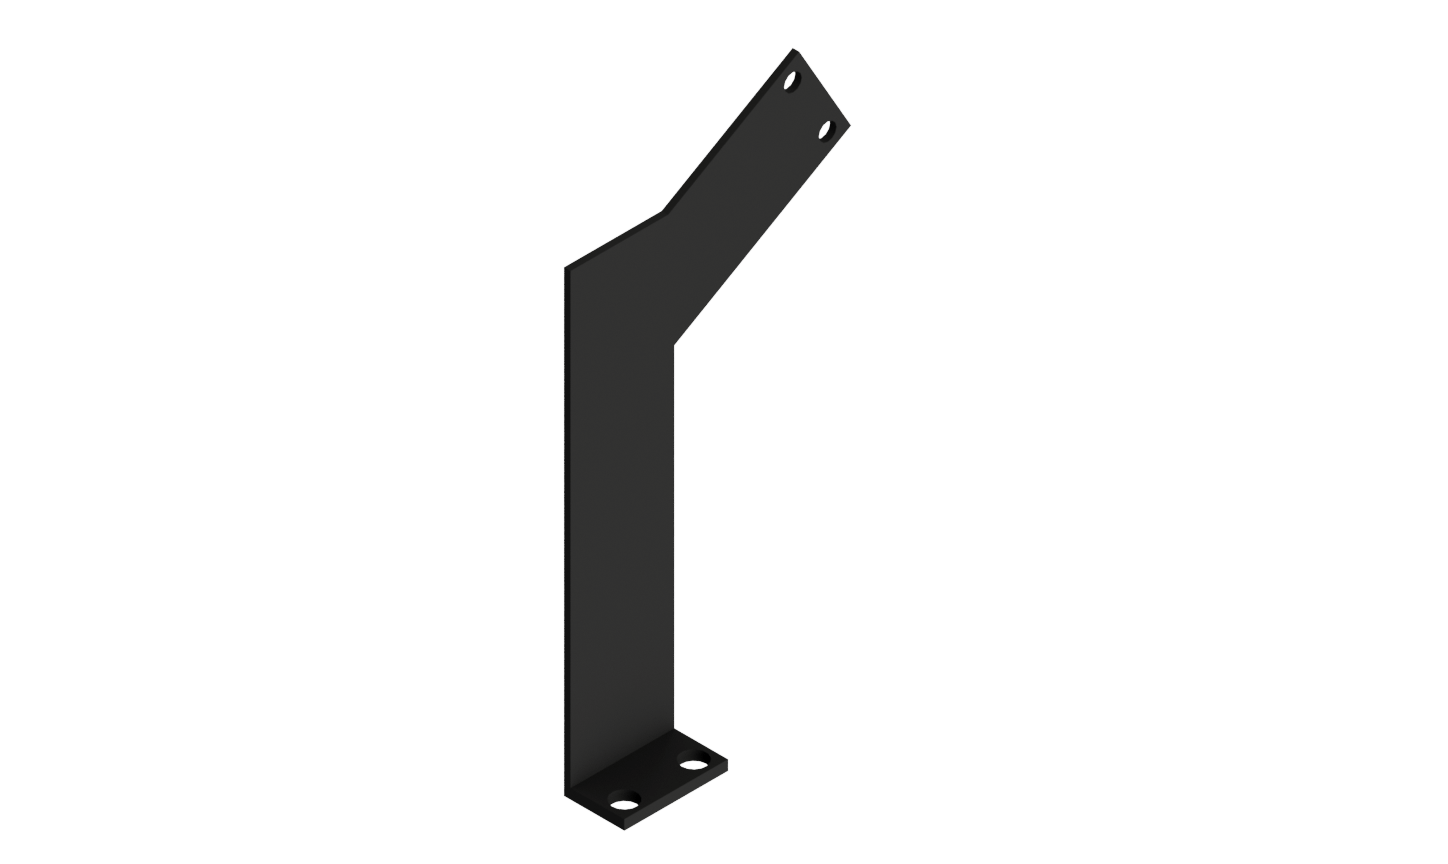
\includegraphics[width=8 cm]{fig/mech/AufhaengerIUnten}
    \caption{Aufhänger Unten}
    \label{fig:Aufhänger Unten}
\end{wrapfigure}

Das zweite Modul, welches in \autoref{fig:Aufhänger Unten} zu sehen ist, befindet sich nach dem Lagerrad und wird vom unteren Aufhänger in Position gehalten.
Der untere Aufhänger wird mit zwei Schrauben mit der Grundplatte des Gehäuses verschraubt.
Durch die dünne Bauweise und die Höhe des Aufhängers führt dies zu einer Instabilität des Moduls und des Aufhängers in Querrichtung, dieses Problem ist jedoch irrelevant, da es
zu keiner Krafteinwirkung auf dieser Achse kommt.
Um das Problem dennoch zu beheben, kann die Breite des Aufhängers variiert werden oder eine Querstrebe bei der Konstruktion hinzugefügt werden, da somit der Materialaufwand beim 3D-Drucken gering bleibt.\\
Der Aufhänger wird wie der andere Aufhänger über jeweils 2 Schrauben mit dem Kartenhalterungsmodul verschraubt.


\subsubsection{Kartenführung}
Um das Einführen der Karten zu erleichtern besitzen die Module Kartenführungen.

\textbf{Kartenführung Modul 1 oben:}

\begin{wrapfigure}{r}{8 cm}
    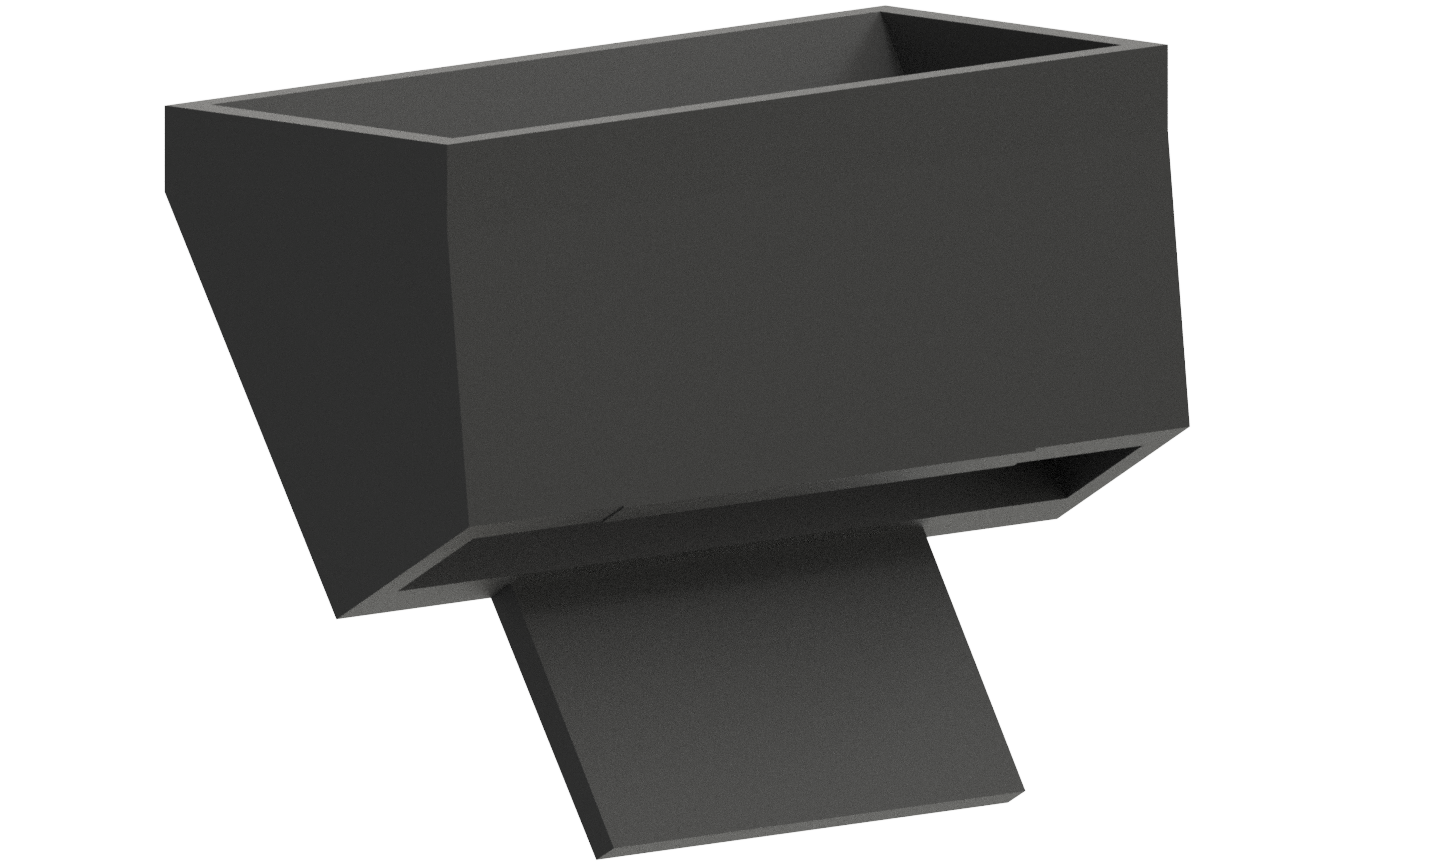
\includegraphics[width=8 cm]{fig/mech/KarteneinlaufNeu}
    \caption{Kartenführung Modul 1 oben}
    \label{fig:Kartenführung Modul 1 oben}
\end{wrapfigure}
Das erste Modul besitzt eine Kartenführung, siehe \autoref{fig:Kartenführung Modul 1 oben}, welche wie ein Trichter fungiert , der die Karten in die richtige Position bringt.
Die Kartenführung wird nicht mit dem Kartenhalterungsmodul verschraubt, sondern mit diesem verklebt.
Bei dieser Verbindung kann ohne Probleme eine Klebverbindung angewendet werden, da keine großen Kräfte auftreten.
Außerdem ist sie platzsparender und einfacher zu realisieren.
Die Berechnungen zu den Klebestellen findet man unter \autoref{subsubsec:KlebMod1}.

\pagebreak
\textbf{Kartenführung Modul 2 oben:}

\begin{wrapfigure}{r}{7 cm}
    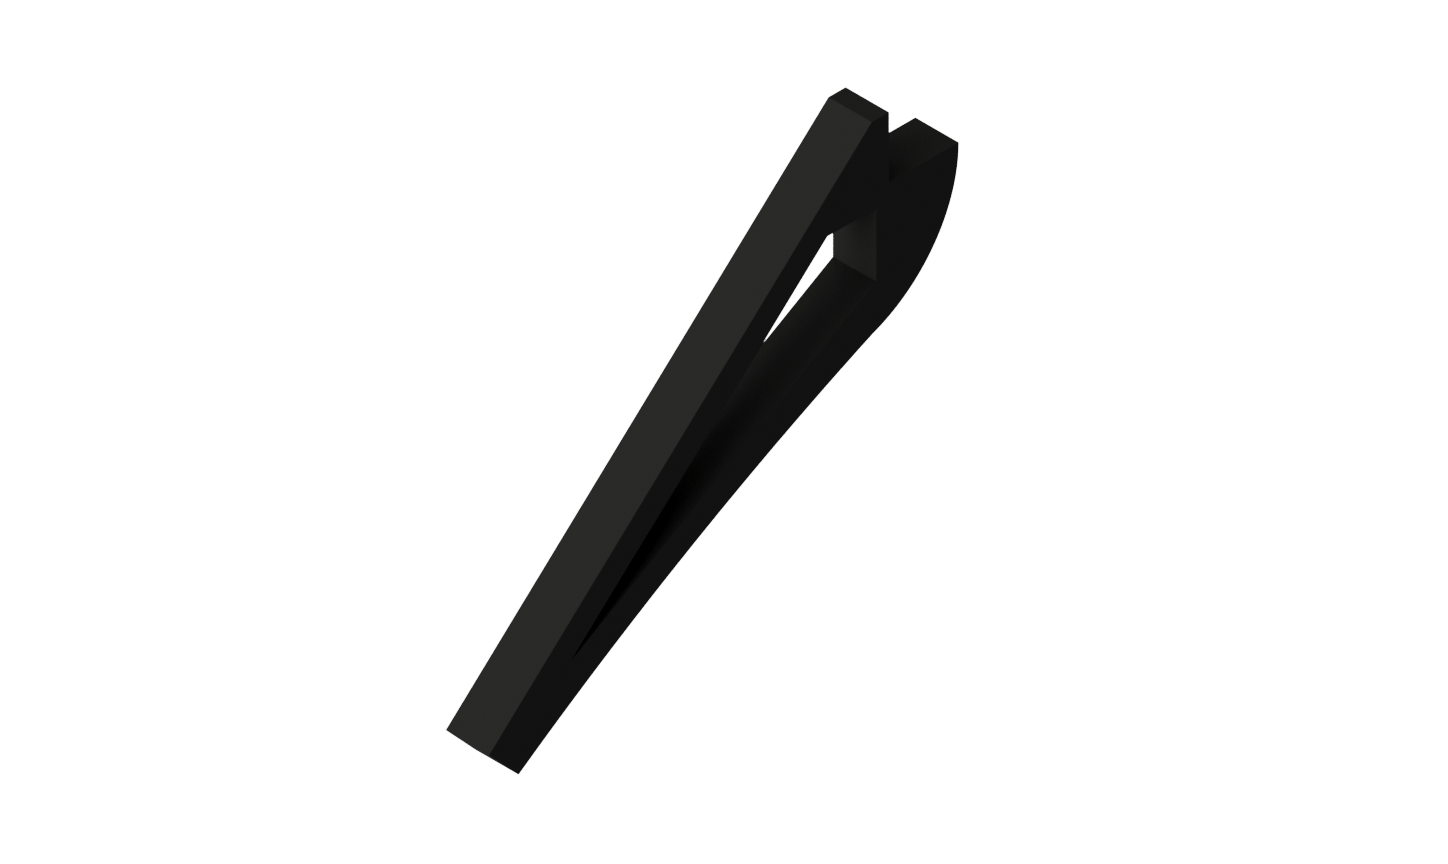
\includegraphics[width=7 cm]{fig/mech/StopperOben}
    \caption{Kartenführung Modul 2 oben}
    \label{fig:Kartenführung Modul 2 oben}
\end{wrapfigure}
Diese Kartenführung, siehe \autoref{fig:Kartenführung Modul 2 oben}, sorgt dafür, dass die Karten, welche aus dem Lagerrad geworfen werden, nicht zu früh herausfallen,
sondern erst über der Öffnung des Kartenhalterungsmodul.
Sie sind so entworfen, dass die Krümmung der Führungsfläche einen leicht größeren Radius besitzt wie der Maximalradius des Lagerrades.
Die zwei Kartenführungen sind mittels Klebeverbindungen an das Kartenhalterungsmodul befestigt, da keine großen Kräfte diese Bauteile angreifen.
Die Berechnungen dieser Klebestellen findet man unter \autoref{subsubsec:KlebMod2}. \\



\textbf{Kartenführung Modul 2 unten:}

\begin{figure}[H]
    \centering
    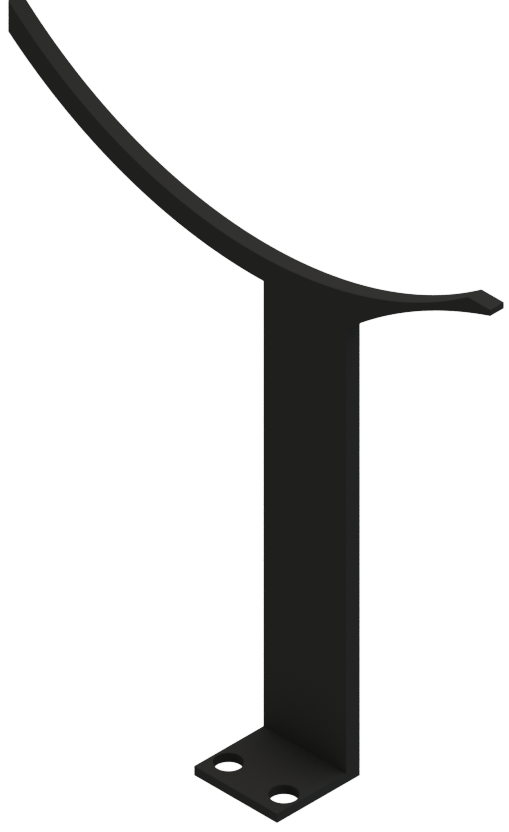
\includegraphics[width=6 cm]{fig/mech/FuehrungPLAUntenRechts}
    \caption{Kartenführung Modul 2 unten}
    \label{fig:Kartenführung Modul 2 unten}
\end{figure}

Die untere Kartenführung, die in \autoref{fig:Kartenführung Modul 2 unten} zu sehen ist, sorgt dafür, dass Karten, die nicht rechtzeitig aus dem Lagerrad fallen, nicht auf dem Boden der Maschine gelangen,
sondern durch die Kartenführung weiter im Lagerrad bleiben.
Diese Führung wird durch ihre Größe und Position nicht an dem Modul befestigt, sondern wird über jeweils zwei Schrauben mit dem Gehäuse
verbunden.
Durch die lange Bauform und die geringe Wandstärke des Bauteils, sollten Querstreben in die Konstruktion eingeplant werden,
da die Kartenführungen sich sonst bei leichtem Berührungskontakt schon stark bewegen.

\pagebreak
\subsection{Konstruktion der Kartenentnahme}
\begin{figure}[H]
    \centering
    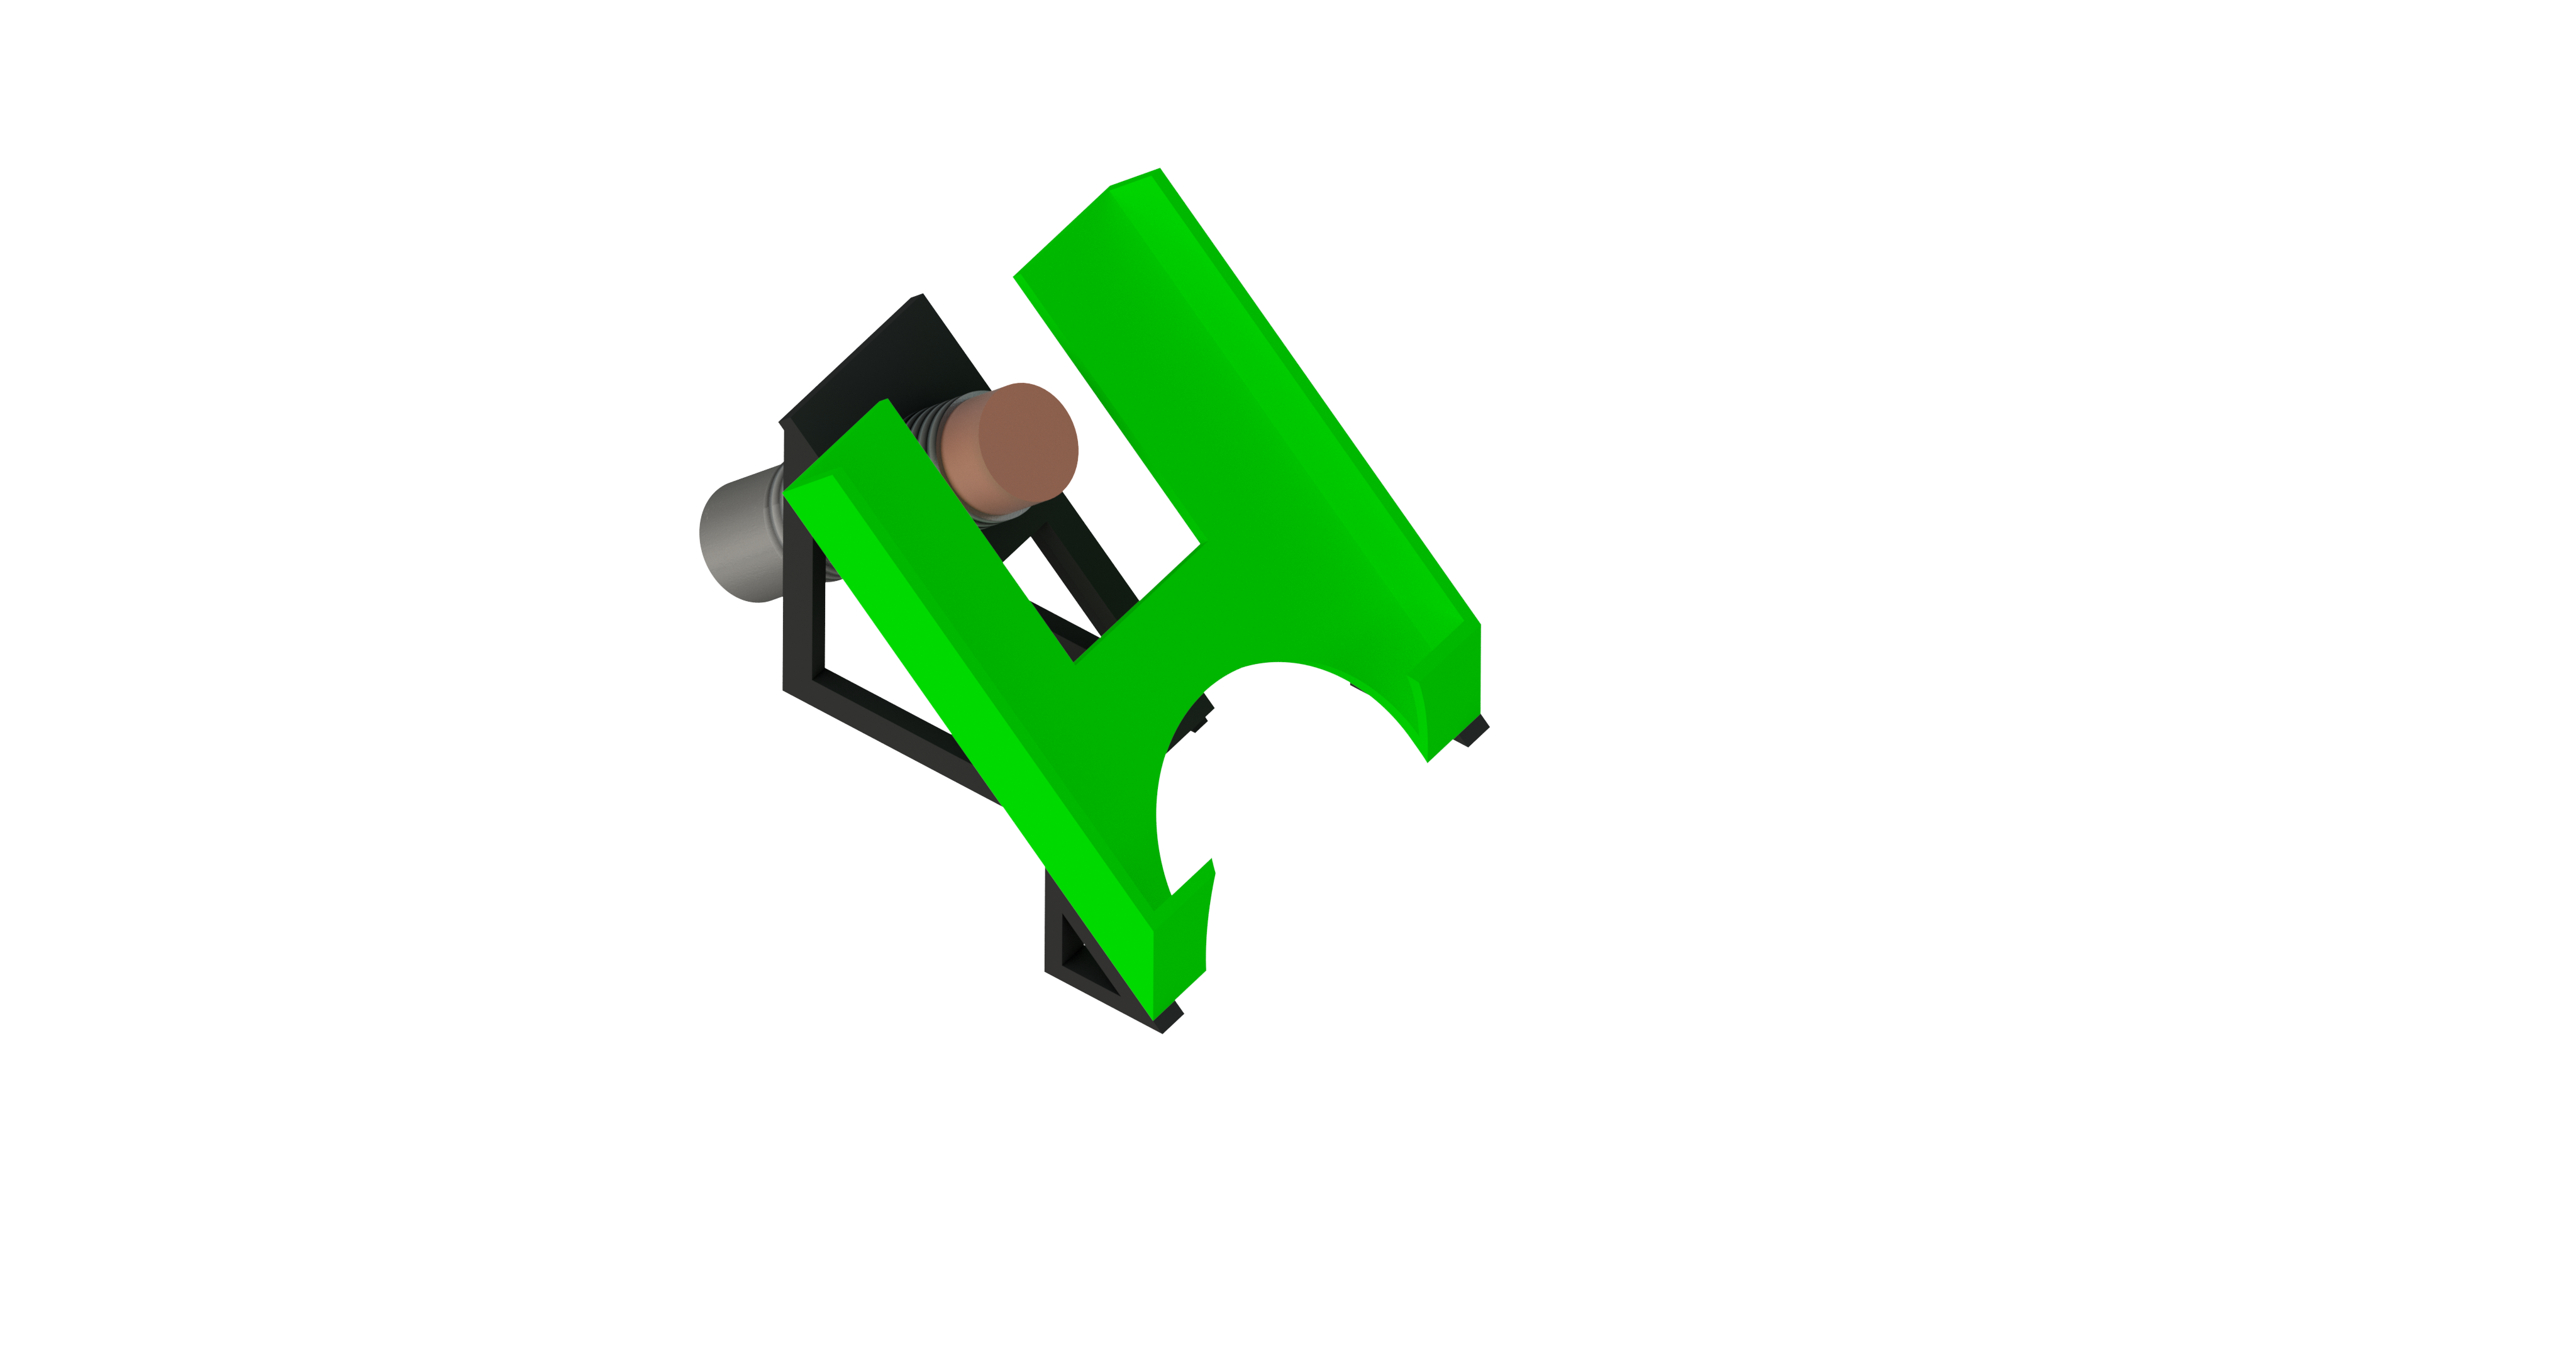
\includegraphics[width = 6cm]{fig/mech/AusgabeKomlett}
    \caption{Entnahmeplatte}
    \label{fig:GKartenentGes}
\end{figure}
Die Kartenentnahme, die in \autoref{fig:GKartenentGes} zu erkennen ist, befindet sich am unteren Ende der Maschine. Sie dient dazu, die Karten zwischenzulagern, bis der Spieler
sie entnimmt. Sie besteht aus folgenden Einzelbauteilen:\\

\begin{wrapfigure}{r}{6 cm}
    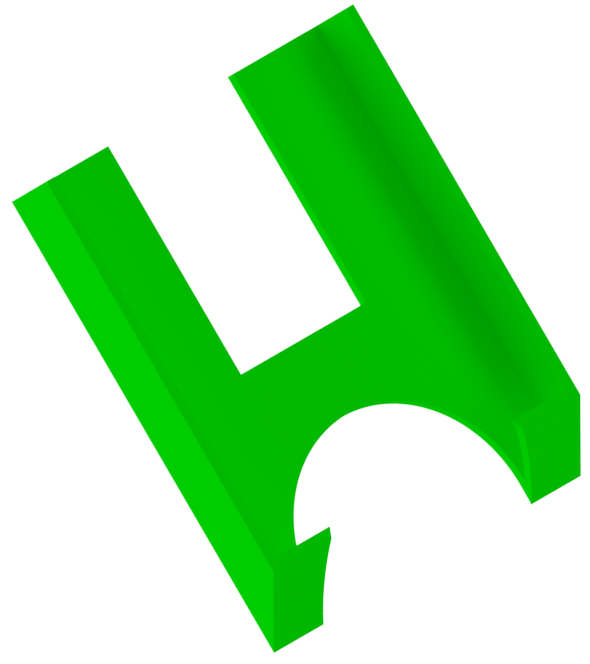
\includegraphics[width = 6cm]{fig/mech/Ausgabefach.png}
    \caption{Entnahmeplatte}
    \label{fig:Entnehmeplatte}
\end{wrapfigure}
\subsubsection{Entnehmplatte}

Dies ist das Grundbauteil, siehe \autoref{fig:Entnehmeplatte}, dieses Moduls.
Es fängt die Karten, welche vom Kartenhalterungsmodul ausgeworfen werden und lagert diese, bis
der Spieler diese manuell entnimmt. D
as Bauteil liegt in einem 45° Winkel und besitzt einen halbkreisförmigen Ausschnitt
an der Unterseite, welcher dazu dient, das Entnehmen der Karten zu vereinfachen.
Die rechteckige Ausnehmung in der Mitte des
Bauteils dient als Ausschnitt für den Sensor, sodass dieser überprüfen kann, ob sich Karten in dem Bauteil befinden.


\subsubsection{Sensorhalterung}

Da bei der Kartenentnahme auch geprüft wird, ob noch Karten in der Entnehmplatte liegen, wird eine Halterung für den
Sensor benötigt.
Dieses Bauteil, siehe \autoref{fig:Sensorhalterung2}, besitzt eine Bohrung, in welcher der Sensor durchgeführt wird und danach über zwei Muttern und
zwei Sicherungsringen befestigt wird.
Die rechteckige Ausfräsung auf der unteren Seite der Sensorhalterung dient lediglich für optische Zwecke und zur Materialverbrauchsminderung.

\begin{figure}[H]
    \centering
    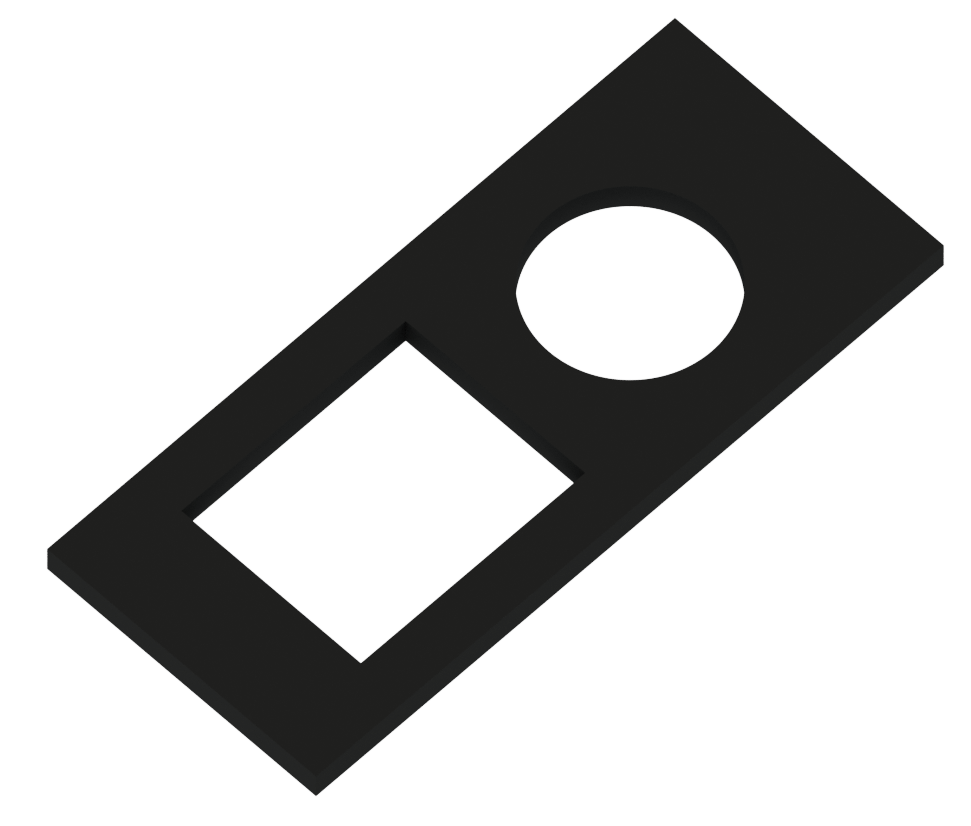
\includegraphics[width=8 cm]{fig/mech/SensorStuetze.png}
    \caption{Sensorhalterung}
    \label{fig:Sensorhalterung2}
\end{figure}

\subsubsection{Befestigungswinkel}


Da die Entnahmeplatte in einem 45° Winkel zum Gehäuse montiert werden muss, wurden dafür einfache Winkel, die in \autoref{fig:Befestigungswinkel} zu sehen sind, konstruiert und gefertigt.
Diese werden auf der einen Seite mit der Unterseite des Gehäuses verklebt, auf der anderen Seite mit der Entnehmplatte.
Auch hier können wieder Klebeverbindungen genutzt werden, da keine großen Kräfte auf die Bauteile angreifen.

\begin{figure} [H]
    \centering
    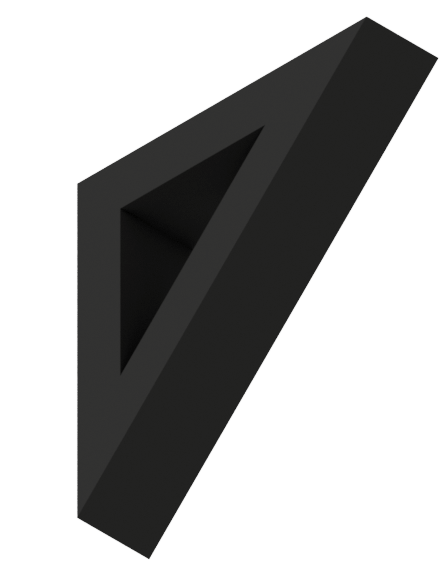
\includegraphics[width=4 cm]{fig/mech/Winkel}
    \caption{Befestigungswinkel}
    \label{fig:Befestigungswinkel}
\end{figure}

\subsubsection{Sensorhalterungswinkel}


Die beiden Sensorhalterungswinkel, die in \autoref{fig:Sensorhalterungswinkel} zu sehen sind, ermöglichen das Fixieren der Sensorhalterung in einem Winkel von 45°, parallel zur
Entnehmplatte.
Sie werden jeweils mit der Unterseite des Gehäuses und mit der Sensorhalterung verklebt.

\begin{figure}[H]
    \centering
    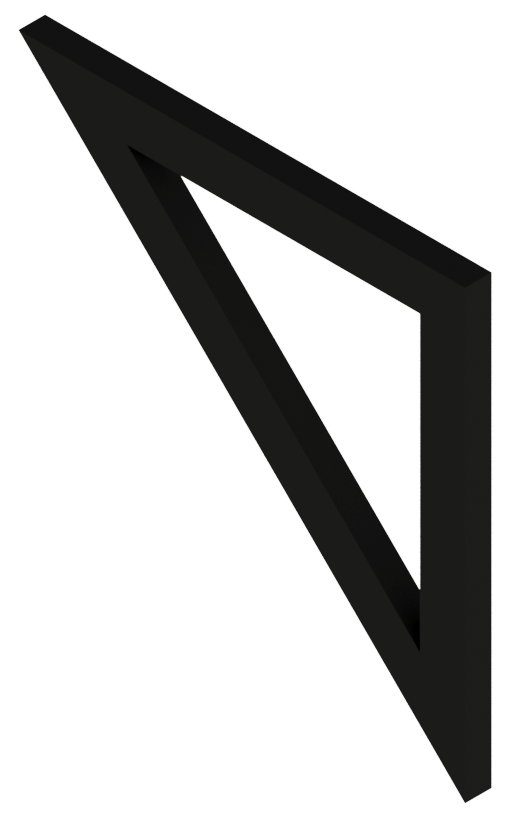
\includegraphics[width=4 cm]{fig/mech/WinkelSensor}
    \caption{Sensorhalterungswinkel}
    \label{fig:Sensorhalterungswinkel}
\end{figure}

\subsection{Konstruktion der Endschalterhalterung}
Dieses Bauteil, das in \autoref{fig:Enschalterhalterung} zu sehen ist, hat die Funktion, den Endschalter, der als Referenzpunkt für den Motor und das darauf montierte
Lagerrad gilt, zu befestigen.
Es besitzt zwei diagonale Bohrungen, über die der Endschalter verschraubt wird.
Die Endschalterhalterung wird auf der Rückseite über zwei Bohrungen mit dem Polycarbonatgehäuse verschraubt.
Das Bauteil muss so stabil gebaut sein, dass es einen leichten Zusammenstoß mit dem Lagerrad aushält, falls dieses
den Referenzpunkt anfährt.

\subsubsection{Enschalterhalterung}
\begin{figure}[H]
    \centering
    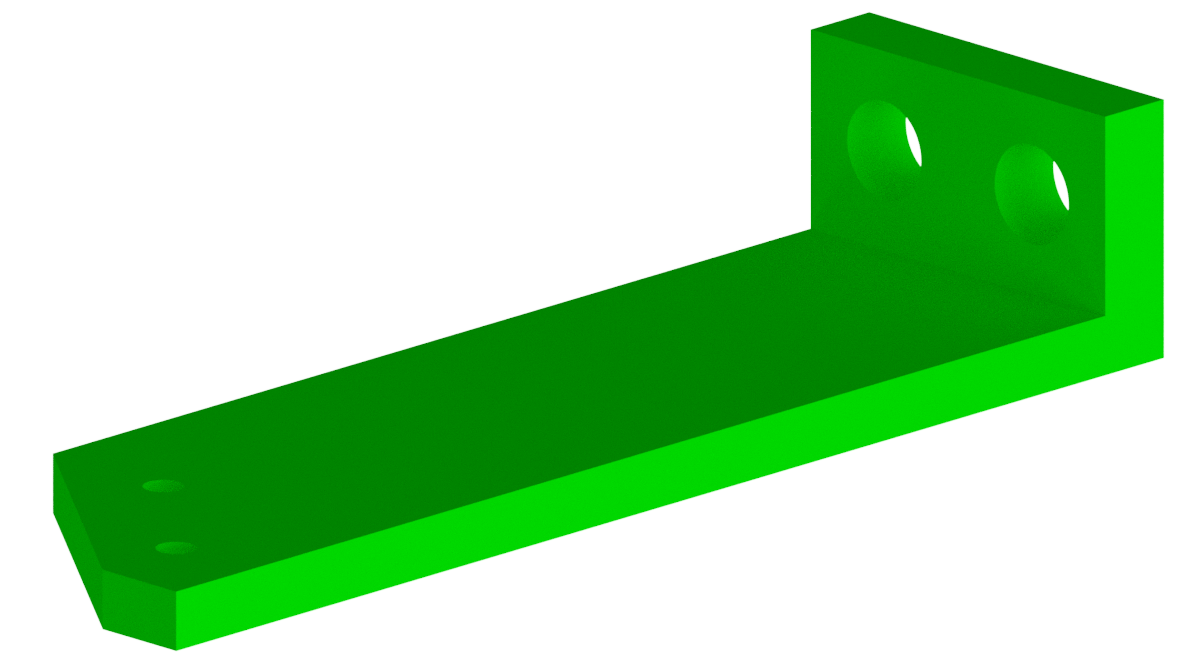
\includegraphics[width=8 cm]{fig/mech/AufhaengungEndschalter.png}
    \caption{Sensorhalterungswinkel}
    \label{fig:Enschalterhalterung}
\end{figure}

\subsection{Konstruktion des Gehäuses}
\footfullcite[Vgl.][]{fibox.ch2020}Das Gehäuse soll bei dieser Maschine optisch ansprechen und so klein wie möglich gehalten werden.
Für die Auswahl des Gehäusematerials kamen diverse Materialien in Frage:

\begin{table}[H]
    \centering
    \scalebox{0.8}{
    \begin{tabular}{|c|c|c|}
        \hline
        & \textbf{Vorteile}                                                                                                                                  & \textbf{Nachteile}                                                                                    \\ \hline
        \textbf{POLYCARBONAT (PC)}                    & \begin{tabular}[c]{@{}c@{}}Sehr hohe Schlagfestigkeit\\ Transparent\\ Leicht zu bearbeiten\\ Geringes Gewicht\\ Gute UV-Beständigkeit\end{tabular} & Vergleichsweise teurer                                                                                \\ \hline
        \textbf{ACRYLNITRIL-BUTADIEN-STYROL (ABS)}    & \begin{tabular}[c]{@{}c@{}}Geringes Gewicht\\ Günstiger als PC\end{tabular}                                                                        & \begin{tabular}[c]{@{}c@{}}Nicht für die Verwendung im Freien\\ nicht transparent\end{tabular}        \\ \hline
        \textbf{GLASFASERVERSTÄRKTES POLYESTER (GRP)} & \begin{tabular}[c]{@{}c@{}}Wetterbeständig\\ Stabil\\ Schlagfestig\end{tabular}                                                                    & \begin{tabular}[c]{@{}c@{}}Teurer als PC\\ schwer zu bearbeiten\\ beträchtliches Gewicht\end{tabular} \\ \hline
    \end{tabular}}
    \caption{Vergleich der Gehäusematerialien}
\end{table}

Da wir unser Material bearbeiten müssen, es portabel gestalten wollen und kein großes Budget haben, können wir
GRP als Gehäusematerial ausschließen.
Unser Gehäuse sollte auch optisch ansprechend sein und den Innenaufbau unserer
Maschine zeigen, somit ist ABS auch ausgeschlossen, da es nicht transparent ist.
Somit entschieden wir uns für
Polycarbonat als finales Gehäusematerial.

\subsubsection{Grundplatte}
Die Grundplatte ist die einzige Platte des Gehäuses, die nicht aus Polycarbonat besteht, sondern aus einem 12 mm dicken
Acrylglas.
Da uns dieses kostenlos zur Verfügung stand.\\
Um den unteren Aufhänger des Kartenhalterungsmoduls und die Kartenführung-Modul-2-Unten zu befestigen, befinden sich acht
Bohrungen in der Mitte der Grundplatte.
Diese Bohrungen sind mit einer Boden-seitigen Senkung versehen.
Somit kann die Senkkopfschraube ganz in die Grundplatte gesenkt werden und behindert nicht die Stabilität der Maschine.
Des Weiteren befindet sich in jeder Ecke eine weitere Bohrung mit Boden-seitiger Senkung.
Über diese Bohrung werden die Winkel verschraubt, welche die Grundplatte mit den restlichen Platten des Gehäuses verbindet.

\subsubsection{Seitenplatte Motor}
Diese Gehäuseplatte besitzt, genauso wie die Grundplatte, 4 Bohrungen an den Ecken der Platte, um sie über Winkel
mit den anderen Platten zu verbinden.
Weiters hat sie 4 Bohrungen im mittleren Bereich.
Über diese Bohrungen wird der Winkel der Motorhalterungsgruppe verschraubt.
Darüber hinaus besitzt sie eine innenseitige Einfräsung in der sich
zwei weitere Bohrungen befinden.
Diese Bohrungen werden für den Netzteilstecker sowie für den Taster benötigt.
Die Einfräsung ist notwendig, da diese beiden Bauteile ein Gewinde besitzen, über die sie mit dem Gehäuse verbunden werden.
Jedoch ist das Gewinde zu kurz für die dicke des Polycarbonats.

\subsubsection{Seitenplatte Lager}
Da diese Platte die Vorderseite des Gehäuses ist, befindetsich auf ihr auch das Liquid-Crystal-Display.
Um diesen zu montieren, hat die Platte eine rechteckige Ausfräsung im oberen Mittelbereich.
Seitlich, ober und unter der Ausfräsung, befinden sich je Seite zwei Langlöcher, über welche das Display mit dem Gehäuse verschraubt wird.
Unter dem Display besitzt diese Platte zusätzlich zwei Senklochbohrungen, über diese das Flanschlager verschraubt wird.
Zuletzt besitzt diese Platte auch vier Bohrungen an den Ecken, über die sie mit den anderen Platten verschraubt wird.

\subsubsection{Frontplatte}
Wie die vorherigen Platten, wird auch diese Platte über vier Bohrungen mit den Winkeln verschraubt.
Ansonsten hat diese Platte des Gehäuses nur zwei weitere Bohrungen, über welche die Endschalterhalterung verschraubt wird.

\subsubsection{Ausgabenplatte}
Da über diese Platte die Karten entnommen werden, besitzt die Ausgabenplatte eine rechteckige Einfräsung auf der unteren
Seite.
Weiters besitzt sie, wie die anderen Platten, vier Bohrungen an den Ecken.

\subsubsection{Topplatte}
Die Topplatte des Gehäuses hat eine rechteckige Einfräsung in der die Kartenführung-Modul-1-Oben
gesteckt wird.
Nach der Einfräsung besitzt diese Platte noch vier Bohrungen, über die der Aufhänger des Kartenhalterungsmodul
befestigt wird.
Wie auch bei allen anderen Platten, besitzt diese Platte auch vier Bohrungen an ihren Eckpunkten.

\begin{figure}[H]
    \centering
    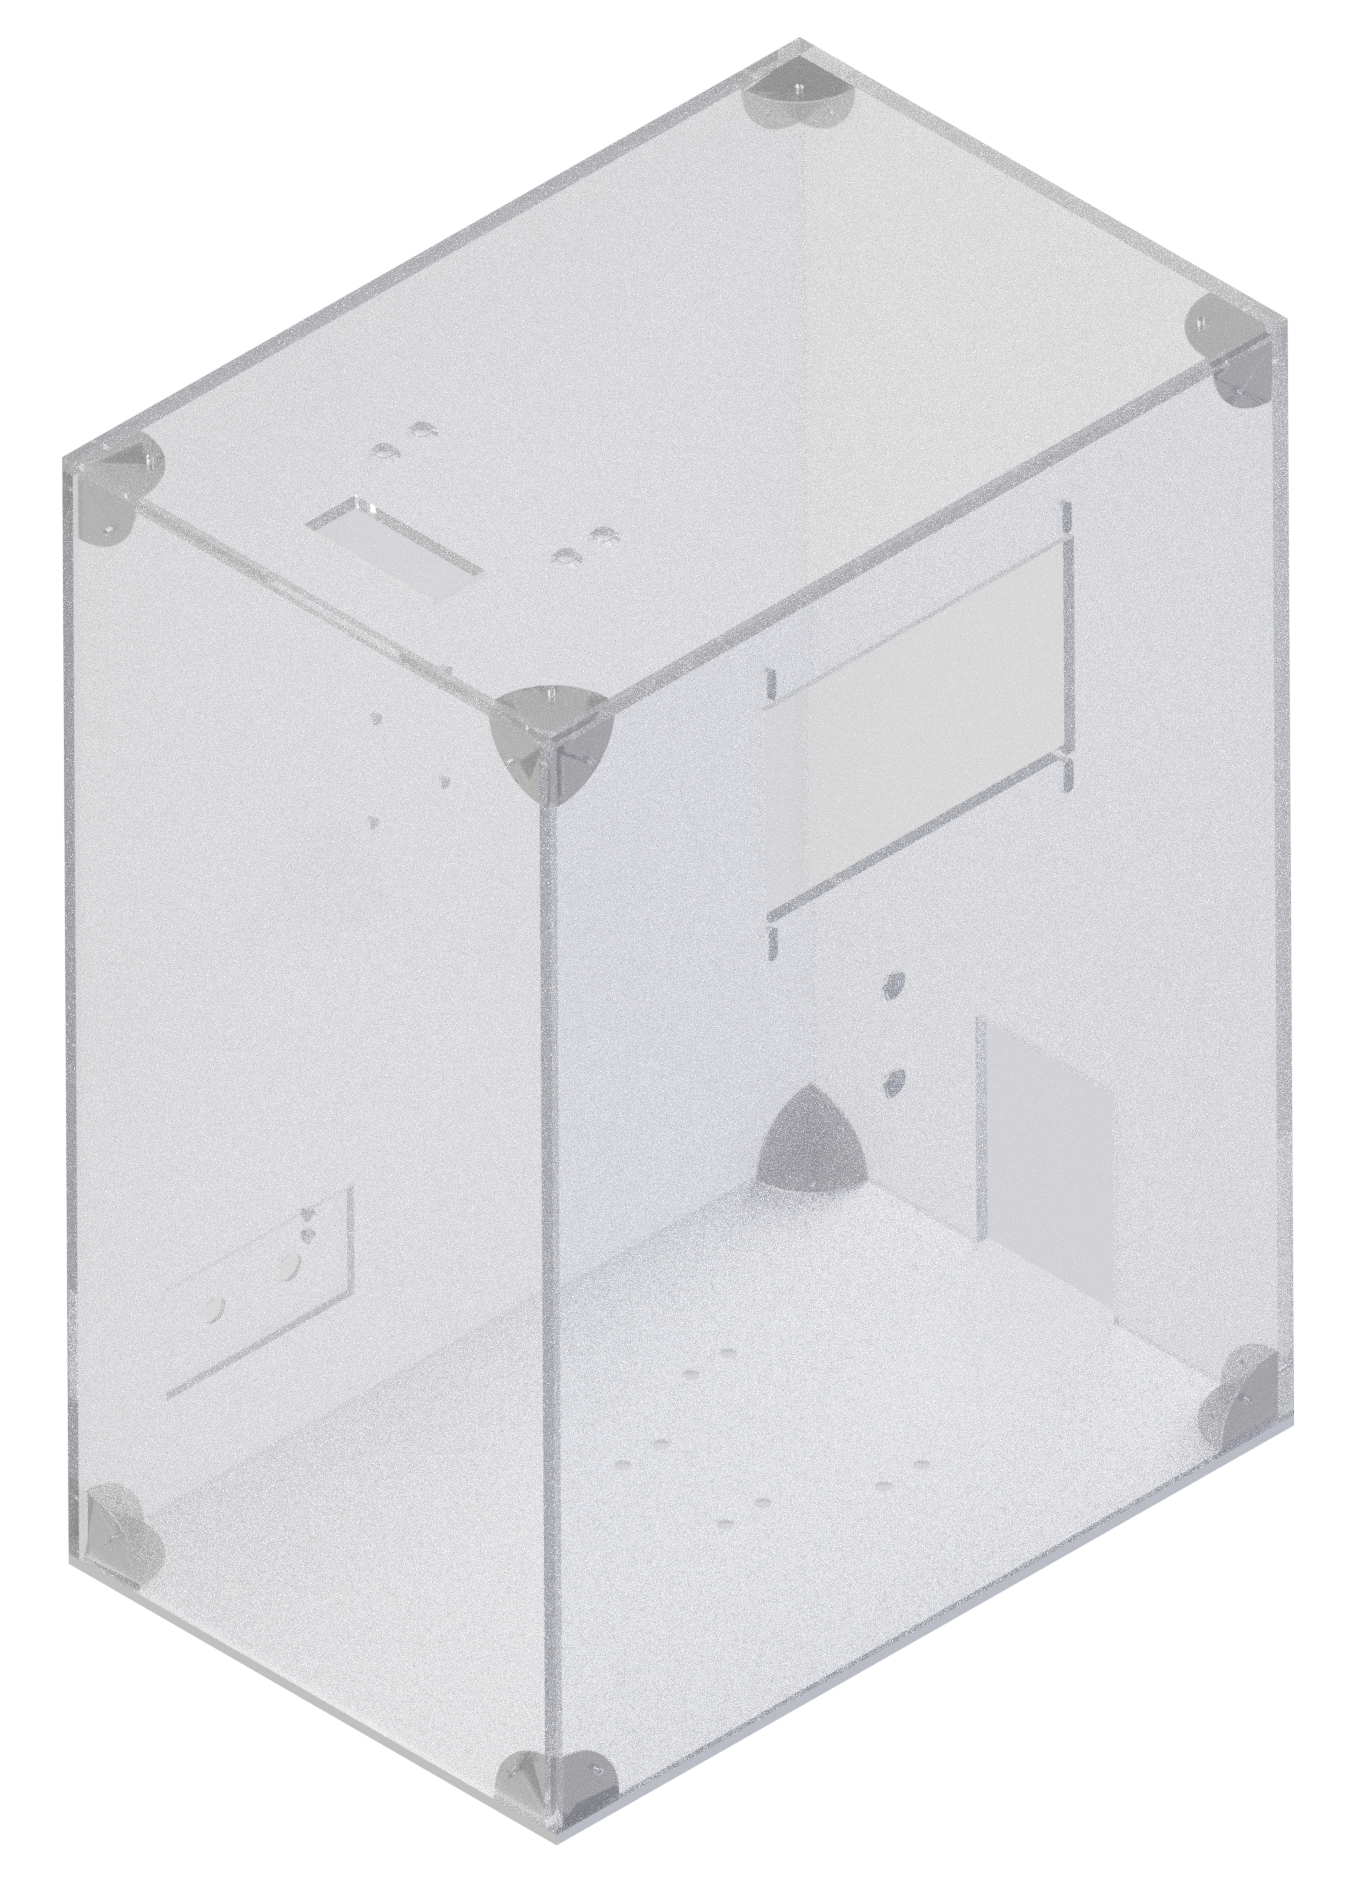
\includegraphics[scale=0.2,page=1]{fig/mech/Gehauuse.png}
    \caption{Gehäuse}
\end{figure}

\section{Berechnungen und Dimensionierungen}
\subsection{Auswahl des Motors}

Der Motor besitzt die Aufgabe, das Lagerrad zu drehen, daher muss der Motor so ausgelegt werden, dass
er das Lagerrad drehen und dessen Drehrichtung impulsartig wechseln kann.
Das Gewicht und die Trägheit des Lagerrades wird im leeren Zustand angenommen.
Zwar könnten sich bis zu 20 Karten in dem Lagerrad befinden,
jedoch ist das Gewicht, dass diese Karten erzeugen und die dazukommende Trägheit im Vergleich zum Lagerrad
so gering, das sie vernachlässigt werden kann.

\subsubsection{Bestimmung des Trägheitsmoment}

Als erstes muss das Trägheitsmoment bestimmt werden.
Dies kann über zwei Möglichkeiten erfolgen:
\begin{enumerate}
    \item Berechnung
    \item Analyse durch Inventor
\end{enumerate}

Es wurde die zweite Methode Analyse durch Inventor gewählt.
Zwar könnte das Trägheitsmoment händisch ausgerechnet werden,
dazu müsste man jedoch durch die komplexität des Bauteils alle Einzelteile extra berechnen und diese danach zusammenfügen.
Dies wäre zeitaufwändig und fehlerbehaftet.
Aus diesem Grund entschieden wir uns gegen diese Methode. \\

Um das Trägheitsmoment um den Schwerpunkt herauszufinden müssen in inventor folgende Schritte
angewandt werden.\\
Öffnen der Datei - Rechtsklick auf der Datei im Modellfenster(\autoref{fig:Modellleiste}) - iProberties öffnen - Physikalisch -  Schwerpunkt.\\
\begin{figure}[H]
    \centering
    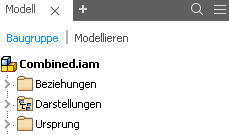
\includegraphics[scale=1,page=1]{fig/mech/Modellfenser}
    \caption{Modellfenster}
    \label{fig:Modellleiste}
\end{figure}


In \autoref{fig:iProperties} befinden sich alle Trägheitsmomente um den Schwerpunkt, der konkret gesuchte Schwerpunkt in unserem Beispiel ist
der um die Iyy Achse.

\begin{figure}[H]
    \centering
    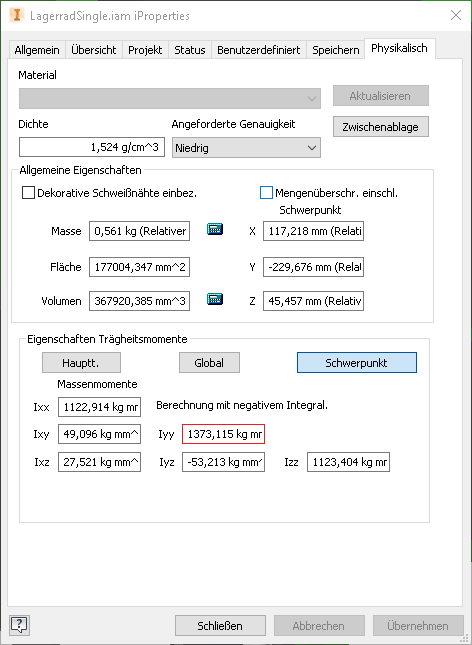
\includegraphics[scale=1,page=1]{fig/mech/iProberties.png}
    \caption{iProperties}
    \label{fig:iProperties}
\end{figure}

\textbf{Satz von Steiner:}\\
\footfullcite[Vgl.][]{Maschinenbau-Wissen.de2009a}Im nächsten Schritt muss das Trägheitsmoment vom Schwerpunkt auf die tatsächliche Drehachse verschoben werden.
Dazu wird der Satz von Steiner benötigt:\\
\begin{align*}
    J_{2} &= J_{1}+m\cdot d^{2} \\
    J_{2} &= 1373,115 kgmm^{2}+0,561kg\cdot \sqrt{45,493^{2}mm^{2}+45,493^{2}mm^{2}}^{2} \\
    J_{2} &= 1373,115 kgmm^{2}+0,561kg\cdot 64,3368mm^{2} \\
    J_{2} &= 3695,2208 kgmm^{2} \\
\end{align*}

Als nächstes wird die Formel für die Summe aller Momente aufgestellt:
\begin{align*}
    \sum M &= 0 = -M_{motor}+ J\cdot \alpha\\
\end{align*}

\footfullcite[Vgl.][]{Grund-Wissen.de2018}Um die Winkelbeschleunigung $\alpha$ zu berechnen, wird die Winkelgeschwindigkeit $\omega$ benötigt.

\begin{align*}
    \omega &= 2 \cdot \pi \cdot\\
    \omega &= 2 \cdot \pi \cdot 0,5 Hz\\
    \omega &= \pi \tfrac{rad}{s}\\
\end{align*}

Nun kann über die Winkelgeschwindigkeit und über die Zeit die Winkelbeschleunigung berechnet werden.

\begin{align*}
    \alpha &= \frac{\Delta \omega }{\Delta t}\\
    \alpha &= \frac{\pi }{0,25} \tfrac{rad}{s^{2}}\\
\end{align*}

Setzt man nun die Winkelbeschleunigung in die Formel der Summe aller Momente ein, bekommt man das notwendige
Haltemoment des Motors.
\begin{align*}
    M_{Motor} &= 0,003696kgm^{2} \cdot \frac{\pi }{0,25}\tfrac{rad}{s^{2}}\\
    M_{Motor} &= 0,046Nm\\
\end{align*}




\textbf{Eckdaten des gewählten Motors}
\begin{itemize}
    \item Motortyp: Bipolarer Schrittmotor
    \item Schrittwinkel: 1,8 Grad
    \item Haltemoment: 0,59 Nm
    \item Bemessungsstrom / Phase: 2,0 A
    \item Gewicht: 380 g
    \item Rahmengröße 41 mm x 41 mm
\end{itemize}
\subsection{Auswahl der Vakuumaktorik}
\subsubsection{Auswahl der Vakuumpumpe}
Um die Vakuumpumpe auszuwählen, muss zuerst die erforderliche Druckdifferenz berechnet werden.
Da die Karten liegend angehoben werden, kommt für die Berechnung der theoretischen Haltekraft der typische Lastfall 1
zum Einsatz.
Zwar wird dieser für eine vertikale Kraftrichtung eingesetzt, und nicht wie bei dem Beispiel in einem
60° Winkel, dennoch ist er der Lastfall, der unserem Beispiel am nächsten kommt.
\footfullcite[Vgl.][]{schmalz.com2020}Die theoretische Haltekraft wird mit folgender Formel berechnet:
\begin{align*}
    F_{TH} &= m \cdot (g + a) \cdot S
\end{align*}

F\textsubscript{TH}.... theoretische Haltekraft [N] \\
m.... Masse [kg]\\
g.... Erdbeschleunigung [9,81 m/s²]\\
a.... Beschleunigung der Anlage [m/s²]\\
S.... Sicherheitsfaktor \\

Die Masse einer standardmäßigen  Spielkarte liegt bei 2 Gramm, darum wird mit einem Wert von m = 2g gerechnet.
Die maximale Wegbeschleunigung des Saugnapfes wird beim Einziehen des Hubmagnetes erreicht und
beträgt 1,8m/s²,
daher wird für die Beschleunigung a = 1,8m/s² eingesetzt.
Da ein geringer Unterdruck zur nächsten Karte herrscht, wird eine Sicherheit von 20 gewählt.
Setzt man die Werte in die Formel ein, bekommt man folgendes Ergebnis: \\
\begin{align*}
F_{TH} &= 0,002kg\cdot (9,81\frac{m}{s^{2}}+1,8\frac{m}{s^{2}})\cdot 20\\
F_{TH} &= 0,4644N\\
\end{align*}
Um die Druckdifferenz zu berechnen, muss als erstes die Fläche des Saugers berechnet werden.
Mit einem Durchmesser des Saugers von 20mm ergibt sich eine Fläche von:
\begin{align*}
A &= r^{2}\cdot \pi\\
A &= 0,02m^{2}\cdot \pi\\
A &= 0,001257m^{2}\\
\end{align*}
Setzt man die Werte in die Formel ein, bekommt man folgende Druckdifferenz:
\begin{align*}
\triangle P &= \frac{F_{TH}}{A}\\
\triangle P &= \frac{0,4644N}{0,001257m^{2}}\\
\triangle P &= 369,4511Pa\\
\end{align*}
Da der berechnete Wert unbeachtlich klein ist, kann eine möglichst schwache Pumpe ausgewählt werden.
Diese beansprucht wenig Platz, braucht wenig Strom und ist leise.
Schlussendlich wurde eine Pumpe mit einer Leistung von 2,15W und einer Spannung von 5V DC ausgewählt.\\
\textbf{Daten der Pumpe}
\begin{itemize}
    \item Spannung 5V (max 6V)
    \item Druck: > 400 mmHg (> 53329 Pa)
    \item Verbrauch: 430 mA
    \item Lautstärke: 63 dB
    \item Durchflussrate: > 1,8 Liter pro Minute
\end{itemize}



\subsubsection{Auswahl des Ventils}
Da der Saugnapf nicht immer einen Unterdruck haben darf, wird eine Ventil benötigt.
Die beiden Voraussetzungen waren es, dass das Ventil einerseits mit einem niedrigen Spannungspegel betrieben werden kann.
Andererseits muss es dazu im Stande sein, zwei verschiedene Pneumatikleitungen zu schalten.\\
\textbf{Eckdaten des ausgewählten Ventils}
\begin{itemize}
    \item Nennspannung: DC 6V
    \item geeigneter Spannungsbereich:DC 5V - DC 6V
    \item Strom: 220 mA
    \item Leistung: <2W
    \item Druckbereich: 0-350 mmHg
\end{itemize}

\subsection{Berechnung der Klebeverbindungen}
Für die Klebeverbindungen verwenden wir einen 2-Komponenten-Epoxy-Kleber, welcher sich hervorragend für das
Kleben von harten Kunststoffen, wie gedrucktes PLA, eignet.

\subsubsection{Klebeverbindung Kartenhalterunsmodul 1} \label{subsubsec:KlebMod1}
\footfullcite[Vgl.][]{Wittel2013}Beim Kartenhalterunsmodul-Oben wird die Kartenführung-Modul-1-Oben mit dem Kartenhalterunsmodul 1 verklebt.
Die Formel zum Berechnen der Klebefläche lautet:
\[\sigma _{K} &= \frac{F}{A_{K}} = \frac{F}{b\cdot t}\leq \frac{\sigma _{KB}}{S}\]

$\sigma_{K}$.... Bindefestigkeit der Klebefläche \\
$\sigma_{KB}$.... Bindefestigkeit nach TB 5-2 und TB 5-3 (Maschinenelemente Tabellenbuch)\\
F.... Größte zu übertragende Kraft [N]\\
A\textsubscript{K}.... Klebefläche [mm²]\\
b.... Breite der Klebefläche [mm]\\
t.... Tiefe der Klebefläche [mm]\\
S.... Sicherheitsfaktor\\

Für die Kraft werden 50 N angenommen, dies entspricht in etwa der Gewichtskraft von 5,1kg
und simuliert somit ein kraftvolles Ankommen des Spielers an der Trichtervorrichtung.
Die Fläche der Klebefläche A\textsubscript{K} ergibt sich durch die Breite und der Tiefe der Klebefläche, wobei
die Breite der Klebefläche  40mm beträgt und dessen Länge 20mm.
Der Wert $\sigma_{K}$ ist aus der Tabelle 5-3 im Tabellenbuch \footfullcite[Vgl.][]{Wittel2013Tab} auszulesen.
Um die 3-Fache Sicherheit zu gewährleisten, wurde der Sicherheitsfaktor 3 gewählt.

\begin{align*}
\sigma _{K} &= \frac{50}{40\cdot 20}\leq \frac{21}{3}\\
\sigma _{K} &= 0,0625\leq 7\\
\end{align*}
Da die Gleichung sich als wahr erweist und die Klebefläche sichtlich überdimensioniert ist, lässt sich erschließen,
dass das Bauteil auch einen Zusammenstoß mit höherer Kraft überstehen, ohne dass sich die Klebeverbindung löst.

\subsubsection{Klebeverbindung Kartenhalterunsmodul 2} \label{subsubsec:KlebMod2}
Hierbei werden die Kartenführungen-Modul-2-Oben mit dem unteren Kartenhalterunsmodul verklebt.
Für die Berechnung der Klebefläche wird wieder folgende Formel benötigt.
\begin{align*}
\sigma _{K} &= \frac{F}{A_{K}} = \frac{F}{b\cdot t}\leq \frac{\sigma _{KB}}{S}\\
\end{align*}
$\sigma_{K}$.... Bindefestigkeit der Klebefläche \\
$\sigma_{KB}$.... Bindefestigkeit nach TB 5-2 und TB 5-3 (Maschinenelemente Tabellenbuch)\\
F.... Größte zu übertragende Kraft [N]\\
A\textsubscript{K}.... Klebefläche [mm²]\\
b.... Breite der Klebefläche [mm]\\
t.... Tiefe der Klebefläche [mm]\\
S.... Sicherheitsfaktor\\

Die Klebefläche schließt sich aus 2 Teilen zusammen, da das Bauteil zwei dieser Klebeflächen besitzt.
\begin{align*}
A_{K} &= b_{1}\cdot t_{1}+b_{2}\cdot t_{2}\\
A_{K} &=3 mm\cdot 5 mm+7 mm\cdot 5 mm\\
A_{K} &= 50 mm^{2}\\
\end{align*}
\footfullcite[Vgl.][]{Grund-Wissen.de2018}Die größte zu übertragende Kraft tritt dann ein, wenn der ganze Kartenstapel mit 20 Karten aus dem
Lagerrad und auf den Punkt mit der Größten Hebelkraft geworfen wird.
Somit müssen wir als erstes die Bahngeschwindigkeit des Lagerrades ausrechnen:
\begin{align*}
v &= \omega \cdot r\\
v &= 2 \cdot \pi \cdot f \cdot \cdot r\\
\end{align*}
v.... Bahngeschwindigkeit[m/s²]\\
$\omega$.... Winkelgeschwindigkeit[rad/s]\\
f.... Frequenz[1/T]\\
r.... Radius\\
\begin{align*}
v &= 2 \cdot \pi \cdot 0,5 Hz \cdot 0,127 m\\
v &= 0,39918 \tfrac{m}{s}\\
\end{align*}

Nun wird über die Geschwindigkeit die Beschleunigung ausgerechnet:
\begin{align*}
a &= \frac{v}{t}\\
\end{align*}
a.... Beschleunigung[m/s²]\\
v.... Bahngeschwindigkeit[m/s]\\
t.... Zeit[s]\\
\begin{align*}
a &= \frac{0,39918\tfrac{m}{s}}{0,25s}\\
a &= 1,59672\tfrac{m}{s^{2}}\\
\end{align*}
Anschließend wird über die Masse und über die Beschleunigung die Kraft der herausfallenden Karten ausgerechnet:
\begin{align*}
F &= m \cdot a
\end{align*}
F.... Kraft[N]\\
m.... Masse[Kg]\\
a.... Beschleunigung[m/s²]\\
\begin{align*}
F &= 0,04 kg \cdot 1,59672\tfrac{m}{s^{2}}\\
F &= 0,0638N\\
\end{align*}
Das Maximalmoment wird nun über die errechnete Kraft F und der maximalen Hebellänge l ausgerechnet.
\begin{align*}
M_{max} &= F\cdot l\\
M_{max} &= 0,06386N\cdot 55mm\\
M_{max} &= 3,4862\tfrac{N}{mm}\\
\end{align*}
F.... Kraft[N]\\
l.... Abstand[mm]\\

\begin{align*}
\sigma _{K} = {\frac{\frac{M_{max}}{2}}{50mm^{2}}} &\leq \frac{\sigma _{KB}}{S}\\
\sigma _{K}= \frac{\frac{3,4862\tfrac{N}{m}}{2}}{50m^{2}} &\leq  \frac{21 \tfrac{N}{mm^{2}}}{3}\\
\sigma _{K} = 0,034862 \tfrac{N}{mm^{2}} &\leq 7 \tfrac{N}{mm^{2}}\\
\end{align*}
Da die Gleichung sich als wahr erweist, halten die Führungen die Kraft der herausfallenden Karten
aus.
Durch die enorme Überdimensionierung ist zu erkennen, das auch eine größere Kraft
keine Probleme bereiten würde.

\newpage
\section{Fertigung der Bauteile}
\subsection{Werkstoffwahl}
\footfullcite[Vgl.][]{Maschinenbau-Wissen.de2009} \footfullcite[Vgl.][]{ Lernhelfer.de2020}Anfangs stellte sich die Frage, mit welchem Werkstoff die Prototypen sowie die fertigen Bauteile der
Maschine produziert werden sollen.
Da die Bauteile ein niedriges Gewicht haben sollen sowie billig und schnell produzierbar
sein sollten, wurde Kunststoff ausgewählt.
Es wurden folgende Arten zur Verarbeitung von Kunststoff in Betracht gezogen:
\subsubsection{Extrudieren}
Das geschmolzene Material wird beim Extrudieren über Düsen gepresst.
Über Ringförmige Düsen können Rohre entstehen, über Schlitzförmige können Platten entstehen, somit entspricht der Querschnitt der Düse immer auch den Querschnitt des erzeugten Profils.
Der Vorteil dabei ist, dass sogar Formen mit Hohlräumen an einem Tag herstellbar sind.
Die erzeugten Platten werden oftmals noch weiterverarbeitet, indem man sie erwärmt und über eine Form zieht, oder durch
Vakuum und Druck in die gewünschte Form bringt.
Es gibt noch diverse andere Arten von Extrudern, wie den Schneckenextruder.
Dieser lässt sich weiter unterteilen in den Einschnecken-, gegenlauf Doppelschnecken- und gleichläufige Doppelschneckenextruder.
Der Vorteil der Doppelschneckenextruder liegt dabei in ihrem guten Mischungsverhältnis, jedoch sind Einschneckenextruder um vieles günstiger.
Andere Bauformen des Extruders wären der Kolbenextruder sowie der Planetwalzenextruder.
Für Keramikmaterialien werden in der Regel Kolbenextruder eingesetz.
Um PVC-Folien Herzustellen werden am häufigsten Planetwalzenextruder benutzt.

\subsubsection{Spritzgießen}
Über das Spritzgießen können komplexe Bauteile mit einer hohen Qualität hergestellt werden.
Die Maschine besteht dabei aus einer sogenannten Spritzeinheit und einer Schließeinheit.
Die Spritzeinheit besteht aus einem Extruder mit einer beweglichen Schnecke, diese stößt die Polymerschmelze durch die Vorwärtsbewegung der Schnecke in das Werkzeug aus.
Um das Werkzeug zu öffnen und zu schließen und somit den Ausstoß des Polymeres zu ermöglichen wird die Schließeinheit
benötigt.
Bei Beginn des Spritzgusses wird eine rotierende Schnecke mit einem Granulat oder einem Pulver befüllt.
Das Material wird danach durch die rotierende Bewegung der Schnecke geschmolzen und nach vorne befördert.
Das geschmolzene Material staut sich an der Spitze, da das Werkzeug durch die Schließeinheit noch nicht geöffnet wurde und somit entsteht ein hoher Druck.
Da die Schnecke beweglich gelagert ist, dreht sich diese selbst aus dem verdichteten Polymere heraus.
Wird das Material dann eingespritzt, öffnet sich das Werkzeug und die Schnecke wird unter Druck gesetzt, sodass das
Material in die gewünschte Form gespritzt werden kann.
Beim Spritzgießen wird immer mehr Material mitgedruckt, da sich beim Abkühlen des Spritzgusses das Volumen leicht
verringert.
Da das Werkzeug des Spritzgusses sehr teuer ist, müssten einige tausend Stück unserer Bauteile hergestellt werden,
sodass sich der Spritzguss rentiert.

\subsubsection{Blasformen}
Bei dieser Form der Kunststoffverarbeitung wird Druckluft in ein Schlauchstück eingeblasen, das zuvor über ein Werkzeug
extrudiert wurde.
Über dieses Verfahren können somit Hohlkörper, wie Flaschen oder Kanister, hergestellt werden.
Über ringförmige Düsen können auch Folien hergestellt werden, dieses Verfahren wird dann auch als Folienblasen bezeichnet.

\subsubsection{Kalandrieren}
Beim Kalandrieren schmilzt man eine Kunststoffmasse zwischen zwei erwärmten, sich gegeneinander drehenden Walzen auf.
Weitere Walzen werden für die benötigte Dicke der Folie dazugeschaltet und sorgen gleichzeitig für die Homogenisierung.
Über das Kalandrieren werden Platten oder Folien hergestellt, man kann aber auch andere Materialien wie Metalle, Papier
oder Gummi verwenden.

\subsubsection{Rotationsformen}
Bei diesem Produktionsverfahren werden größere, hohle und nahtlose Kunststoffteile hergestellt.
Es befindet sich ein geschmolzenes Kunststoffgranulat in einer rotierenden Form, dieses Granulat setzt sich beim Auskühlen an den
Rand der rotierenden Form ab und erzeugt somit eine hohle Kunststoffform.
Der Vorteil hierbei liegt bei den niedrigeren Kosten, jedoch ist man nur in der Lage primitivere hohle Formen herzustellen.

\subsubsection{Verarbeitung von duroplastischer Kunststoffe}
Um duroplastische Kunststoffe zu verarbeiten, müssen sie mittels Synthese in die gewünschte Form gebracht werden, da sie
nicht wärmeformbar sind.
Dazu werden meist pulverförmige Vorprodukte direkt in eine Form gebracht, und nach Bedarf Farb- oder Zusatzstoffe beigefügt.
Danach werden sie unter Katalysator- und Wärmeeinfluss zum Endprodukt ausgehärtet.
Durch dieses Verfahren können auch metallische Werkstoffe mit Duroplasten verbunden werden, wie zum Beispiel
Glas-verstärkte Kunststoffe (GFK), die vielfältig in der Luft- und Wasserfahrt zum Einsatz kommen.

\subsubsection{Kleben}
Kleben ist ein Fügeverfahren von Kunststoffen, bei dem meist Duroplasten und Elastomere zusammengefügt werden.
Jedoch benötigt man dazu Kunststoffe mit polaren Eigenschaften, um eine erfolgreiche Klebeverbindung zu garantieren.
Um diese Eigenschaften zu erschaffen, müssen viele Kunststoffe mit Korona- oder Plasmabehandlung vorbereitet werden,
um die notwendige Benetzbarkeit aufzuweisen.\\
Physikalische Kleber können in drei Kategorien eingeteilt werden:
\begin{itemize}
    \item \textbf{Verdunstung}: Diese Kleber härten durch Verdunstung des Lösemittels aus.
    \item \textbf{chemische Kleber}: Aushärtung durch chemische Reaktion
    \item \textbf{molekulare Struktur}: Besitzen bereits vor dem Auftragen über eine molekulare Struktur
\end{itemize}

\subsubsection{Schweißen}
Schweißen ist das zweite Fügeverfahren für Kunststoff.
Bei diesem Verfahren muss das Material in erster Linie die Fähigkeit zum Schmelzen verfügen.
Da nur Thermoplaste diese Eigenschaft besitzen, ist es die einzige Kunststoffart, die sich gut zum Schweißen eignet.
Für das Erwärmen und Aufschmelzen des Materials können unterschiedliche Techniken angewendet werden:
\begin{itemize}
    \item Elektrische Induktionsheizung (Heizelementschweißen)
    \item Heiße Druckluft (Warmgasschweißen)
    \item Licht- oder Laserstrahlung (Strahlungsschweißen)
    \item Reibung (Reibungsschweißen)
\end{itemize}

\subsubsection{3D-Druck}
Der 3D-Druck ist kein Umformverfahren oder Fügeverfahren, sondern ein Urformverfahren mit dem man in kurzer Zeit präzise Kunststoffteile
drucken kann.
Da das 3D-Drucken billig, schnell und eine hohe Genauigkeit aufweist, nahmen wir es zum Bau unserer Prototypen.
Genaueres zum 3D-Druck finden Sie unter \autoref{subsec:3DDruck} 3D-Druck.

\subsection{3D-Druck} \label{subsec:3DDruck}
\footfullcite[Vgl.][]{3DRUCK.com2020} Das Verfahren des 3D-Drucks wurde aufgrund seiner preisgünstigen Fertigung, seiner Schnelligkeit und der Tatsache
ausgewählt, dass uns der 3D-Drucker der HTBLA Kaindorf zur Verfügung stand.
\subsubsection{Grundlagen}
Der 3D-Druck fungiert im Prinzip der additiven Fertigung, dass heißt, er fertigt Objekte aus 3D-Modelldaten Schicht für Schicht
durch das Verbinden von Materialien.
Es unterscheidet sich von dem traditionellen subtraktiven Verfahren dadurch, dass bei ihnen eine abtragende Kraftwirkung herrscht, wie zum Beispiel Fräßen oder Bohren.
Formende Verfahren erreichen die gewünschte Form durch Einfluss von mechanischen oder thermischen Kräften, wie zum Beispiel das Biegen oder Pressen.
Beim additiven Verfahren jedoch, wird die gewünschte Form durch Erzeugen von Geometrie erreicht, so werden Schichten hinzugefügt oder aufgetragen.
Als hybrides Verfahren bezeichnet man jene, die sich nicht in eine dieser Kategorien unterbringen lassen oder jene, die mehrere dieser Verfahren miteinander verbinden.

\textbf{Produktionsverfahren:}\\
\footfullcite[Vgl.][]{3DRUCK.com2020a} Produktionsverfahren lassen sich in vier Kategorien einteilen:
\begin{itemize}
    \item \textbf{manuelle Verfahren}: Dieses Verfahren beschreibt, vereinfacht gesagt, die klassische Handarbeit, wie zum Beispiel das Biegen eines Drahtes (formend), das Hobeln von Holz (subtraktiv) oder das Auftragen von einem Guss (Additiv).
    \item \textbf{mechanische Verfahren}: Das mechanische Verfahren entwickelte sich aus dem manuellen, die Kraftwirkung wird dadurch von Hebeln, Seilzügen oder anderen Systemen erzeugt.
    \item \textbf{elektrische Verfahren}: Beim elektrischen Verfahren wird die Kraftwirkung mithilfe von elektrischem Strom erzeugt. Ein Beispiel dafür wäre der Schmelzguss, da die Schmelztemperatur dabei von einem elektrisch angetriebenen Heizsystem generiert wird.
    \item \textbf{digitale Verfahren}: Das digitale Verfahren ist eine Erweiterung des elektrischen Verfahrens, wird aber zusätzlich noch mit einem Computersystem angesteuert. Ein Biegeroboter wäre ein Beispiel für ein digital formendes Verfahren, ein 3D-Drucker wäre dadurch ein digital additives Verfahren.
\end{itemize}

\subsubsection{Arten des 3D-Drucks}
\textbf{3D-Druck mit Pulver}
Dieses Verfahren ist ein fortgeschrittenes Verfahren aus dem Additive Layer Manufacturing Bereich, Pulver wird dabei
als Grundlage für den 3D-Druck verwendet.
Ein solcher Drucker besitzt mehrerer Druckköpfe, diese fungieren ähnlich wie die eines normalen Druckers, jedoch wird statt Tinte flüssiges Bindemittel extrudiert.
Zur Vorlage des Drucks wird daher das 3D-Modell in vielen 2D-Layers aufgeteilt, diese 2D-Layers dienen auch als Datengrundlage.
Als erstes wird beim Verfahren das unterste Layer über den Druckkopf mit einem flüssigen Bindemittel auf die Pulverschicht aufgetragen.
Danach wird eine dünne Schicht Pulver über das erste Layer gezogen.
Anschließend fährt das Pulverbett nach jedem Layer um die Höhe einer Pulverschicht nach unten und der Vorgang wiederholt sich mit dem zweiten Layer.
Dies geschieht so lange, bis das Bauteil fertig gedruckt worden ist.\\

\textbf{3D-Druck mittels geschmolzenen Material}
Dies ist einer der populärsten und günstigsten Methoden ein 3-dimensionales Objekt zu erschaffen, hierbei werden vor allem PLA und ABS eingesetzt.
Dieser Druck funktioniert wie eine Heißklebepistole, der Druckkopf ist dabei ein beheizter Extruder, der das eingeführte Material schmilzt und an der Düse ausgibt.
Je nach Druckerausführung wird die Düse selbst und das Bett darunter bewegt, die Geschwindigkeit ist dabei abhängig von der Zeit, die das gedruckte Material zum Abkühlen braucht.
Erst, wenn die darunterliegende Schicht erstarrt ist, kann die nächste aufgetragen werden.
Die Genauigkeit des Drucks ist von vielen Parametern abhängig, wie zum Beispiel die Feinheit der Düse, die Qualität des Materials oder die Präzision der Bewegungen.
Durch das Hinzufügen weiterer Extruder können sogar mehrfarbige Objekte erzeugt werden.
Durch den weiteren Extruder ist auch die Möglichkeit gegeben, spezielles wasserlösliches Material, zum Beispiel bei einem Überhang
oder einem Hohlraum, zu wählen, das nach dem Fertigen ausgewaschen werden kann.

\textbf{3D-Druck mittels flüssigen Material}
Dieses Verfahren arbeitet mit UV-empfindlichen Kunststoffen (Photopolymere) und wird auch als Stereolithografie bezeichnet.
Hierbei ist die Ausgangsbasis ein mit einem lichtaushärteten, flüssigen Kunststoff gefülltes Becken.
Dieses wird mit einem Laser bestrahlt, sodass die gewünschten Positionen aushärtet.
Nach jedem Vorgang wird das Bett um einen Layer nach unten gezogen und somit kann der Prozess für das nächste Layer wiederholt werden.
Zum vollständigen Aushärten wird das fertige Objekt oftmals noch in eine Belichtungskammer nachbelichtet.
Dieses Verfahren ist im Vergleich zu anderen zwar teurer, kann aber unter Umständen eine höhere Qualität erzeugen. \\

Da uns in der HTLA Kaindorf ein 3D-Drucker zur Verfügung steht, der mit dem Prinzip des 3D-Drucks mittels geschmolzenen Materials
arbeitet, entschieden wir uns für dieses Verfahren.

\subsubsection{Auswahl des 3D-Druck Materials}
\footfullcite{3DRUCK.com2020} Beim 3D-Druck gibt es eine Vielzahl an Materialien, mit der man arbeiten kann, im folgenden Abschnitt werden die
meist benutzten Kunststoffarten des 3D-Drucks beschrieben un miteinander verglichen.
\textbf{ABS}\\
ABS (Acrylnitril-Butadien-Styrol) ist der in der Industrie am häufigsten verwendete Kunststoff.
Er ist robust, kann sehr niedrige sowie hohe Temperaturen vertagen und hat eine hohe Oberflächenhärte.
 Das Material besitzt außerdem eine polierte Oberfläche, ist wiederverwendbar und kann über chemische Prozesse geschweißt werden, jedoch schrumpft es im Kontakt mit Luft.
Aus diesem Grund benötigt man somit ein beheiztes Druckbett, außerdem ist ABS
nicht biologisch Abbaubar.

\textbf{PLA}\\
PLA (Polyactide) ist biologisch abbaubar, da es aus nachwachsenden Rohstoffen, zum Beispiel Maisstärke, hergestellt wird.
Eine der wichtigen Eigenschaften von PLA ist, dass es im Kontakt mit Sauerstoff nicht schrumpft, daher benötigt man kein beheiztes Druckbett.
Das Material kann jedoch durch Kontakt mit Wasser verfärbt werden oder gar beschädigt werden, außerdem besitzt
es eine enorm schnelle Abkühl- und Aushärtegeschwindigkeit.
Dennoch wird es von den meisten Druckern verwendet und ist in vielen Farben erhältlich.

\textbf{ASA}
ASA (Acrylnitril-Styrolacrylat) besitzt ähnliche Eigenschaften wie ABS, jedoch hat es eine besser UV-Beständigkeit.
Beim Drucken mit ASA wird empfohlen, ein beheiztes Druckbett zu haben, außerdem sollte man durch die Styrolemissionen
ein geschlossenes 3D-Druck Gehäuse haben.

\textbf{PET}
PET (Polyethylenterephthalat) wird hauptsächlich für Kunststoffprodukte die Kontakt mit Lebensmittel haben verwendet.
Es ist außerdem zu 100 Prozent recycelbar und gibt beim Drucken keine Gerüche ab.

\textbf{PC}
PC (Polycarbonat) wird meist für technische Zwecke verwendet.
Das sehr widerständige Material ist in der Lage, hohe Temperaturen, ohne sich zu verformen, zu überstehen.
Da es Feuchtigkeit aus der Luft absorbiert, sollte es in luftdichten Boxen gelagert werden, da dies sonst die Druckfestigkeit beeinflussen kann.

\textbf{Zusammenfassung der Materialien}

\begin{table}[H]
    \centering
    \scalebox{0.8}{
    \begin{tabular}{|c|c|c|c|c|c|}
        \hline
        \textbf{Material} & \textbf{Zugfestigkeit} & \textbf{Dichte} & \textbf{Preis} & \textbf{max. Temperatur*} & \textbf{Extruder Temperatur} \\ \hline
        ABS               & 40Mpa                  & 1,04 g/cm³      & 10€ - 40€      & 98°C                      & 220°C - 250°C                \\ \hline
        PLA               & 65Mpa                  & 1,24 g/cm³      & 10€ - 40€      & 52°C                      & 190°C - 220°C                \\ \hline
        ASA               & 55Mpa                  & 1,07 g/cm³      & 38€ - 40€      & 95°C                      & 235°C - 255°C                \\ \hline
        PET               & 53Mpa                  & 1,23 g/cm³      & 20€ - 60€      & 73°C                      & 230°C - 250°C                \\ \hline
        PC                & 72Mpa                  & 1,2 g/cm³       & 40€ - 75€      & 121°C                     & 260°C - 310°C                \\ \hline
    \end{tabular}}
    \caption{Vergleich der 3D-Druck Materialien}
\end{table}

Bei dem Material für den 3D-Drucker entschieden wir uns für PLA, da dies preisgünstig ist und eine gute Zugfestigkeit aufweist.

\subsubsection{Auswahl des 3D-Druckers}
Zum Bau der ersten Prototypen benutzten wir einen Renkforce RF100, dies ist ein kostengünstiger Einsteigerdrucker.
Jedoch wurde schnell sichtbar, dass die gedruckten Teile nicht der gewünschte Qualität entsprechen, aus diesem Grund
druckten wir alle Teile mit dem Ultimaker 3 der HTBLA Kaindorf.

\subsubsection{Software}
Zum 3D-Drucken wird eine Software benötigt, welche die 3D-Modelle des Konstruktionsprogramms, in diesem Fall von Inventor,
in für den 3D-Drucker geeignete Daten umwandelt.
Zuerst werden dabei die Konstruktionsdaten über Inventor in .STL Dateien umgewandelt.
Diese werden anschließend in das Programm Ultimaker Cura geladen, dort wird das 3D-Modell dem 3D-Drucker angepasst und diverse Einstellungen, wie
Geschwindigkeit oder die Dichte der Füllung, getroffen.
Ist dies geschehen, kann die ausgewählte Datei nun in einen G-Code umgewandelt werden, dieser ist für den 3D-Drucker lesbar.

\section{Teilaufbau}
\begin{figure}[H]
    \centering
    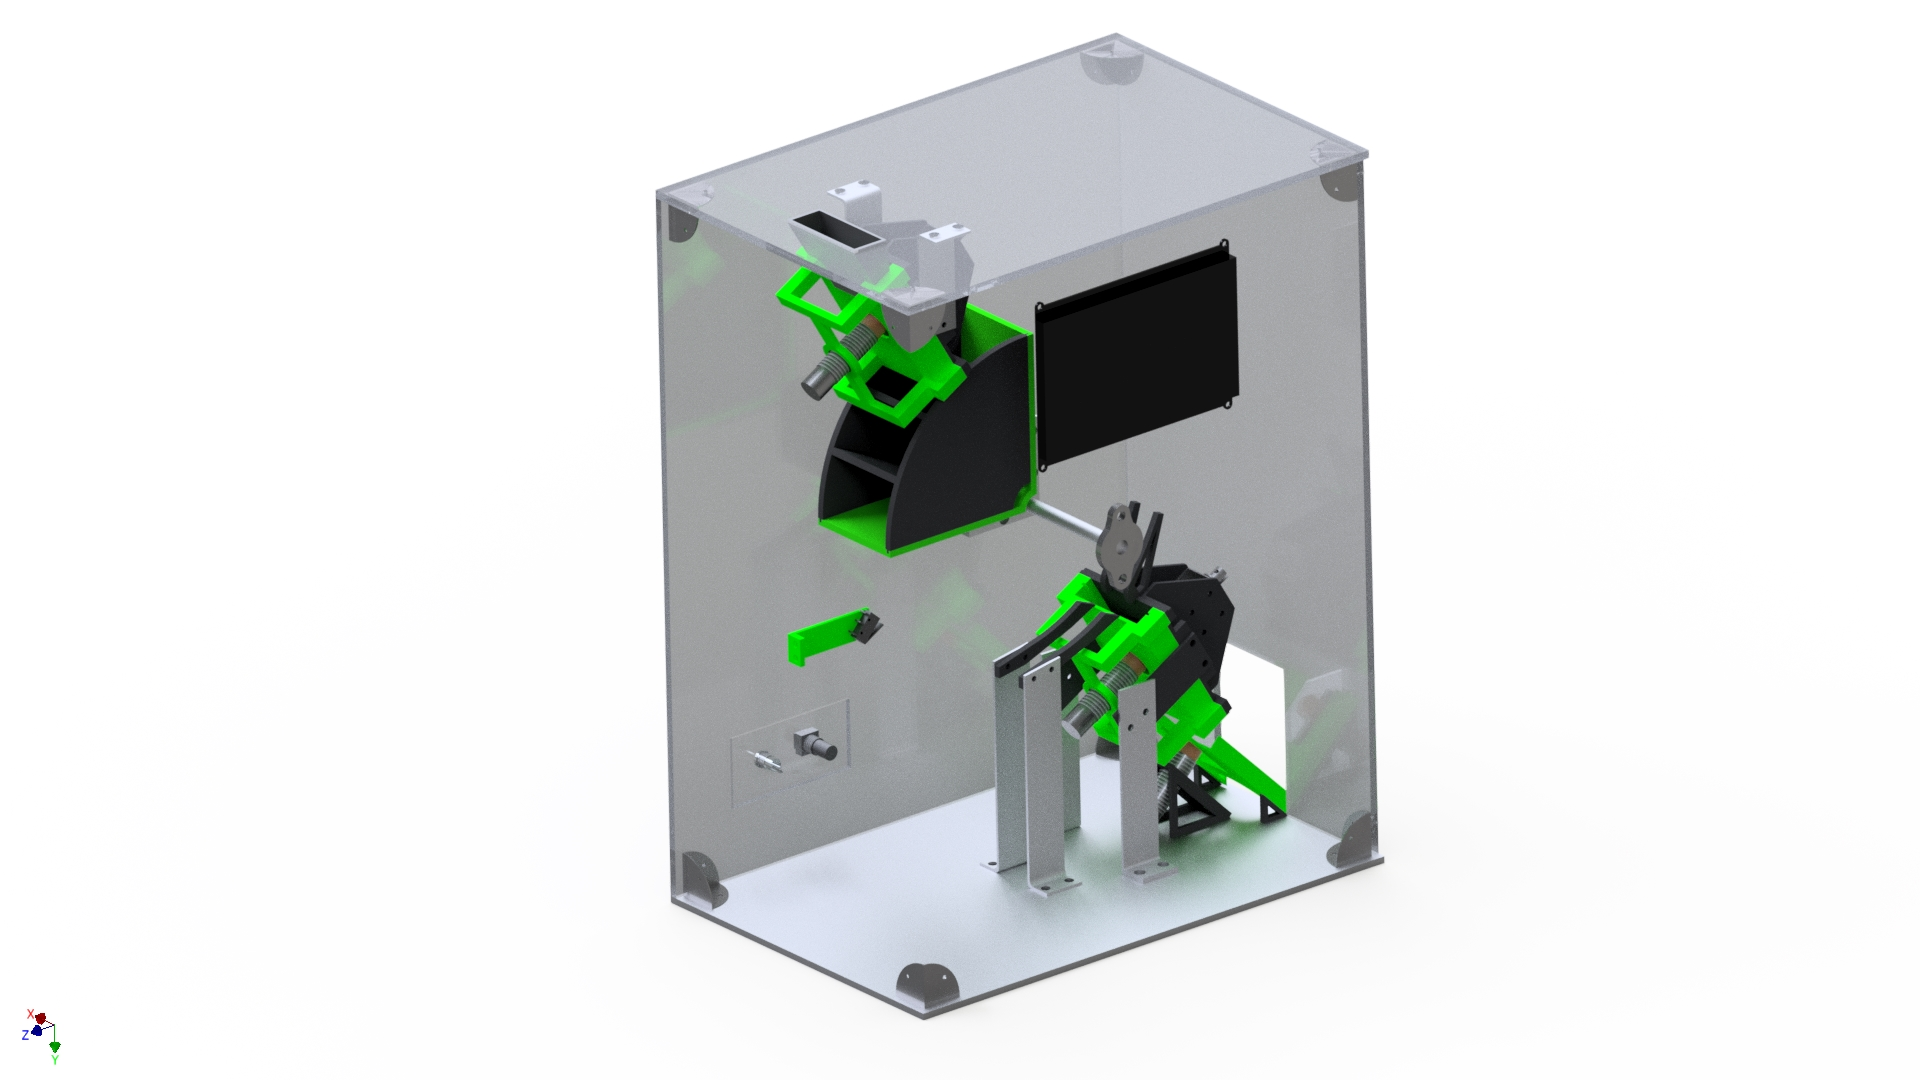
\includegraphics[scale=0.7,page=1]{fig/mech/ReShuffledCombined}
    \caption{Gerendertes Gesamtsystem}
    \label{fig:Gesamtsystem}
\end{figure}

Im \autoref{fig:Gesamtsystem} wird ein Rendering des Gesamtsystems gezeigt.
Bei dem Rendering wurden die beiden vorderen Polycarbonatplatte entfernt, um eine bessere Einsicht in das Gesamtsystem zu erlangen.
Das Rendering besitzt die gleichen Farbtöne wie das gebaute Gesamtsystem sowie die gleichen Dimensionen.

\subsection{Aufgetretene Probleme, Lösungsansätzte und Lösungen}
Beim Teilaufbau des Automaten sind verschiedene Probleme aufgetreten, diese werden in diesen Unterkapiteln bearbeitet und beschrieben.

\subsubsection{Verschließen des Gehäuses}
Da wir unser Gehäuse mit jeweils drei Schrauben und drei Muttern über acht Winkel verschrauben, benötigen
wir eine Lösung, um die letzte Platte des Gehäuses anzuschrauben, da bei dieser die Muttern auf der Unterseite nicht mehr erreichbar sind.
Der billigste und schnellste Lösungsweg wäre,
die jeweilige Muttern an den vier Winkel der TopPlatte zu verschweißen oder zu kleben, sodass sie genau über der
Bohrung sitzen und zum Anschrauben nicht mehr erreichbar sein müssen.

\subsubsection{Durchhängen des Lagerradmoduls}
Weil sich bei dem Lagerradmodul eine Kupplung befindet, kam es dazu, dass ein leichter Knick
auf der Höhe der Kupplung entstand.
Dies führte zwar zu keinem Problem, da der Abstand zwischen den Baugruppen groß genug dimensioniert ist, um gewisse Abweichungen der Bauteile und somit im
vorgegeben Bewegungsablauf auszugleichen.
Falls dies aber dennoch ein Problem darstellen würde, könnte eine andere Kupplung ausgewählt werden, die aktuelle benutzte Kupplung versteift werden oder
man könnte die beiden Wellen des Lagerradmoduls so befestigen, dass sie unter
Zugspannung stehen und somit das Knicken der Kupplung minimieren.

\subsubsection{Verschrauben des Displays}
Da das Display über vier Bohrungen mit der Seitenplatte-Motor verschraubt wird, mussten diese
beim Bearbeiten des Polycarbonats eingezeichnet und gebohrt werden.
Jedoch wurden die Maße des Displays falsch vermessen, und somit stimmten die Bohrungen und der Ausschnitt
der Fräsung nicht mit dem Display überein.
Um dieses Problem zu lösen, und die Vorderseite des Gehäuses dennoch optisch ansprechend zu gestalten, wurden die Bohrungen
des Gehäuses auf Langlochbohrungen erweitert.
Dies löst einerseits das Problem, andererseits
bleibt das Gehäuse durch die bleibende Symmetrie dennoch optisch ansprechend.

\begin{figure}[H]
    \centering
    \includegraphics[scale=0.1,page=1]{fig/mech/DSC00661-removebg.png}
    \caption{Gesamtsystem}
    \label{fig:GesamtsystemEcht}
\end{figure}

In \autoref{fig:GesamtsystemEcht} ist das aufgebaute Gesamtsystem zu sehen.
Bei der Grafik wurden die Kartenentnahme noch nicht an der Maschine befestigt.
Außerdem befinden sich noch keine Platinen in der Maschine.
Um die Maschine optisch ansprechender zu machen, werden die Kabel noch über Kabelführungen in der Maschine verlegt.

\section{Selbstkritische Analyse, Resümee und Ausblick}
\subsection{Verbesserungen}

\subsubsection{Vorausschauend konstruieren}
Viele Konstruktionen wurden schnell gezeichnet und nicht sehr lange durchdacht, daher mussten die Prototypen mehrmals überarbeitet werden.
Dies hätte sich durch genaueres Durchdenken der Konstruktion verhindern lassen können.
Zusätzlich hätte auch die Positionierung einiger Bauteile anders gestaltet werden können, sodass zum Beispiel Schrauben leichter zugänglich sind.

\subsubsection{Fertigungsmethoden}
Anfangs bestanden mehrere Teile noch aus Aluminium und wurden gefräst, jedoch wurden sie später durch 3D-gedruckte
Bauteile ersetzt.
Wäre dies von Anfang an klar gewesen, hätten wir uns Zeit beim Fertigen der Aluminiumteile eingespart.
\subsubsection{Ansaugen der Karten}
Beim Ansaugen der Karten gab es diverse Probleme, da die erste Version nicht mit einem Vakuumsauger funktionierte, sondern
mit einem Sauger, der seinen Unterdruck durch Anpressen erzeugt.
Dieser konnte den erforderlichen Anpressdruck über den Hubmagneten nicht erreichen.
Das Problem löste sich später jedoch mit dem Wechsel zu einem Vakuumsauger.

\subsection{Resümee}
Abschließend ist zu sagen, dass trotz allen erfüllten Bedingungen die Arbeit etwas besser gestaltet hätte werden können.
Aus technischer Sicht hätte mehr Wert auf die Funktion und auf die Stabilität der Bauteile gelegt werden müssen, anstatt
auf die Optik.
Diverse Bauteile hätten einfacher konstruiert werden können, um somit Material und Zeit einzusparen.
Die Kommunikation mit dem Team bereitete keine Komplikationen, jedoch wurde die Zeit, die für das Konstruieren benötigt wurde, unterschätzt.
Auch die Zeit, die für das Produzieren der Teile benötigt wurde, wurde nicht richtig einberechnet, somit
konnten wir uns nicht genau an den geplanten Terminplan halten.
Dennoch wurde die Maschine fertig gebaut, zusammengesetzt
und auf ihre Funktionstüchtigkeit geprüft.

\subsection{Ausblick}
Der funktionierende Automat könnte in Zukunft die Vielfältigkeit der Abteilung Mechatronik und der HTBLA Kaindorf auf
Messen und Veranstaltungen, wie den Tag der offenen Tür, widerspiegeln.